\documentclass[twoside]{book}

% Packages required by doxygen
\usepackage{fixltx2e}
\usepackage{calc}
\usepackage{doxygen}
\usepackage[export]{adjustbox} % also loads graphicx
\usepackage{graphicx}
\usepackage[utf8]{inputenc}
\usepackage{makeidx}
\usepackage{multicol}
\usepackage{multirow}
\PassOptionsToPackage{warn}{textcomp}
\usepackage{textcomp}
\usepackage[nointegrals]{wasysym}
\usepackage[table]{xcolor}

% Font selection
\usepackage[T1]{fontenc}
\usepackage[scaled=.90]{helvet}
\usepackage{courier}
\usepackage{amssymb}
\usepackage{sectsty}
\renewcommand{\familydefault}{\sfdefault}
\allsectionsfont{%
  \fontseries{bc}\selectfont%
  \color{darkgray}%
}
\renewcommand{\DoxyLabelFont}{%
  \fontseries{bc}\selectfont%
  \color{darkgray}%
}
\newcommand{\+}{\discretionary{\mbox{\scriptsize$\hookleftarrow$}}{}{}}

% Page & text layout
\usepackage{geometry}
\geometry{%
  a4paper,%
  top=2.5cm,%
  bottom=2.5cm,%
  left=2.5cm,%
  right=2.5cm%
}
\tolerance=750
\hfuzz=15pt
\hbadness=750
\setlength{\emergencystretch}{15pt}
\setlength{\parindent}{0cm}
\setlength{\parskip}{3ex plus 2ex minus 2ex}
\makeatletter
\renewcommand{\paragraph}{%
  \@startsection{paragraph}{4}{0ex}{-1.0ex}{1.0ex}{%
    \normalfont\normalsize\bfseries\SS@parafont%
  }%
}
\renewcommand{\subparagraph}{%
  \@startsection{subparagraph}{5}{0ex}{-1.0ex}{1.0ex}{%
    \normalfont\normalsize\bfseries\SS@subparafont%
  }%
}
\makeatother

% Headers & footers
\usepackage{fancyhdr}
\pagestyle{fancyplain}
\fancyhead[LE]{\fancyplain{}{\bfseries\thepage}}
\fancyhead[CE]{\fancyplain{}{}}
\fancyhead[RE]{\fancyplain{}{\bfseries\leftmark}}
\fancyhead[LO]{\fancyplain{}{\bfseries\rightmark}}
\fancyhead[CO]{\fancyplain{}{}}
\fancyhead[RO]{\fancyplain{}{\bfseries\thepage}}
\fancyfoot[LE]{\fancyplain{}{}}
\fancyfoot[CE]{\fancyplain{}{}}
\fancyfoot[RE]{\fancyplain{}{\bfseries\scriptsize Generated by Doxygen }}
\fancyfoot[LO]{\fancyplain{}{\bfseries\scriptsize Generated by Doxygen }}
\fancyfoot[CO]{\fancyplain{}{}}
\fancyfoot[RO]{\fancyplain{}{}}
\renewcommand{\footrulewidth}{0.4pt}
\renewcommand{\chaptermark}[1]{%
  \markboth{#1}{}%
}
\renewcommand{\sectionmark}[1]{%
  \markright{\thesection\ #1}%
}

% Indices & bibliography
\usepackage{natbib}
\usepackage[titles]{tocloft}
\setcounter{tocdepth}{3}
\setcounter{secnumdepth}{5}
\makeindex

% Hyperlinks (required, but should be loaded last)
\usepackage{ifpdf}
\ifpdf
  \usepackage[pdftex,pagebackref=true]{hyperref}
\else
  \usepackage[ps2pdf,pagebackref=true]{hyperref}
\fi
\hypersetup{%
  colorlinks=true,%
  linkcolor=blue,%
  citecolor=blue,%
  unicode%
}

% Custom commands
\newcommand{\clearemptydoublepage}{%
  \newpage{\pagestyle{empty}\cleardoublepage}%
}

\usepackage{caption}
\captionsetup{labelsep=space,justification=centering,font={bf},singlelinecheck=off,skip=4pt,position=top}

%===== C O N T E N T S =====

\begin{document}

% Titlepage & ToC
\hypersetup{pageanchor=false,
             bookmarksnumbered=true,
             pdfencoding=unicode
            }
\pagenumbering{alph}
\begin{titlepage}
\vspace*{7cm}
\begin{center}%
{\Large Fault\+In\+Our\+Pong \\[1ex]\large 1 }\\
\vspace*{1cm}
{\large Generated by Doxygen 1.8.12}\\
\end{center}
\end{titlepage}
\clearemptydoublepage
\pagenumbering{roman}
\tableofcontents
\clearemptydoublepage
\pagenumbering{arabic}
\hypersetup{pageanchor=true}

%--- Begin generated contents ---
\chapter{The main page for the game Fault\+In\+Our\+Pong.}
\label{index}\hypertarget{index}{}\input{index}
\chapter{Namespace Index}
\section{Packages}
Here are the packages with brief descriptions (if available)\+:\begin{DoxyCompactList}
\item\contentsline{section}{\hyperlink{namespacemodel}{model} }{\pageref{namespacemodel}}{}
\item\contentsline{section}{\hyperlink{namespacestart_game}{start\+Game} }{\pageref{namespacestart_game}}{}
\item\contentsline{section}{\hyperlink{namespaceview}{view} }{\pageref{namespaceview}}{}
\end{DoxyCompactList}

\chapter{Hierarchical Index}
\section{Class Hierarchy}
This inheritance list is sorted roughly, but not completely, alphabetically\+:\begin{DoxyCompactList}
\item \contentsline{section}{model.\+Ball}{\pageref{classmodel_1_1_ball}}{}
\item \contentsline{section}{start\+Game.\+Game\+Controller}{\pageref{classstart_game_1_1_game_controller}}{}
\item \contentsline{section}{model.\+Game\+Model}{\pageref{classmodel_1_1_game_model}}{}
\item \contentsline{section}{view.\+Game\+View}{\pageref{classview_1_1_game_view}}{}
\item \contentsline{section}{view.\+High\+Score}{\pageref{classview_1_1_high_score}}{}
\item \contentsline{section}{model.\+Paddle}{\pageref{classmodel_1_1_paddle}}{}
\item \contentsline{section}{model.\+Player}{\pageref{classmodel_1_1_player}}{}
\item \contentsline{section}{start\+Game.\+Pong\+Game}{\pageref{classstart_game_1_1_pong_game}}{}
\item J\+Frame\begin{DoxyCompactList}
\item \contentsline{section}{view.\+Mode}{\pageref{classview_1_1_mode}}{}
\item \contentsline{section}{view.\+Tutorial}{\pageref{classview_1_1_tutorial}}{}
\item \contentsline{section}{view.\+Welcome}{\pageref{classview_1_1_welcome}}{}
\end{DoxyCompactList}
\item J\+Panel\begin{DoxyCompactList}
\item \contentsline{section}{view.\+Pong\+Game\+Display}{\pageref{classview_1_1_pong_game_display}}{}
\end{DoxyCompactList}
\end{DoxyCompactList}

\chapter{Class Index}
\section{Class List}
Here are the classes, structs, unions and interfaces with brief descriptions\+:\begin{DoxyCompactList}
\item\contentsline{section}{\hyperlink{classmodel_1_1_ball}{model.\+Ball} }{\pageref{classmodel_1_1_ball}}{}
\item\contentsline{section}{\hyperlink{classstart_game_1_1_game_controller}{start\+Game.\+Game\+Controller} }{\pageref{classstart_game_1_1_game_controller}}{}
\item\contentsline{section}{\hyperlink{classmodel_1_1_game_model}{model.\+Game\+Model} }{\pageref{classmodel_1_1_game_model}}{}
\item\contentsline{section}{\hyperlink{classview_1_1_game_view}{view.\+Game\+View} }{\pageref{classview_1_1_game_view}}{}
\item\contentsline{section}{\hyperlink{classview_1_1_high_score}{view.\+High\+Score} }{\pageref{classview_1_1_high_score}}{}
\item\contentsline{section}{\hyperlink{classview_1_1_mode}{view.\+Mode} }{\pageref{classview_1_1_mode}}{}
\item\contentsline{section}{\hyperlink{classmodel_1_1_paddle}{model.\+Paddle} }{\pageref{classmodel_1_1_paddle}}{}
\item\contentsline{section}{\hyperlink{classmodel_1_1_player}{model.\+Player} }{\pageref{classmodel_1_1_player}}{}
\item\contentsline{section}{\hyperlink{classstart_game_1_1_pong_game}{start\+Game.\+Pong\+Game} }{\pageref{classstart_game_1_1_pong_game}}{}
\item\contentsline{section}{\hyperlink{classview_1_1_pong_game_display}{view.\+Pong\+Game\+Display} }{\pageref{classview_1_1_pong_game_display}}{}
\item\contentsline{section}{\hyperlink{classview_1_1_tutorial}{view.\+Tutorial} }{\pageref{classview_1_1_tutorial}}{}
\item\contentsline{section}{\hyperlink{classview_1_1_welcome}{view.\+Welcome} }{\pageref{classview_1_1_welcome}}{}
\end{DoxyCompactList}

\chapter{File Index}
\section{File List}
Here is a list of all files with brief descriptions\+:\begin{DoxyCompactList}
\item\contentsline{section}{src/model/\hyperlink{_ball_8java}{Ball.\+java} \\*This class represents a ball on the pong game }{\pageref{_ball_8java}}{}
\item\contentsline{section}{src/model/\hyperlink{_game_model_8java}{Game\+Model.\+java} \\*This class represents a ball on the pong game }{\pageref{_game_model_8java}}{}
\item\contentsline{section}{src/model/\hyperlink{_paddle_8java}{Paddle.\+java} \\*This class defines a paddle }{\pageref{_paddle_8java}}{}
\item\contentsline{section}{src/model/\hyperlink{_player_8java}{Player.\+java} \\*This class represents a player for the game }{\pageref{_player_8java}}{}
\item\contentsline{section}{src/start\+Game/\hyperlink{_game_controller_8java}{Game\+Controller.\+java} \\*This class is the controller for the game }{\pageref{_game_controller_8java}}{}
\item\contentsline{section}{src/start\+Game/\hyperlink{_pong_game_8java}{Pong\+Game.\+java} \\*This class starts the game }{\pageref{_pong_game_8java}}{}
\item\contentsline{section}{src/view/\hyperlink{_game_view_8java}{Game\+View.\+java} \\*This class is the main view model }{\pageref{_game_view_8java}}{}
\item\contentsline{section}{src/view/\hyperlink{_mode_8java}{Mode.\+java} \\*This class create the game mode window }{\pageref{_mode_8java}}{}
\item\contentsline{section}{src/view/\hyperlink{_pong_game_display_8java}{Pong\+Game\+Display.\+java} \\*This class construct the view of the pong game }{\pageref{_pong_game_display_8java}}{}
\item\contentsline{section}{src/view/\hyperlink{_tutorial_8java}{Tutorial.\+java} \\*This class create the tutorial window }{\pageref{_tutorial_8java}}{}
\item\contentsline{section}{src/view/\hyperlink{_welcome_8java}{Welcome.\+java} \\*This class creates the display for welcome page }{\pageref{_welcome_8java}}{}
\end{DoxyCompactList}

\chapter{Namespace Documentation}
\hypertarget{namespacemodel}{}\section{Package model}
\label{namespacemodel}\index{model@{model}}
\subsection*{Classes}
\begin{DoxyCompactItemize}
\item 
class \hyperlink{classmodel_1_1_ball}{Ball}
\item 
class \hyperlink{classmodel_1_1_game_model}{Game\+Model}
\item 
class \hyperlink{classmodel_1_1_paddle}{Paddle}
\item 
class \hyperlink{classmodel_1_1_player}{Player}
\end{DoxyCompactItemize}

\hypertarget{namespacestart_game}{}\section{Package start\+Game}
\label{namespacestart_game}\index{start\+Game@{start\+Game}}
\subsection*{Classes}
\begin{DoxyCompactItemize}
\item 
class \hyperlink{classstart_game_1_1_game_controller}{Game\+Controller}
\item 
class \hyperlink{classstart_game_1_1_pong_game}{Pong\+Game}
\end{DoxyCompactItemize}

\hypertarget{namespaceview}{}\section{Package view}
\label{namespaceview}\index{view@{view}}
\subsection*{Classes}
\begin{DoxyCompactItemize}
\item 
class \hyperlink{classview_1_1_game_view}{Game\+View}
\item 
class \hyperlink{classview_1_1_high_score}{High\+Score}
\item 
class \hyperlink{classview_1_1_mode}{Mode}
\item 
class \hyperlink{classview_1_1_pong_game_display}{Pong\+Game\+Display}
\item 
class \hyperlink{classview_1_1_tutorial}{Tutorial}
\item 
class \hyperlink{classview_1_1_welcome}{Welcome}
\end{DoxyCompactItemize}

\chapter{Class Documentation}
\hypertarget{classmodel_1_1_ball}{}\section{model.\+Ball Class Reference}
\label{classmodel_1_1_ball}\index{model.\+Ball@{model.\+Ball}}
\subsection*{Public Member Functions}
\begin{DoxyCompactItemize}
\item 
\hyperlink{classmodel_1_1_ball_a525ba73a7ce62c810a501d6194402cfc}{Ball} ()
\begin{DoxyCompactList}\small\item\em Constructor for \hyperlink{classmodel_1_1_ball}{Ball}. \end{DoxyCompactList}\item 
void \hyperlink{classmodel_1_1_ball_a14854352d44495abed0928ba16a0ac39}{set\+PositionX} (int x)  throws Arithmetic\+Exception 
\begin{DoxyCompactList}\small\item\em sets the x position of the ball \end{DoxyCompactList}\item 
void \hyperlink{classmodel_1_1_ball_a8902ffdc71a7845ec246fedf586649c7}{set\+PositionY} (int y)  throws Arithmetic\+Exception 
\begin{DoxyCompactList}\small\item\em sets the y position of the ball \end{DoxyCompactList}\item 
int \hyperlink{classmodel_1_1_ball_ad6a8f2229d4bdb3dd755443000eeacdf}{get\+PositionX} ()
\begin{DoxyCompactList}\small\item\em gets the x-\/position of the ball \end{DoxyCompactList}\item 
int \hyperlink{classmodel_1_1_ball_ae5509de430dc00bc02259294aa05c10d}{get\+PositionY} ()
\begin{DoxyCompactList}\small\item\em gets the y-\/position of the ball \end{DoxyCompactList}\item 
int \hyperlink{classmodel_1_1_ball_a46ca8051579a49ae750f965621534d5c}{get\+Size} ()
\begin{DoxyCompactList}\small\item\em gets the size of the ball \end{DoxyCompactList}\end{DoxyCompactItemize}
\subsection*{Private Attributes}
\begin{DoxyCompactItemize}
\item 
int \hyperlink{classmodel_1_1_ball_a706c12dfbaabd03b8423ff2bdde0f5c9}{positionX}
\item 
int \hyperlink{classmodel_1_1_ball_aac5d95f10dd849f8cea43c34300d9649}{positionY}
\item 
final int \hyperlink{classmodel_1_1_ball_ad9a73bce4f016c2bd11fb037bac835c7}{S\+I\+ZE} = 20
\end{DoxyCompactItemize}


\subsection{Constructor \& Destructor Documentation}
\hypertarget{classmodel_1_1_ball_a525ba73a7ce62c810a501d6194402cfc}{}\label{classmodel_1_1_ball_a525ba73a7ce62c810a501d6194402cfc} 
\index{model\+::\+Ball@{model\+::\+Ball}!Ball@{Ball}}
\index{Ball@{Ball}!model\+::\+Ball@{model\+::\+Ball}}
\subsubsection{\texorpdfstring{Ball()}{Ball()}}
{\footnotesize\ttfamily model.\+Ball.\+Ball (\begin{DoxyParamCaption}{ }\end{DoxyParamCaption})}



Constructor for \hyperlink{classmodel_1_1_ball}{Ball}. 

Constructor accepts the x and y position of the ball 

\subsection{Member Function Documentation}
\hypertarget{classmodel_1_1_ball_ad6a8f2229d4bdb3dd755443000eeacdf}{}\label{classmodel_1_1_ball_ad6a8f2229d4bdb3dd755443000eeacdf} 
\index{model\+::\+Ball@{model\+::\+Ball}!get\+PositionX@{get\+PositionX}}
\index{get\+PositionX@{get\+PositionX}!model\+::\+Ball@{model\+::\+Ball}}
\subsubsection{\texorpdfstring{get\+Position\+X()}{getPositionX()}}
{\footnotesize\ttfamily int model.\+Ball.\+get\+PositionX (\begin{DoxyParamCaption}{ }\end{DoxyParamCaption})}



gets the x-\/position of the ball 

\begin{DoxyReturn}{Returns}
positionX 
\end{DoxyReturn}
\hypertarget{classmodel_1_1_ball_ae5509de430dc00bc02259294aa05c10d}{}\label{classmodel_1_1_ball_ae5509de430dc00bc02259294aa05c10d} 
\index{model\+::\+Ball@{model\+::\+Ball}!get\+PositionY@{get\+PositionY}}
\index{get\+PositionY@{get\+PositionY}!model\+::\+Ball@{model\+::\+Ball}}
\subsubsection{\texorpdfstring{get\+Position\+Y()}{getPositionY()}}
{\footnotesize\ttfamily int model.\+Ball.\+get\+PositionY (\begin{DoxyParamCaption}{ }\end{DoxyParamCaption})}



gets the y-\/position of the ball 

\begin{DoxyReturn}{Returns}
positionY 
\end{DoxyReturn}
\hypertarget{classmodel_1_1_ball_a46ca8051579a49ae750f965621534d5c}{}\label{classmodel_1_1_ball_a46ca8051579a49ae750f965621534d5c} 
\index{model\+::\+Ball@{model\+::\+Ball}!get\+Size@{get\+Size}}
\index{get\+Size@{get\+Size}!model\+::\+Ball@{model\+::\+Ball}}
\subsubsection{\texorpdfstring{get\+Size()}{getSize()}}
{\footnotesize\ttfamily int model.\+Ball.\+get\+Size (\begin{DoxyParamCaption}{ }\end{DoxyParamCaption})}



gets the size of the ball 

\begin{DoxyReturn}{Returns}
S\+I\+ZE 
\end{DoxyReturn}
\hypertarget{classmodel_1_1_ball_a14854352d44495abed0928ba16a0ac39}{}\label{classmodel_1_1_ball_a14854352d44495abed0928ba16a0ac39} 
\index{model\+::\+Ball@{model\+::\+Ball}!set\+PositionX@{set\+PositionX}}
\index{set\+PositionX@{set\+PositionX}!model\+::\+Ball@{model\+::\+Ball}}
\subsubsection{\texorpdfstring{set\+Position\+X()}{setPositionX()}}
{\footnotesize\ttfamily void model.\+Ball.\+set\+PositionX (\begin{DoxyParamCaption}\item[{int}]{x }\end{DoxyParamCaption}) throws Arithmetic\+Exception}



sets the x position of the ball 


\begin{DoxyParams}{Parameters}
{\em x-\/position} & of the ball \\
\hline
\end{DoxyParams}

\begin{DoxyExceptions}{Exceptions}
{\em Arithmetic\+Exception} & ball x-\/position could not be set out of the game frame. \\
\hline
\end{DoxyExceptions}
\hypertarget{classmodel_1_1_ball_a8902ffdc71a7845ec246fedf586649c7}{}\label{classmodel_1_1_ball_a8902ffdc71a7845ec246fedf586649c7} 
\index{model\+::\+Ball@{model\+::\+Ball}!set\+PositionY@{set\+PositionY}}
\index{set\+PositionY@{set\+PositionY}!model\+::\+Ball@{model\+::\+Ball}}
\subsubsection{\texorpdfstring{set\+Position\+Y()}{setPositionY()}}
{\footnotesize\ttfamily void model.\+Ball.\+set\+PositionY (\begin{DoxyParamCaption}\item[{int}]{y }\end{DoxyParamCaption}) throws Arithmetic\+Exception}



sets the y position of the ball 


\begin{DoxyParams}{Parameters}
{\em y-\/position} & of the ball \\
\hline
\end{DoxyParams}

\begin{DoxyExceptions}{Exceptions}
{\em Arithmetic\+Exception} & ball y-\/position could not be set out of the game frame. \\
\hline
\end{DoxyExceptions}


\subsection{Member Data Documentation}
\hypertarget{classmodel_1_1_ball_a706c12dfbaabd03b8423ff2bdde0f5c9}{}\label{classmodel_1_1_ball_a706c12dfbaabd03b8423ff2bdde0f5c9} 
\index{model\+::\+Ball@{model\+::\+Ball}!positionX@{positionX}}
\index{positionX@{positionX}!model\+::\+Ball@{model\+::\+Ball}}
\subsubsection{\texorpdfstring{positionX}{positionX}}
{\footnotesize\ttfamily int model.\+Ball.\+positionX\hspace{0.3cm}{\ttfamily [private]}}

The X and Y position of a ball on the screen \hypertarget{classmodel_1_1_ball_aac5d95f10dd849f8cea43c34300d9649}{}\label{classmodel_1_1_ball_aac5d95f10dd849f8cea43c34300d9649} 
\index{model\+::\+Ball@{model\+::\+Ball}!positionY@{positionY}}
\index{positionY@{positionY}!model\+::\+Ball@{model\+::\+Ball}}
\subsubsection{\texorpdfstring{positionY}{positionY}}
{\footnotesize\ttfamily int model.\+Ball.\+positionY\hspace{0.3cm}{\ttfamily [private]}}

\hypertarget{classmodel_1_1_ball_ad9a73bce4f016c2bd11fb037bac835c7}{}\label{classmodel_1_1_ball_ad9a73bce4f016c2bd11fb037bac835c7} 
\index{model\+::\+Ball@{model\+::\+Ball}!S\+I\+ZE@{S\+I\+ZE}}
\index{S\+I\+ZE@{S\+I\+ZE}!model\+::\+Ball@{model\+::\+Ball}}
\subsubsection{\texorpdfstring{S\+I\+ZE}{SIZE}}
{\footnotesize\ttfamily final int model.\+Ball.\+S\+I\+ZE = 20\hspace{0.3cm}{\ttfamily [private]}}

The size of a ball 

The documentation for this class was generated from the following file\+:\begin{DoxyCompactItemize}
\item 
src/model/\hyperlink{_ball_8java}{Ball.\+java}\end{DoxyCompactItemize}

\hypertarget{classstart_game_1_1_game_controller}{}\section{start\+Game.\+Game\+Controller Class Reference}
\label{classstart_game_1_1_game_controller}\index{start\+Game.\+Game\+Controller@{start\+Game.\+Game\+Controller}}
\subsection*{Classes}
\begin{DoxyCompactItemize}
\item 
class {\bfseries Game\+Listener}
\begin{DoxyCompactList}\small\item\em action listener for the game page \end{DoxyCompactList}\item 
class {\bfseries Mode\+Listener}
\begin{DoxyCompactList}\small\item\em action listener for the game mode page \end{DoxyCompactList}\item 
class {\bfseries Tutorial\+Listener}
\begin{DoxyCompactList}\small\item\em action listener for the tutorial page \end{DoxyCompactList}\item 
class {\bfseries Welcomepage\+Listener}
\begin{DoxyCompactList}\small\item\em action listener for the welcome page \end{DoxyCompactList}\end{DoxyCompactItemize}
\subsection*{Public Member Functions}
\begin{DoxyCompactItemize}
\item 
\hyperlink{classstart_game_1_1_game_controller_aecc647e49ed23b571160d7d7c68b04d7}{Game\+Controller} (\hyperlink{classview_1_1_game_view}{Game\+View} \hyperlink{classstart_game_1_1_game_controller_a86e3c6ba6e8d0ecb0946da48fa55e7ee}{v}, \hyperlink{classmodel_1_1_game_model}{Game\+Model} \hyperlink{classstart_game_1_1_game_controller_a2c79234f85f979b8f1efe5a48893560d}{m})
\item 
void \hyperlink{classstart_game_1_1_game_controller_abe07c8d60c3adbb0993e637b8c725884}{display} ()
\begin{DoxyCompactList}\small\item\em sets the display \end{DoxyCompactList}\item 
int \hyperlink{classstart_game_1_1_game_controller_a2170345005b5f2f453951dd7b4691e0f}{get\+VelX} ()
\begin{DoxyCompactList}\small\item\em returns the velocity of ball in the x direction. \end{DoxyCompactList}\item 
int \hyperlink{classstart_game_1_1_game_controller_a03bc4dfd9bc501924f18e7f9f49361db}{get\+VelY} ()
\begin{DoxyCompactList}\small\item\em returns the velocity of ball in the y direction. \end{DoxyCompactList}\item 
int \hyperlink{classstart_game_1_1_game_controller_a1b902c1d6b489b6499c340b1db67e868}{getbomb\+VelX} ()
\begin{DoxyCompactList}\small\item\em returns the velocity of bomb in the x direction. \end{DoxyCompactList}\item 
int \hyperlink{classstart_game_1_1_game_controller_a8996d95affa45808c489767da11b6622}{getbomb\+VelY} ()
\begin{DoxyCompactList}\small\item\em returns the velocity of bomb in the y direction. \end{DoxyCompactList}\end{DoxyCompactItemize}
\subsection*{Public Attributes}
\begin{DoxyCompactItemize}
\item 
Hash\+Set$<$ String $>$ \hyperlink{classstart_game_1_1_game_controller_afed267a642ca7f3ec1c1074fec2996dd}{keys} = new Hash\+Set$<$String$>$()
\end{DoxyCompactItemize}
\subsection*{Private Member Functions}
\begin{DoxyCompactItemize}
\item 
void \hyperlink{classstart_game_1_1_game_controller_a3e2fb04603f5a7482672b3b5d1afe568}{check\+Game\+Over} ()
\begin{DoxyCompactList}\small\item\em checks whether the game ends \end{DoxyCompactList}\item 
void \hyperlink{classstart_game_1_1_game_controller_a8b653d5dc322ed45691f1b50dcb16b05}{get\+Elapsed\+Time} ()
\begin{DoxyCompactList}\small\item\em obtains the time the user plays. \end{DoxyCompactList}\item 
void \hyperlink{classstart_game_1_1_game_controller_a2248f03e8a73083a57b10d4faec5797c}{reset\+Game} ()
\begin{DoxyCompactList}\small\item\em resets to initial when the player exits a game. \end{DoxyCompactList}\item 
void \hyperlink{classstart_game_1_1_game_controller_a115fe144ac38f1b8d7e6be4d5bbb23f4}{set\+Speed} ()
\begin{DoxyCompactList}\small\item\em resets speed to ball and bomb \end{DoxyCompactList}\end{DoxyCompactItemize}
\subsection*{Private Attributes}
\begin{DoxyCompactItemize}
\item 
\hyperlink{classview_1_1_game_view}{Game\+View} \hyperlink{classstart_game_1_1_game_controller_a86e3c6ba6e8d0ecb0946da48fa55e7ee}{v}
\item 
\hyperlink{classmodel_1_1_game_model}{Game\+Model} \hyperlink{classstart_game_1_1_game_controller_a2c79234f85f979b8f1efe5a48893560d}{m}
\item 
\hyperlink{classview_1_1_welcome}{Welcome} \hyperlink{classstart_game_1_1_game_controller_a5478c83b51a049015f9d4d6bc5c61607}{w}
\item 
\hyperlink{classview_1_1_mode}{Mode} \hyperlink{classstart_game_1_1_game_controller_ad46f15cbc3846c80495ca340b3b1dedc}{mode}
\item 
\hyperlink{classview_1_1_tutorial}{Tutorial} \hyperlink{classstart_game_1_1_game_controller_ae807267b0bf97687ef3c7d57e815414e}{tut}
\item 
J\+Frame \hyperlink{classstart_game_1_1_game_controller_adc48b19833b682baaa2e189362db5456}{game\+Frame}
\item 
int \hyperlink{classstart_game_1_1_game_controller_a1f16d94b3e5246eb723f9ca04aad4735}{frame\+Width}
\item 
\hyperlink{classview_1_1_pong_game_display}{Pong\+Game\+Display} \hyperlink{classstart_game_1_1_game_controller_aca62497a42166cbb72f5eafbc270afde}{game\+Display}
\item 
int \hyperlink{classstart_game_1_1_game_controller_a9de0dcbec624980f8b3808daa96ef457}{velX} =1
\item 
int \hyperlink{classstart_game_1_1_game_controller_a27e5857e2a63e94e92410f8794064db9}{pad\+Width}
\item 
int \hyperlink{classstart_game_1_1_game_controller_a9969047b4b184c3ea25eeb4ef52dfb1e}{bottom\+PadX}
\item 
\hyperlink{classmodel_1_1_ball}{Ball} \hyperlink{classstart_game_1_1_game_controller_a402855c8c84c77218045cc997a784693}{b}
\item 
\hyperlink{classmodel_1_1_paddle}{Paddle} \hyperlink{classstart_game_1_1_game_controller_a4dc3f50458dc835c6fa67be53fd1751b}{paddle\+\_\+player}
\item 
int \hyperlink{classstart_game_1_1_game_controller_a122256563a1c8df92c4c9d7549f68fd3}{ballX}
\item 
int \hyperlink{classstart_game_1_1_game_controller_af55ee2997cc74f6aee8720fec11f4063}{score\+Top}
\item 
int \hyperlink{classstart_game_1_1_game_controller_a5195c030f589da53f78a185e31a5dc9a}{inset}
\item 
final int \hyperlink{classstart_game_1_1_game_controller_a38526b0e4bd8fd7078ec988678af462d}{S\+I\+N\+G\+LE} = 0
\item 
final int \hyperlink{classstart_game_1_1_game_controller_a36c6fcecafa6f7176733248a5cfb2c87}{A\+D\+V\+A\+N\+CE} = 1
\item 
int \hyperlink{classstart_game_1_1_game_controller_af029ba3e799fe940deb010e575287f55}{game\+Mode}
\item 
\hyperlink{classmodel_1_1_ball}{Ball} \hyperlink{classstart_game_1_1_game_controller_a5196356364a188386c9632e2aed1f105}{bomb}
\item 
int \hyperlink{classstart_game_1_1_game_controller_a9cb60b2c3c52a0c65fcb2480cf52f4e5}{bombX}
\item 
int \hyperlink{classstart_game_1_1_game_controller_a131f6061e92a4e5d4f44d6cfb698dfed}{bomb\+VelX}
\item 
\hyperlink{classmodel_1_1_player}{Player} \hyperlink{classstart_game_1_1_game_controller_ad110380b2d709650ead4b69885fe920e}{player}
\item 
\hyperlink{classmodel_1_1_player}{Player} \hyperlink{classstart_game_1_1_game_controller_a21dfca701ec83511ac399a184530fc63}{ai}
\item 
Timer \hyperlink{classstart_game_1_1_game_controller_af1da0eb8171f6098d28786c5c957fcfd}{t}
\item 
\hyperlink{classview_1_1_high_score}{High\+Score} \hyperlink{classstart_game_1_1_game_controller_a645a34e4b5c875e7fe0dcedc18e8df8a}{display\+Score}
\item 
long \hyperlink{classstart_game_1_1_game_controller_ae22325815bc07ca189abe8e41c94995d}{start\+Time}
\item 
long \hyperlink{classstart_game_1_1_game_controller_a397d65cfee71b4063e05deb55611771f}{end\+Time}
\item 
double \hyperlink{classstart_game_1_1_game_controller_aa63c2f38740966c67d19de8cd4a2a9d0}{time\+Elapsed}
\item 
J\+Button \hyperlink{classstart_game_1_1_game_controller_a4e3d3be632fb6b997c987cb5f516d447}{pause}
\item 
J\+Button \hyperlink{classstart_game_1_1_game_controller_ac9d9ab5f3250992c17d93614754dc0d4}{resume}
\item 
J\+Button \hyperlink{classstart_game_1_1_game_controller_a2a8cdec30f5a04777d2e90d354bb4dd4}{save}
\item 
J\+Button \hyperlink{classstart_game_1_1_game_controller_a188e95237557694a640940111e794c5a}{exit}
\end{DoxyCompactItemize}


\subsection{Constructor \& Destructor Documentation}
\hypertarget{classstart_game_1_1_game_controller_aecc647e49ed23b571160d7d7c68b04d7}{}\label{classstart_game_1_1_game_controller_aecc647e49ed23b571160d7d7c68b04d7} 
\index{start\+Game\+::\+Game\+Controller@{start\+Game\+::\+Game\+Controller}!Game\+Controller@{Game\+Controller}}
\index{Game\+Controller@{Game\+Controller}!start\+Game\+::\+Game\+Controller@{start\+Game\+::\+Game\+Controller}}
\subsubsection{\texorpdfstring{Game\+Controller()}{GameController()}}
{\footnotesize\ttfamily start\+Game.\+Game\+Controller.\+Game\+Controller (\begin{DoxyParamCaption}\item[{\hyperlink{classview_1_1_game_view}{Game\+View}}]{v,  }\item[{\hyperlink{classmodel_1_1_game_model}{Game\+Model}}]{m }\end{DoxyParamCaption})}

Set default game mode to be single

Set up velocities

Obtain the window frame dimentions

Setups for ball in the Model

Setups for the bomb in the Model

Setups for the paddles in the Model
\begin{DoxyItemize}
\item obtain paddle dimensions
\item initialize paddle positions for the player paddle
\item initialize paddle positions for the ai paddle
\end{DoxyItemize}

Setups for the players in the Model
\begin{DoxyItemize}
\item initialize number of life for the player and the ai
\end{DoxyItemize}

Setups for the View
\begin{DoxyItemize}
\item obtain windows from the view
\item add action listener for different windows
\end{DoxyItemize}

Initialize the start time and end time for a player

\subsection{Member Function Documentation}
\hypertarget{classstart_game_1_1_game_controller_a3e2fb04603f5a7482672b3b5d1afe568}{}\label{classstart_game_1_1_game_controller_a3e2fb04603f5a7482672b3b5d1afe568} 
\index{start\+Game\+::\+Game\+Controller@{start\+Game\+::\+Game\+Controller}!check\+Game\+Over@{check\+Game\+Over}}
\index{check\+Game\+Over@{check\+Game\+Over}!start\+Game\+::\+Game\+Controller@{start\+Game\+::\+Game\+Controller}}
\subsubsection{\texorpdfstring{check\+Game\+Over()}{checkGameOver()}}
{\footnotesize\ttfamily void start\+Game.\+Game\+Controller.\+check\+Game\+Over (\begin{DoxyParamCaption}{ }\end{DoxyParamCaption})\hspace{0.3cm}{\ttfamily [private]}}



checks whether the game ends 

check the number of life for both the player and the ai is 0. 
\begin{DoxyItemize}
\item If the number of life for the ai is 0, the player wins
\item If the number of life for the player is 0, the ai wins.
\item Calculate the time a player has played, if breaks the record, save the record.
\end{DoxyItemize}\hypertarget{classstart_game_1_1_game_controller_abe07c8d60c3adbb0993e637b8c725884}{}\label{classstart_game_1_1_game_controller_abe07c8d60c3adbb0993e637b8c725884} 
\index{start\+Game\+::\+Game\+Controller@{start\+Game\+::\+Game\+Controller}!display@{display}}
\index{display@{display}!start\+Game\+::\+Game\+Controller@{start\+Game\+::\+Game\+Controller}}
\subsubsection{\texorpdfstring{display()}{display()}}
{\footnotesize\ttfamily void start\+Game.\+Game\+Controller.\+display (\begin{DoxyParamCaption}{ }\end{DoxyParamCaption})}



sets the display 

opens a window \hypertarget{classstart_game_1_1_game_controller_a1b902c1d6b489b6499c340b1db67e868}{}\label{classstart_game_1_1_game_controller_a1b902c1d6b489b6499c340b1db67e868} 
\index{start\+Game\+::\+Game\+Controller@{start\+Game\+::\+Game\+Controller}!getbomb\+VelX@{getbomb\+VelX}}
\index{getbomb\+VelX@{getbomb\+VelX}!start\+Game\+::\+Game\+Controller@{start\+Game\+::\+Game\+Controller}}
\subsubsection{\texorpdfstring{getbomb\+Vel\+X()}{getbombVelX()}}
{\footnotesize\ttfamily int start\+Game.\+Game\+Controller.\+getbomb\+VelX (\begin{DoxyParamCaption}{ }\end{DoxyParamCaption})}



returns the velocity of bomb in the x direction. 

\begin{DoxyReturn}{Returns}
bomb\+VelX 
\end{DoxyReturn}
\hypertarget{classstart_game_1_1_game_controller_a8996d95affa45808c489767da11b6622}{}\label{classstart_game_1_1_game_controller_a8996d95affa45808c489767da11b6622} 
\index{start\+Game\+::\+Game\+Controller@{start\+Game\+::\+Game\+Controller}!getbomb\+VelY@{getbomb\+VelY}}
\index{getbomb\+VelY@{getbomb\+VelY}!start\+Game\+::\+Game\+Controller@{start\+Game\+::\+Game\+Controller}}
\subsubsection{\texorpdfstring{getbomb\+Vel\+Y()}{getbombVelY()}}
{\footnotesize\ttfamily int start\+Game.\+Game\+Controller.\+getbomb\+VelY (\begin{DoxyParamCaption}{ }\end{DoxyParamCaption})}



returns the velocity of bomb in the y direction. 

\begin{DoxyReturn}{Returns}
bomb\+VelY 
\end{DoxyReturn}
\hypertarget{classstart_game_1_1_game_controller_a8b653d5dc322ed45691f1b50dcb16b05}{}\label{classstart_game_1_1_game_controller_a8b653d5dc322ed45691f1b50dcb16b05} 
\index{start\+Game\+::\+Game\+Controller@{start\+Game\+::\+Game\+Controller}!get\+Elapsed\+Time@{get\+Elapsed\+Time}}
\index{get\+Elapsed\+Time@{get\+Elapsed\+Time}!start\+Game\+::\+Game\+Controller@{start\+Game\+::\+Game\+Controller}}
\subsubsection{\texorpdfstring{get\+Elapsed\+Time()}{getElapsedTime()}}
{\footnotesize\ttfamily void start\+Game.\+Game\+Controller.\+get\+Elapsed\+Time (\begin{DoxyParamCaption}{ }\end{DoxyParamCaption})\hspace{0.3cm}{\ttfamily [private]}}



obtains the time the user plays. 

calculates the time elapsed and save it into a variable. \hypertarget{classstart_game_1_1_game_controller_a2170345005b5f2f453951dd7b4691e0f}{}\label{classstart_game_1_1_game_controller_a2170345005b5f2f453951dd7b4691e0f} 
\index{start\+Game\+::\+Game\+Controller@{start\+Game\+::\+Game\+Controller}!get\+VelX@{get\+VelX}}
\index{get\+VelX@{get\+VelX}!start\+Game\+::\+Game\+Controller@{start\+Game\+::\+Game\+Controller}}
\subsubsection{\texorpdfstring{get\+Vel\+X()}{getVelX()}}
{\footnotesize\ttfamily int start\+Game.\+Game\+Controller.\+get\+VelX (\begin{DoxyParamCaption}{ }\end{DoxyParamCaption})}



returns the velocity of ball in the x direction. 

\begin{DoxyReturn}{Returns}
velX 
\end{DoxyReturn}
\hypertarget{classstart_game_1_1_game_controller_a03bc4dfd9bc501924f18e7f9f49361db}{}\label{classstart_game_1_1_game_controller_a03bc4dfd9bc501924f18e7f9f49361db} 
\index{start\+Game\+::\+Game\+Controller@{start\+Game\+::\+Game\+Controller}!get\+VelY@{get\+VelY}}
\index{get\+VelY@{get\+VelY}!start\+Game\+::\+Game\+Controller@{start\+Game\+::\+Game\+Controller}}
\subsubsection{\texorpdfstring{get\+Vel\+Y()}{getVelY()}}
{\footnotesize\ttfamily int start\+Game.\+Game\+Controller.\+get\+VelY (\begin{DoxyParamCaption}{ }\end{DoxyParamCaption})}



returns the velocity of ball in the y direction. 

\begin{DoxyReturn}{Returns}
velY 
\end{DoxyReturn}
\hypertarget{classstart_game_1_1_game_controller_a2248f03e8a73083a57b10d4faec5797c}{}\label{classstart_game_1_1_game_controller_a2248f03e8a73083a57b10d4faec5797c} 
\index{start\+Game\+::\+Game\+Controller@{start\+Game\+::\+Game\+Controller}!reset\+Game@{reset\+Game}}
\index{reset\+Game@{reset\+Game}!start\+Game\+::\+Game\+Controller@{start\+Game\+::\+Game\+Controller}}
\subsubsection{\texorpdfstring{reset\+Game()}{resetGame()}}
{\footnotesize\ttfamily void start\+Game.\+Game\+Controller.\+reset\+Game (\begin{DoxyParamCaption}{ }\end{DoxyParamCaption})\hspace{0.3cm}{\ttfamily [private]}}



resets to initial when the player exits a game. 

re-\/initializes the variables in the game model and update the variables in view and model. Reset player scores/lives in the model.

Reset the game mode

Reset ball and bomb position

Reset the ball and bomb speed

Re-\/obtain scores/lives from the model

Reset scores in the view\hypertarget{classstart_game_1_1_game_controller_a115fe144ac38f1b8d7e6be4d5bbb23f4}{}\label{classstart_game_1_1_game_controller_a115fe144ac38f1b8d7e6be4d5bbb23f4} 
\index{start\+Game\+::\+Game\+Controller@{start\+Game\+::\+Game\+Controller}!set\+Speed@{set\+Speed}}
\index{set\+Speed@{set\+Speed}!start\+Game\+::\+Game\+Controller@{start\+Game\+::\+Game\+Controller}}
\subsubsection{\texorpdfstring{set\+Speed()}{setSpeed()}}
{\footnotesize\ttfamily void start\+Game.\+Game\+Controller.\+set\+Speed (\begin{DoxyParamCaption}{ }\end{DoxyParamCaption})\hspace{0.3cm}{\ttfamily [private]}}



resets speed to ball and bomb 

re-\/initialize by randomized values Randomize the velocity for bomb

\subsection{Member Data Documentation}
\hypertarget{classstart_game_1_1_game_controller_a36c6fcecafa6f7176733248a5cfb2c87}{}\label{classstart_game_1_1_game_controller_a36c6fcecafa6f7176733248a5cfb2c87} 
\index{start\+Game\+::\+Game\+Controller@{start\+Game\+::\+Game\+Controller}!A\+D\+V\+A\+N\+CE@{A\+D\+V\+A\+N\+CE}}
\index{A\+D\+V\+A\+N\+CE@{A\+D\+V\+A\+N\+CE}!start\+Game\+::\+Game\+Controller@{start\+Game\+::\+Game\+Controller}}
\subsubsection{\texorpdfstring{A\+D\+V\+A\+N\+CE}{ADVANCE}}
{\footnotesize\ttfamily final int start\+Game.\+Game\+Controller.\+A\+D\+V\+A\+N\+CE = 1\hspace{0.3cm}{\ttfamily [private]}}

\hypertarget{classstart_game_1_1_game_controller_a21dfca701ec83511ac399a184530fc63}{}\label{classstart_game_1_1_game_controller_a21dfca701ec83511ac399a184530fc63} 
\index{start\+Game\+::\+Game\+Controller@{start\+Game\+::\+Game\+Controller}!ai@{ai}}
\index{ai@{ai}!start\+Game\+::\+Game\+Controller@{start\+Game\+::\+Game\+Controller}}
\subsubsection{\texorpdfstring{ai}{ai}}
{\footnotesize\ttfamily \hyperlink{classmodel_1_1_player}{Player} start\+Game.\+Game\+Controller.\+ai\hspace{0.3cm}{\ttfamily [private]}}

\hypertarget{classstart_game_1_1_game_controller_a402855c8c84c77218045cc997a784693}{}\label{classstart_game_1_1_game_controller_a402855c8c84c77218045cc997a784693} 
\index{start\+Game\+::\+Game\+Controller@{start\+Game\+::\+Game\+Controller}!b@{b}}
\index{b@{b}!start\+Game\+::\+Game\+Controller@{start\+Game\+::\+Game\+Controller}}
\subsubsection{\texorpdfstring{b}{b}}
{\footnotesize\ttfamily \hyperlink{classmodel_1_1_ball}{Ball} start\+Game.\+Game\+Controller.\+b\hspace{0.3cm}{\ttfamily [private]}}

\hypertarget{classstart_game_1_1_game_controller_a122256563a1c8df92c4c9d7549f68fd3}{}\label{classstart_game_1_1_game_controller_a122256563a1c8df92c4c9d7549f68fd3} 
\index{start\+Game\+::\+Game\+Controller@{start\+Game\+::\+Game\+Controller}!ballX@{ballX}}
\index{ballX@{ballX}!start\+Game\+::\+Game\+Controller@{start\+Game\+::\+Game\+Controller}}
\subsubsection{\texorpdfstring{ballX}{ballX}}
{\footnotesize\ttfamily int start\+Game.\+Game\+Controller.\+ballX\hspace{0.3cm}{\ttfamily [private]}}

\hypertarget{classstart_game_1_1_game_controller_a5196356364a188386c9632e2aed1f105}{}\label{classstart_game_1_1_game_controller_a5196356364a188386c9632e2aed1f105} 
\index{start\+Game\+::\+Game\+Controller@{start\+Game\+::\+Game\+Controller}!bomb@{bomb}}
\index{bomb@{bomb}!start\+Game\+::\+Game\+Controller@{start\+Game\+::\+Game\+Controller}}
\subsubsection{\texorpdfstring{bomb}{bomb}}
{\footnotesize\ttfamily \hyperlink{classmodel_1_1_ball}{Ball} start\+Game.\+Game\+Controller.\+bomb\hspace{0.3cm}{\ttfamily [private]}}

\hypertarget{classstart_game_1_1_game_controller_a131f6061e92a4e5d4f44d6cfb698dfed}{}\label{classstart_game_1_1_game_controller_a131f6061e92a4e5d4f44d6cfb698dfed} 
\index{start\+Game\+::\+Game\+Controller@{start\+Game\+::\+Game\+Controller}!bomb\+VelX@{bomb\+VelX}}
\index{bomb\+VelX@{bomb\+VelX}!start\+Game\+::\+Game\+Controller@{start\+Game\+::\+Game\+Controller}}
\subsubsection{\texorpdfstring{bomb\+VelX}{bombVelX}}
{\footnotesize\ttfamily int start\+Game.\+Game\+Controller.\+bomb\+VelX\hspace{0.3cm}{\ttfamily [private]}}

\hypertarget{classstart_game_1_1_game_controller_a9cb60b2c3c52a0c65fcb2480cf52f4e5}{}\label{classstart_game_1_1_game_controller_a9cb60b2c3c52a0c65fcb2480cf52f4e5} 
\index{start\+Game\+::\+Game\+Controller@{start\+Game\+::\+Game\+Controller}!bombX@{bombX}}
\index{bombX@{bombX}!start\+Game\+::\+Game\+Controller@{start\+Game\+::\+Game\+Controller}}
\subsubsection{\texorpdfstring{bombX}{bombX}}
{\footnotesize\ttfamily int start\+Game.\+Game\+Controller.\+bombX\hspace{0.3cm}{\ttfamily [private]}}

\hypertarget{classstart_game_1_1_game_controller_a9969047b4b184c3ea25eeb4ef52dfb1e}{}\label{classstart_game_1_1_game_controller_a9969047b4b184c3ea25eeb4ef52dfb1e} 
\index{start\+Game\+::\+Game\+Controller@{start\+Game\+::\+Game\+Controller}!bottom\+PadX@{bottom\+PadX}}
\index{bottom\+PadX@{bottom\+PadX}!start\+Game\+::\+Game\+Controller@{start\+Game\+::\+Game\+Controller}}
\subsubsection{\texorpdfstring{bottom\+PadX}{bottomPadX}}
{\footnotesize\ttfamily int start\+Game.\+Game\+Controller.\+bottom\+PadX\hspace{0.3cm}{\ttfamily [private]}}

\hypertarget{classstart_game_1_1_game_controller_a645a34e4b5c875e7fe0dcedc18e8df8a}{}\label{classstart_game_1_1_game_controller_a645a34e4b5c875e7fe0dcedc18e8df8a} 
\index{start\+Game\+::\+Game\+Controller@{start\+Game\+::\+Game\+Controller}!display\+Score@{display\+Score}}
\index{display\+Score@{display\+Score}!start\+Game\+::\+Game\+Controller@{start\+Game\+::\+Game\+Controller}}
\subsubsection{\texorpdfstring{display\+Score}{displayScore}}
{\footnotesize\ttfamily \hyperlink{classview_1_1_high_score}{High\+Score} start\+Game.\+Game\+Controller.\+display\+Score\hspace{0.3cm}{\ttfamily [private]}}

\hypertarget{classstart_game_1_1_game_controller_a397d65cfee71b4063e05deb55611771f}{}\label{classstart_game_1_1_game_controller_a397d65cfee71b4063e05deb55611771f} 
\index{start\+Game\+::\+Game\+Controller@{start\+Game\+::\+Game\+Controller}!end\+Time@{end\+Time}}
\index{end\+Time@{end\+Time}!start\+Game\+::\+Game\+Controller@{start\+Game\+::\+Game\+Controller}}
\subsubsection{\texorpdfstring{end\+Time}{endTime}}
{\footnotesize\ttfamily long start\+Game.\+Game\+Controller.\+end\+Time\hspace{0.3cm}{\ttfamily [private]}}

\hypertarget{classstart_game_1_1_game_controller_a188e95237557694a640940111e794c5a}{}\label{classstart_game_1_1_game_controller_a188e95237557694a640940111e794c5a} 
\index{start\+Game\+::\+Game\+Controller@{start\+Game\+::\+Game\+Controller}!exit@{exit}}
\index{exit@{exit}!start\+Game\+::\+Game\+Controller@{start\+Game\+::\+Game\+Controller}}
\subsubsection{\texorpdfstring{exit}{exit}}
{\footnotesize\ttfamily J\+Button start\+Game.\+Game\+Controller.\+exit\hspace{0.3cm}{\ttfamily [private]}}

\hypertarget{classstart_game_1_1_game_controller_a1f16d94b3e5246eb723f9ca04aad4735}{}\label{classstart_game_1_1_game_controller_a1f16d94b3e5246eb723f9ca04aad4735} 
\index{start\+Game\+::\+Game\+Controller@{start\+Game\+::\+Game\+Controller}!frame\+Width@{frame\+Width}}
\index{frame\+Width@{frame\+Width}!start\+Game\+::\+Game\+Controller@{start\+Game\+::\+Game\+Controller}}
\subsubsection{\texorpdfstring{frame\+Width}{frameWidth}}
{\footnotesize\ttfamily int start\+Game.\+Game\+Controller.\+frame\+Width\hspace{0.3cm}{\ttfamily [private]}}

\hypertarget{classstart_game_1_1_game_controller_aca62497a42166cbb72f5eafbc270afde}{}\label{classstart_game_1_1_game_controller_aca62497a42166cbb72f5eafbc270afde} 
\index{start\+Game\+::\+Game\+Controller@{start\+Game\+::\+Game\+Controller}!game\+Display@{game\+Display}}
\index{game\+Display@{game\+Display}!start\+Game\+::\+Game\+Controller@{start\+Game\+::\+Game\+Controller}}
\subsubsection{\texorpdfstring{game\+Display}{gameDisplay}}
{\footnotesize\ttfamily \hyperlink{classview_1_1_pong_game_display}{Pong\+Game\+Display} start\+Game.\+Game\+Controller.\+game\+Display\hspace{0.3cm}{\ttfamily [private]}}

\hypertarget{classstart_game_1_1_game_controller_adc48b19833b682baaa2e189362db5456}{}\label{classstart_game_1_1_game_controller_adc48b19833b682baaa2e189362db5456} 
\index{start\+Game\+::\+Game\+Controller@{start\+Game\+::\+Game\+Controller}!game\+Frame@{game\+Frame}}
\index{game\+Frame@{game\+Frame}!start\+Game\+::\+Game\+Controller@{start\+Game\+::\+Game\+Controller}}
\subsubsection{\texorpdfstring{game\+Frame}{gameFrame}}
{\footnotesize\ttfamily J\+Frame start\+Game.\+Game\+Controller.\+game\+Frame\hspace{0.3cm}{\ttfamily [private]}}

Variable declarations for the game
\begin{DoxyItemize}
\item frame dimension
\item paddle information
\item ball information
\item bomb information
\item player information 
\end{DoxyItemize}\hypertarget{classstart_game_1_1_game_controller_af029ba3e799fe940deb010e575287f55}{}\label{classstart_game_1_1_game_controller_af029ba3e799fe940deb010e575287f55} 
\index{start\+Game\+::\+Game\+Controller@{start\+Game\+::\+Game\+Controller}!game\+Mode@{game\+Mode}}
\index{game\+Mode@{game\+Mode}!start\+Game\+::\+Game\+Controller@{start\+Game\+::\+Game\+Controller}}
\subsubsection{\texorpdfstring{game\+Mode}{gameMode}}
{\footnotesize\ttfamily int start\+Game.\+Game\+Controller.\+game\+Mode\hspace{0.3cm}{\ttfamily [private]}}

\hypertarget{classstart_game_1_1_game_controller_a5195c030f589da53f78a185e31a5dc9a}{}\label{classstart_game_1_1_game_controller_a5195c030f589da53f78a185e31a5dc9a} 
\index{start\+Game\+::\+Game\+Controller@{start\+Game\+::\+Game\+Controller}!inset@{inset}}
\index{inset@{inset}!start\+Game\+::\+Game\+Controller@{start\+Game\+::\+Game\+Controller}}
\subsubsection{\texorpdfstring{inset}{inset}}
{\footnotesize\ttfamily int start\+Game.\+Game\+Controller.\+inset\hspace{0.3cm}{\ttfamily [private]}}

\hypertarget{classstart_game_1_1_game_controller_afed267a642ca7f3ec1c1074fec2996dd}{}\label{classstart_game_1_1_game_controller_afed267a642ca7f3ec1c1074fec2996dd} 
\index{start\+Game\+::\+Game\+Controller@{start\+Game\+::\+Game\+Controller}!keys@{keys}}
\index{keys@{keys}!start\+Game\+::\+Game\+Controller@{start\+Game\+::\+Game\+Controller}}
\subsubsection{\texorpdfstring{keys}{keys}}
{\footnotesize\ttfamily Hash\+Set$<$String$>$ start\+Game.\+Game\+Controller.\+keys = new Hash\+Set$<$String$>$()}

Declare a variable for storing the key pressed records \hypertarget{classstart_game_1_1_game_controller_a2c79234f85f979b8f1efe5a48893560d}{}\label{classstart_game_1_1_game_controller_a2c79234f85f979b8f1efe5a48893560d} 
\index{start\+Game\+::\+Game\+Controller@{start\+Game\+::\+Game\+Controller}!m@{m}}
\index{m@{m}!start\+Game\+::\+Game\+Controller@{start\+Game\+::\+Game\+Controller}}
\subsubsection{\texorpdfstring{m}{m}}
{\footnotesize\ttfamily \hyperlink{classmodel_1_1_game_model}{Game\+Model} start\+Game.\+Game\+Controller.\+m\hspace{0.3cm}{\ttfamily [private]}}

\hypertarget{classstart_game_1_1_game_controller_ad46f15cbc3846c80495ca340b3b1dedc}{}\label{classstart_game_1_1_game_controller_ad46f15cbc3846c80495ca340b3b1dedc} 
\index{start\+Game\+::\+Game\+Controller@{start\+Game\+::\+Game\+Controller}!mode@{mode}}
\index{mode@{mode}!start\+Game\+::\+Game\+Controller@{start\+Game\+::\+Game\+Controller}}
\subsubsection{\texorpdfstring{mode}{mode}}
{\footnotesize\ttfamily \hyperlink{classview_1_1_mode}{Mode} start\+Game.\+Game\+Controller.\+mode\hspace{0.3cm}{\ttfamily [private]}}

\hypertarget{classstart_game_1_1_game_controller_a4dc3f50458dc835c6fa67be53fd1751b}{}\label{classstart_game_1_1_game_controller_a4dc3f50458dc835c6fa67be53fd1751b} 
\index{start\+Game\+::\+Game\+Controller@{start\+Game\+::\+Game\+Controller}!paddle\+\_\+player@{paddle\+\_\+player}}
\index{paddle\+\_\+player@{paddle\+\_\+player}!start\+Game\+::\+Game\+Controller@{start\+Game\+::\+Game\+Controller}}
\subsubsection{\texorpdfstring{paddle\+\_\+player}{paddle\_player}}
{\footnotesize\ttfamily \hyperlink{classmodel_1_1_paddle}{Paddle} start\+Game.\+Game\+Controller.\+paddle\+\_\+player\hspace{0.3cm}{\ttfamily [private]}}

\hypertarget{classstart_game_1_1_game_controller_a27e5857e2a63e94e92410f8794064db9}{}\label{classstart_game_1_1_game_controller_a27e5857e2a63e94e92410f8794064db9} 
\index{start\+Game\+::\+Game\+Controller@{start\+Game\+::\+Game\+Controller}!pad\+Width@{pad\+Width}}
\index{pad\+Width@{pad\+Width}!start\+Game\+::\+Game\+Controller@{start\+Game\+::\+Game\+Controller}}
\subsubsection{\texorpdfstring{pad\+Width}{padWidth}}
{\footnotesize\ttfamily int start\+Game.\+Game\+Controller.\+pad\+Width\hspace{0.3cm}{\ttfamily [private]}}

\hypertarget{classstart_game_1_1_game_controller_a4e3d3be632fb6b997c987cb5f516d447}{}\label{classstart_game_1_1_game_controller_a4e3d3be632fb6b997c987cb5f516d447} 
\index{start\+Game\+::\+Game\+Controller@{start\+Game\+::\+Game\+Controller}!pause@{pause}}
\index{pause@{pause}!start\+Game\+::\+Game\+Controller@{start\+Game\+::\+Game\+Controller}}
\subsubsection{\texorpdfstring{pause}{pause}}
{\footnotesize\ttfamily J\+Button start\+Game.\+Game\+Controller.\+pause\hspace{0.3cm}{\ttfamily [private]}}

\hypertarget{classstart_game_1_1_game_controller_ad110380b2d709650ead4b69885fe920e}{}\label{classstart_game_1_1_game_controller_ad110380b2d709650ead4b69885fe920e} 
\index{start\+Game\+::\+Game\+Controller@{start\+Game\+::\+Game\+Controller}!player@{player}}
\index{player@{player}!start\+Game\+::\+Game\+Controller@{start\+Game\+::\+Game\+Controller}}
\subsubsection{\texorpdfstring{player}{player}}
{\footnotesize\ttfamily \hyperlink{classmodel_1_1_player}{Player} start\+Game.\+Game\+Controller.\+player\hspace{0.3cm}{\ttfamily [private]}}

\hypertarget{classstart_game_1_1_game_controller_ac9d9ab5f3250992c17d93614754dc0d4}{}\label{classstart_game_1_1_game_controller_ac9d9ab5f3250992c17d93614754dc0d4} 
\index{start\+Game\+::\+Game\+Controller@{start\+Game\+::\+Game\+Controller}!resume@{resume}}
\index{resume@{resume}!start\+Game\+::\+Game\+Controller@{start\+Game\+::\+Game\+Controller}}
\subsubsection{\texorpdfstring{resume}{resume}}
{\footnotesize\ttfamily J\+Button start\+Game.\+Game\+Controller.\+resume\hspace{0.3cm}{\ttfamily [private]}}

\hypertarget{classstart_game_1_1_game_controller_a2a8cdec30f5a04777d2e90d354bb4dd4}{}\label{classstart_game_1_1_game_controller_a2a8cdec30f5a04777d2e90d354bb4dd4} 
\index{start\+Game\+::\+Game\+Controller@{start\+Game\+::\+Game\+Controller}!save@{save}}
\index{save@{save}!start\+Game\+::\+Game\+Controller@{start\+Game\+::\+Game\+Controller}}
\subsubsection{\texorpdfstring{save}{save}}
{\footnotesize\ttfamily J\+Button start\+Game.\+Game\+Controller.\+save\hspace{0.3cm}{\ttfamily [private]}}

\hypertarget{classstart_game_1_1_game_controller_af55ee2997cc74f6aee8720fec11f4063}{}\label{classstart_game_1_1_game_controller_af55ee2997cc74f6aee8720fec11f4063} 
\index{start\+Game\+::\+Game\+Controller@{start\+Game\+::\+Game\+Controller}!score\+Top@{score\+Top}}
\index{score\+Top@{score\+Top}!start\+Game\+::\+Game\+Controller@{start\+Game\+::\+Game\+Controller}}
\subsubsection{\texorpdfstring{score\+Top}{scoreTop}}
{\footnotesize\ttfamily int start\+Game.\+Game\+Controller.\+score\+Top\hspace{0.3cm}{\ttfamily [private]}}

\hypertarget{classstart_game_1_1_game_controller_a38526b0e4bd8fd7078ec988678af462d}{}\label{classstart_game_1_1_game_controller_a38526b0e4bd8fd7078ec988678af462d} 
\index{start\+Game\+::\+Game\+Controller@{start\+Game\+::\+Game\+Controller}!S\+I\+N\+G\+LE@{S\+I\+N\+G\+LE}}
\index{S\+I\+N\+G\+LE@{S\+I\+N\+G\+LE}!start\+Game\+::\+Game\+Controller@{start\+Game\+::\+Game\+Controller}}
\subsubsection{\texorpdfstring{S\+I\+N\+G\+LE}{SINGLE}}
{\footnotesize\ttfamily final int start\+Game.\+Game\+Controller.\+S\+I\+N\+G\+LE = 0\hspace{0.3cm}{\ttfamily [private]}}

\hypertarget{classstart_game_1_1_game_controller_ae22325815bc07ca189abe8e41c94995d}{}\label{classstart_game_1_1_game_controller_ae22325815bc07ca189abe8e41c94995d} 
\index{start\+Game\+::\+Game\+Controller@{start\+Game\+::\+Game\+Controller}!start\+Time@{start\+Time}}
\index{start\+Time@{start\+Time}!start\+Game\+::\+Game\+Controller@{start\+Game\+::\+Game\+Controller}}
\subsubsection{\texorpdfstring{start\+Time}{startTime}}
{\footnotesize\ttfamily long start\+Game.\+Game\+Controller.\+start\+Time\hspace{0.3cm}{\ttfamily [private]}}

\hypertarget{classstart_game_1_1_game_controller_af1da0eb8171f6098d28786c5c957fcfd}{}\label{classstart_game_1_1_game_controller_af1da0eb8171f6098d28786c5c957fcfd} 
\index{start\+Game\+::\+Game\+Controller@{start\+Game\+::\+Game\+Controller}!t@{t}}
\index{t@{t}!start\+Game\+::\+Game\+Controller@{start\+Game\+::\+Game\+Controller}}
\subsubsection{\texorpdfstring{t}{t}}
{\footnotesize\ttfamily Timer start\+Game.\+Game\+Controller.\+t\hspace{0.3cm}{\ttfamily [private]}}

\hypertarget{classstart_game_1_1_game_controller_aa63c2f38740966c67d19de8cd4a2a9d0}{}\label{classstart_game_1_1_game_controller_aa63c2f38740966c67d19de8cd4a2a9d0} 
\index{start\+Game\+::\+Game\+Controller@{start\+Game\+::\+Game\+Controller}!time\+Elapsed@{time\+Elapsed}}
\index{time\+Elapsed@{time\+Elapsed}!start\+Game\+::\+Game\+Controller@{start\+Game\+::\+Game\+Controller}}
\subsubsection{\texorpdfstring{time\+Elapsed}{timeElapsed}}
{\footnotesize\ttfamily double start\+Game.\+Game\+Controller.\+time\+Elapsed\hspace{0.3cm}{\ttfamily [private]}}

\hypertarget{classstart_game_1_1_game_controller_ae807267b0bf97687ef3c7d57e815414e}{}\label{classstart_game_1_1_game_controller_ae807267b0bf97687ef3c7d57e815414e} 
\index{start\+Game\+::\+Game\+Controller@{start\+Game\+::\+Game\+Controller}!tut@{tut}}
\index{tut@{tut}!start\+Game\+::\+Game\+Controller@{start\+Game\+::\+Game\+Controller}}
\subsubsection{\texorpdfstring{tut}{tut}}
{\footnotesize\ttfamily \hyperlink{classview_1_1_tutorial}{Tutorial} start\+Game.\+Game\+Controller.\+tut\hspace{0.3cm}{\ttfamily [private]}}

\hypertarget{classstart_game_1_1_game_controller_a86e3c6ba6e8d0ecb0946da48fa55e7ee}{}\label{classstart_game_1_1_game_controller_a86e3c6ba6e8d0ecb0946da48fa55e7ee} 
\index{start\+Game\+::\+Game\+Controller@{start\+Game\+::\+Game\+Controller}!v@{v}}
\index{v@{v}!start\+Game\+::\+Game\+Controller@{start\+Game\+::\+Game\+Controller}}
\subsubsection{\texorpdfstring{v}{v}}
{\footnotesize\ttfamily \hyperlink{classview_1_1_game_view}{Game\+View} start\+Game.\+Game\+Controller.\+v\hspace{0.3cm}{\ttfamily [private]}}

Import model and view to the controller (this interface). \hypertarget{classstart_game_1_1_game_controller_a9de0dcbec624980f8b3808daa96ef457}{}\label{classstart_game_1_1_game_controller_a9de0dcbec624980f8b3808daa96ef457} 
\index{start\+Game\+::\+Game\+Controller@{start\+Game\+::\+Game\+Controller}!velX@{velX}}
\index{velX@{velX}!start\+Game\+::\+Game\+Controller@{start\+Game\+::\+Game\+Controller}}
\subsubsection{\texorpdfstring{velX}{velX}}
{\footnotesize\ttfamily int start\+Game.\+Game\+Controller.\+velX =1\hspace{0.3cm}{\ttfamily [private]}}

\hypertarget{classstart_game_1_1_game_controller_a5478c83b51a049015f9d4d6bc5c61607}{}\label{classstart_game_1_1_game_controller_a5478c83b51a049015f9d4d6bc5c61607} 
\index{start\+Game\+::\+Game\+Controller@{start\+Game\+::\+Game\+Controller}!w@{w}}
\index{w@{w}!start\+Game\+::\+Game\+Controller@{start\+Game\+::\+Game\+Controller}}
\subsubsection{\texorpdfstring{w}{w}}
{\footnotesize\ttfamily \hyperlink{classview_1_1_welcome}{Welcome} start\+Game.\+Game\+Controller.\+w\hspace{0.3cm}{\ttfamily [private]}}

Variable declarations for storing the game view windows
\begin{DoxyItemize}
\item welcome page
\item mode page for showing different modes
\item tutorial page for giving instructions to the students 
\end{DoxyItemize}

The documentation for this class was generated from the following file\+:\begin{DoxyCompactItemize}
\item 
src/start\+Game/\hyperlink{_game_controller_8java}{Game\+Controller.\+java}\end{DoxyCompactItemize}

\hypertarget{classmodel_1_1_game_model}{}\section{model.\+Game\+Model Class Reference}
\label{classmodel_1_1_game_model}\index{model.\+Game\+Model@{model.\+Game\+Model}}
\subsection*{Public Member Functions}
\begin{DoxyCompactItemize}
\item 
\hyperlink{classmodel_1_1_game_model_a9b1b28ce881943f0f4035cf5fbd3860d}{Game\+Model} ()
\begin{DoxyCompactList}\small\item\em Constructor for the game Model. \end{DoxyCompactList}\item 
void \hyperlink{classmodel_1_1_game_model_a76b4c67d259ce96f0bd20f6c27284ac0}{set\+Ball} (int x, int y)
\begin{DoxyCompactList}\small\item\em sets the x and y positions of a ball \end{DoxyCompactList}\item 
void \hyperlink{classmodel_1_1_game_model_af426dea55d8fff1227dea8bb74530611}{set\+Bomb} (int x, int y)
\begin{DoxyCompactList}\small\item\em sets the x and y positions of a bomb \end{DoxyCompactList}\item 
\hyperlink{classmodel_1_1_ball}{Ball} \hyperlink{classmodel_1_1_game_model_a8523896367260852dad583e37651f87c}{get\+Ball} ()
\begin{DoxyCompactList}\small\item\em gets the \hyperlink{classmodel_1_1_ball}{Ball} object \end{DoxyCompactList}\item 
\hyperlink{classmodel_1_1_ball}{Ball} \hyperlink{classmodel_1_1_game_model_aa53f717eeb13366ffe506363efd1637f}{get\+Bomb} ()
\begin{DoxyCompactList}\small\item\em gets the bomb object \end{DoxyCompactList}\item 
\hyperlink{classmodel_1_1_paddle}{Paddle} \hyperlink{classmodel_1_1_game_model_a8bdb8971824c753c8074ccc0fadf56fc}{get\+Player\+Paddle} ()
\begin{DoxyCompactList}\small\item\em gets the user paddle object \end{DoxyCompactList}\item 
\hyperlink{classmodel_1_1_paddle}{Paddle} \hyperlink{classmodel_1_1_game_model_a15542a275095daae439adcb8b5782055}{get\+Computer\+Paddle} ()
\begin{DoxyCompactList}\small\item\em gets the computer paddle object \end{DoxyCompactList}\item 
\hyperlink{classmodel_1_1_player}{Player} \hyperlink{classmodel_1_1_game_model_a67c62132a9e3578c642613d54350ca75}{get\+Player} ()
\begin{DoxyCompactList}\small\item\em gets the player object \end{DoxyCompactList}\item 
\hyperlink{classmodel_1_1_player}{Player} \hyperlink{classmodel_1_1_game_model_a0bcf575adf7119282fe0a45e3f6bb5df}{get\+Computer} ()
\begin{DoxyCompactList}\small\item\em gets the computer object \end{DoxyCompactList}\end{DoxyCompactItemize}
\subsection*{Private Attributes}
\begin{DoxyCompactItemize}
\item 
\hyperlink{classmodel_1_1_ball}{Ball} \hyperlink{classmodel_1_1_game_model_a1b56c649031a3fb9c0b2930edf719de3}{b}
\item 
\hyperlink{classmodel_1_1_paddle}{Paddle} \hyperlink{classmodel_1_1_game_model_a46b846cead279b52545bb014f946fe47}{p\+\_\+player}
\item 
\hyperlink{classmodel_1_1_player}{Player} \hyperlink{classmodel_1_1_game_model_aa7997c685bdb47e1af57ea496f4128c0}{player}
\end{DoxyCompactItemize}


\subsection{Constructor \& Destructor Documentation}
\hypertarget{classmodel_1_1_game_model_a9b1b28ce881943f0f4035cf5fbd3860d}{}\label{classmodel_1_1_game_model_a9b1b28ce881943f0f4035cf5fbd3860d} 
\index{model\+::\+Game\+Model@{model\+::\+Game\+Model}!Game\+Model@{Game\+Model}}
\index{Game\+Model@{Game\+Model}!model\+::\+Game\+Model@{model\+::\+Game\+Model}}
\subsubsection{\texorpdfstring{Game\+Model()}{GameModel()}}
{\footnotesize\ttfamily model.\+Game\+Model.\+Game\+Model (\begin{DoxyParamCaption}{ }\end{DoxyParamCaption})}



Constructor for the game Model. 

Contains all the data and models for the game, including the player, paddle, and the ball. Declara variables/instances for the model
\begin{DoxyItemize}
\item regular ball
\item bomb
\item paddle for the player
\item paddle for the computer
\item score and life for the player
\item score and life for the ai
\end{DoxyItemize}

\subsection{Member Function Documentation}
\hypertarget{classmodel_1_1_game_model_a8523896367260852dad583e37651f87c}{}\label{classmodel_1_1_game_model_a8523896367260852dad583e37651f87c} 
\index{model\+::\+Game\+Model@{model\+::\+Game\+Model}!get\+Ball@{get\+Ball}}
\index{get\+Ball@{get\+Ball}!model\+::\+Game\+Model@{model\+::\+Game\+Model}}
\subsubsection{\texorpdfstring{get\+Ball()}{getBall()}}
{\footnotesize\ttfamily \hyperlink{classmodel_1_1_ball}{Ball} model.\+Game\+Model.\+get\+Ball (\begin{DoxyParamCaption}{ }\end{DoxyParamCaption})}



gets the \hyperlink{classmodel_1_1_ball}{Ball} object 

\begin{DoxyReturn}{Returns}
b is the ball object 
\end{DoxyReturn}
\hypertarget{classmodel_1_1_game_model_aa53f717eeb13366ffe506363efd1637f}{}\label{classmodel_1_1_game_model_aa53f717eeb13366ffe506363efd1637f} 
\index{model\+::\+Game\+Model@{model\+::\+Game\+Model}!get\+Bomb@{get\+Bomb}}
\index{get\+Bomb@{get\+Bomb}!model\+::\+Game\+Model@{model\+::\+Game\+Model}}
\subsubsection{\texorpdfstring{get\+Bomb()}{getBomb()}}
{\footnotesize\ttfamily \hyperlink{classmodel_1_1_ball}{Ball} model.\+Game\+Model.\+get\+Bomb (\begin{DoxyParamCaption}{ }\end{DoxyParamCaption})}



gets the bomb object 

\begin{DoxyReturn}{Returns}
bomb is the bomb object 
\end{DoxyReturn}
\hypertarget{classmodel_1_1_game_model_a0bcf575adf7119282fe0a45e3f6bb5df}{}\label{classmodel_1_1_game_model_a0bcf575adf7119282fe0a45e3f6bb5df} 
\index{model\+::\+Game\+Model@{model\+::\+Game\+Model}!get\+Computer@{get\+Computer}}
\index{get\+Computer@{get\+Computer}!model\+::\+Game\+Model@{model\+::\+Game\+Model}}
\subsubsection{\texorpdfstring{get\+Computer()}{getComputer()}}
{\footnotesize\ttfamily \hyperlink{classmodel_1_1_player}{Player} model.\+Game\+Model.\+get\+Computer (\begin{DoxyParamCaption}{ }\end{DoxyParamCaption})}



gets the computer object 

\begin{DoxyReturn}{Returns}
computer 
\end{DoxyReturn}
\hypertarget{classmodel_1_1_game_model_a15542a275095daae439adcb8b5782055}{}\label{classmodel_1_1_game_model_a15542a275095daae439adcb8b5782055} 
\index{model\+::\+Game\+Model@{model\+::\+Game\+Model}!get\+Computer\+Paddle@{get\+Computer\+Paddle}}
\index{get\+Computer\+Paddle@{get\+Computer\+Paddle}!model\+::\+Game\+Model@{model\+::\+Game\+Model}}
\subsubsection{\texorpdfstring{get\+Computer\+Paddle()}{getComputerPaddle()}}
{\footnotesize\ttfamily \hyperlink{classmodel_1_1_paddle}{Paddle} model.\+Game\+Model.\+get\+Computer\+Paddle (\begin{DoxyParamCaption}{ }\end{DoxyParamCaption})}



gets the computer paddle object 

\begin{DoxyReturn}{Returns}
p\+\_\+computer 
\end{DoxyReturn}
\hypertarget{classmodel_1_1_game_model_a67c62132a9e3578c642613d54350ca75}{}\label{classmodel_1_1_game_model_a67c62132a9e3578c642613d54350ca75} 
\index{model\+::\+Game\+Model@{model\+::\+Game\+Model}!get\+Player@{get\+Player}}
\index{get\+Player@{get\+Player}!model\+::\+Game\+Model@{model\+::\+Game\+Model}}
\subsubsection{\texorpdfstring{get\+Player()}{getPlayer()}}
{\footnotesize\ttfamily \hyperlink{classmodel_1_1_player}{Player} model.\+Game\+Model.\+get\+Player (\begin{DoxyParamCaption}{ }\end{DoxyParamCaption})}



gets the player object 

\begin{DoxyReturn}{Returns}
player 
\end{DoxyReturn}
\hypertarget{classmodel_1_1_game_model_a8bdb8971824c753c8074ccc0fadf56fc}{}\label{classmodel_1_1_game_model_a8bdb8971824c753c8074ccc0fadf56fc} 
\index{model\+::\+Game\+Model@{model\+::\+Game\+Model}!get\+Player\+Paddle@{get\+Player\+Paddle}}
\index{get\+Player\+Paddle@{get\+Player\+Paddle}!model\+::\+Game\+Model@{model\+::\+Game\+Model}}
\subsubsection{\texorpdfstring{get\+Player\+Paddle()}{getPlayerPaddle()}}
{\footnotesize\ttfamily \hyperlink{classmodel_1_1_paddle}{Paddle} model.\+Game\+Model.\+get\+Player\+Paddle (\begin{DoxyParamCaption}{ }\end{DoxyParamCaption})}



gets the user paddle object 

\begin{DoxyReturn}{Returns}
p\+\_\+player 
\end{DoxyReturn}
\hypertarget{classmodel_1_1_game_model_a76b4c67d259ce96f0bd20f6c27284ac0}{}\label{classmodel_1_1_game_model_a76b4c67d259ce96f0bd20f6c27284ac0} 
\index{model\+::\+Game\+Model@{model\+::\+Game\+Model}!set\+Ball@{set\+Ball}}
\index{set\+Ball@{set\+Ball}!model\+::\+Game\+Model@{model\+::\+Game\+Model}}
\subsubsection{\texorpdfstring{set\+Ball()}{setBall()}}
{\footnotesize\ttfamily void model.\+Game\+Model.\+set\+Ball (\begin{DoxyParamCaption}\item[{int}]{x,  }\item[{int}]{y }\end{DoxyParamCaption})}



sets the x and y positions of a ball 


\begin{DoxyParams}{Parameters}
{\em x} & is the x position of the ball \\
\hline
{\em y} & is the y position of the ball \\
\hline
\end{DoxyParams}
\hypertarget{classmodel_1_1_game_model_af426dea55d8fff1227dea8bb74530611}{}\label{classmodel_1_1_game_model_af426dea55d8fff1227dea8bb74530611} 
\index{model\+::\+Game\+Model@{model\+::\+Game\+Model}!set\+Bomb@{set\+Bomb}}
\index{set\+Bomb@{set\+Bomb}!model\+::\+Game\+Model@{model\+::\+Game\+Model}}
\subsubsection{\texorpdfstring{set\+Bomb()}{setBomb()}}
{\footnotesize\ttfamily void model.\+Game\+Model.\+set\+Bomb (\begin{DoxyParamCaption}\item[{int}]{x,  }\item[{int}]{y }\end{DoxyParamCaption})}



sets the x and y positions of a bomb 


\begin{DoxyParams}{Parameters}
{\em x} & is the x position of the bomb \\
\hline
{\em y} & is the y position of the bomb \\
\hline
\end{DoxyParams}


\subsection{Member Data Documentation}
\hypertarget{classmodel_1_1_game_model_a1b56c649031a3fb9c0b2930edf719de3}{}\label{classmodel_1_1_game_model_a1b56c649031a3fb9c0b2930edf719de3} 
\index{model\+::\+Game\+Model@{model\+::\+Game\+Model}!b@{b}}
\index{b@{b}!model\+::\+Game\+Model@{model\+::\+Game\+Model}}
\subsubsection{\texorpdfstring{b}{b}}
{\footnotesize\ttfamily \hyperlink{classmodel_1_1_ball}{Ball} model.\+Game\+Model.\+b\hspace{0.3cm}{\ttfamily [private]}}

The ball object for the game \hypertarget{classmodel_1_1_game_model_a46b846cead279b52545bb014f946fe47}{}\label{classmodel_1_1_game_model_a46b846cead279b52545bb014f946fe47} 
\index{model\+::\+Game\+Model@{model\+::\+Game\+Model}!p\+\_\+player@{p\+\_\+player}}
\index{p\+\_\+player@{p\+\_\+player}!model\+::\+Game\+Model@{model\+::\+Game\+Model}}
\subsubsection{\texorpdfstring{p\+\_\+player}{p\_player}}
{\footnotesize\ttfamily \hyperlink{classmodel_1_1_paddle}{Paddle} model.\+Game\+Model.\+p\+\_\+player\hspace{0.3cm}{\ttfamily [private]}}

The two paddle in the game, one for the player and the other for the computer \hypertarget{classmodel_1_1_game_model_aa7997c685bdb47e1af57ea496f4128c0}{}\label{classmodel_1_1_game_model_aa7997c685bdb47e1af57ea496f4128c0} 
\index{model\+::\+Game\+Model@{model\+::\+Game\+Model}!player@{player}}
\index{player@{player}!model\+::\+Game\+Model@{model\+::\+Game\+Model}}
\subsubsection{\texorpdfstring{player}{player}}
{\footnotesize\ttfamily \hyperlink{classmodel_1_1_player}{Player} model.\+Game\+Model.\+player\hspace{0.3cm}{\ttfamily [private]}}

The two players in the game, one for the user and the other for the computer 

The documentation for this class was generated from the following file\+:\begin{DoxyCompactItemize}
\item 
src/model/\hyperlink{_game_model_8java}{Game\+Model.\+java}\end{DoxyCompactItemize}

\hypertarget{classview_1_1_game_view}{}\section{view.\+Game\+View Class Reference}
\label{classview_1_1_game_view}\index{view.\+Game\+View@{view.\+Game\+View}}
\subsection*{Public Member Functions}
\begin{DoxyCompactItemize}
\item 
\hyperlink{classview_1_1_game_view_a2405d94a94b047f1858e0ac712983b66}{Game\+View} ()
\begin{DoxyCompactList}\small\item\em Constructor for the view. \end{DoxyCompactList}\item 
void \hyperlink{classview_1_1_game_view_a47f32011f21917818ac92ebecba5dc5b}{display} ()
\begin{DoxyCompactList}\small\item\em displays the welcome page. \end{DoxyCompactList}\item 
\hyperlink{classview_1_1_welcome}{Welcome} \hyperlink{classview_1_1_game_view_adaeb63e182332aee35ca0e0591332add}{get\+Welcome} ()
\begin{DoxyCompactList}\small\item\em gets welcome page window \end{DoxyCompactList}\item 
\hyperlink{classview_1_1_mode}{Mode} \hyperlink{classview_1_1_game_view_a427afb80cd453fd611670936793fb556}{getmode} ()
\begin{DoxyCompactList}\small\item\em gets game mode page window \end{DoxyCompactList}\item 
\hyperlink{classview_1_1_pong_game_display}{Pong\+Game\+Display} \hyperlink{classview_1_1_game_view_ae5dd5521b47a1bdc57e2745ff3b11815}{get\+Game} ()
\begin{DoxyCompactList}\small\item\em gets game window \end{DoxyCompactList}\item 
\hyperlink{classview_1_1_tutorial}{Tutorial} \hyperlink{classview_1_1_game_view_af2d07759d1cde26a4a4d8176baeb0739}{get\+Tutorial} ()
\begin{DoxyCompactList}\small\item\em gets tutorial page window \end{DoxyCompactList}\item 
void \hyperlink{classview_1_1_game_view_aabb001fdf15e7c066c9dbc588f720cd6}{create\+Game} ()
\begin{DoxyCompactList}\small\item\em create the game for display \end{DoxyCompactList}\item 
J\+Button \hyperlink{classview_1_1_game_view_aaab8ca9baf7dce65a6a523a4b5c73feb}{get\+Pause} ()
\item 
J\+Button \hyperlink{classview_1_1_game_view_aafa4556cc05c088d2ac204f4b78955ca}{get\+Resume} ()
\item 
J\+Button \hyperlink{classview_1_1_game_view_a0da97c49ae783ad3d07bb71c80d3ed81}{get\+Save} ()
\item 
J\+Button \hyperlink{classview_1_1_game_view_ae143f3589b520f0db09dd77e88a73c06}{get\+Exit} ()
\item 
J\+Panel \hyperlink{classview_1_1_game_view_ab86ae5b0ca06d2ed673f43888d5547e5}{get\+Game\+Option\+Panel} ()
\item 
void \hyperlink{classview_1_1_game_view_aebcb9f8b30adbfe48e8ef77754b74b89}{add\+Button} (J\+Panel panel, J\+Button button, J\+Button prefer)
\item 
J\+Frame \hyperlink{classview_1_1_game_view_a35853d75ec07ee29d9257c1785508f02}{get\+Game\+Frame} ()
\begin{DoxyCompactList}\small\item\em gets game object \end{DoxyCompactList}\item 
void \hyperlink{classview_1_1_game_view_a7320789eb48e8b661a1f3a522ef592fb}{no\+File\+Avail\+Message} ()
\begin{DoxyCompactList}\small\item\em display message for error loading game record \end{DoxyCompactList}\item 
void \hyperlink{classview_1_1_game_view_aba828f9bc44d416b7b7c03f71a927dbb}{cannot\+Load\+Message} ()
\begin{DoxyCompactList}\small\item\em display message for error loading game \end{DoxyCompactList}\item 
void \hyperlink{classview_1_1_game_view_aed2c0f38680b0e4ff2ea31c1618416d9}{game\+Over} (int whichplayer, double time)
\begin{DoxyCompactList}\small\item\em display message for game over \end{DoxyCompactList}\item 
void \hyperlink{classview_1_1_game_view_a67fd4999f1be51ce360b8bba68e87d9c}{tutorial\+Page} (Image\+Icon img)
\begin{DoxyCompactList}\small\item\em create tutorial page \end{DoxyCompactList}\item 
int \hyperlink{classview_1_1_game_view_a729fea181bb79a2767e11f8c7be01711}{get\+Frame\+Width} ()
\begin{DoxyCompactList}\small\item\em gets width of the window \end{DoxyCompactList}\item 
int \hyperlink{classview_1_1_game_view_a741912e646a65f33e3c571002ed0cf22}{get\+Frame\+Height} ()
\begin{DoxyCompactList}\small\item\em gets height of the window \end{DoxyCompactList}\end{DoxyCompactItemize}
\subsection*{Private Attributes}
\begin{DoxyCompactItemize}
\item 
\hyperlink{classview_1_1_welcome}{Welcome} \hyperlink{classview_1_1_game_view_a473510516d38bd1b016321b06962f0b0}{welcome}
\item 
\hyperlink{classview_1_1_mode}{Mode} \hyperlink{classview_1_1_game_view_a805dd6b76de78fe934f8c4287b4988ce}{mode}
\item 
\hyperlink{classview_1_1_pong_game_display}{Pong\+Game\+Display} \hyperlink{classview_1_1_game_view_a40ab8540fabeed491fc81dce3e801370}{ponggame}
\item 
\hyperlink{classview_1_1_tutorial}{Tutorial} \hyperlink{classview_1_1_game_view_a6bc586b3b4e3079253f50adb03864264}{tutorial}
\item 
J\+Frame \hyperlink{classview_1_1_game_view_a7e90e32a71e4cbc5356dd2960290917c}{game\+Frame}
\item 
final int \hyperlink{classview_1_1_game_view_a2ab92f79dc374ff6708c7798697b623a}{F\+R\+A\+M\+E\+W\+I\+D\+TH} = 700
\item 
final int \hyperlink{classview_1_1_game_view_a4883525ad5307e9ac642854eb6db66d1}{F\+R\+A\+M\+E\+H\+E\+I\+G\+HT} = 500
\item 
J\+Button \hyperlink{classview_1_1_game_view_aca05d6a7d46254d509c48b09945b7053}{pause}
\item 
J\+Button \hyperlink{classview_1_1_game_view_a51484e496307a01d4f261b3ab8517171}{resume}
\item 
J\+Button \hyperlink{classview_1_1_game_view_a0c0efd73b4ba0635f2d21d7980407cd0}{save}
\item 
J\+Button \hyperlink{classview_1_1_game_view_a3bf74babf6e5deb5f2c80a8d7b56ad77}{exit}
\item 
J\+Panel \hyperlink{classview_1_1_game_view_aba201c4e7e254be3254ddffba23f563e}{game\+Options}
\end{DoxyCompactItemize}


\subsection{Constructor \& Destructor Documentation}
\hypertarget{classview_1_1_game_view_a2405d94a94b047f1858e0ac712983b66}{}\label{classview_1_1_game_view_a2405d94a94b047f1858e0ac712983b66} 
\index{view\+::\+Game\+View@{view\+::\+Game\+View}!Game\+View@{Game\+View}}
\index{Game\+View@{Game\+View}!view\+::\+Game\+View@{view\+::\+Game\+View}}
\subsubsection{\texorpdfstring{Game\+View()}{GameView()}}
{\footnotesize\ttfamily view.\+Game\+View.\+Game\+View (\begin{DoxyParamCaption}{ }\end{DoxyParamCaption})}



Constructor for the view. 

declares all other windows 
\begin{DoxyItemize}
\item Pass in different windows to this view interface
\item Wait for further invocation
\end{DoxyItemize}

\subsection{Member Function Documentation}
\hypertarget{classview_1_1_game_view_aebcb9f8b30adbfe48e8ef77754b74b89}{}\label{classview_1_1_game_view_aebcb9f8b30adbfe48e8ef77754b74b89} 
\index{view\+::\+Game\+View@{view\+::\+Game\+View}!add\+Button@{add\+Button}}
\index{add\+Button@{add\+Button}!view\+::\+Game\+View@{view\+::\+Game\+View}}
\subsubsection{\texorpdfstring{add\+Button()}{addButton()}}
{\footnotesize\ttfamily void view.\+Game\+View.\+add\+Button (\begin{DoxyParamCaption}\item[{J\+Panel}]{panel,  }\item[{J\+Button}]{button,  }\item[{J\+Button}]{prefer }\end{DoxyParamCaption})}

\hypertarget{classview_1_1_game_view_aba828f9bc44d416b7b7c03f71a927dbb}{}\label{classview_1_1_game_view_aba828f9bc44d416b7b7c03f71a927dbb} 
\index{view\+::\+Game\+View@{view\+::\+Game\+View}!cannot\+Load\+Message@{cannot\+Load\+Message}}
\index{cannot\+Load\+Message@{cannot\+Load\+Message}!view\+::\+Game\+View@{view\+::\+Game\+View}}
\subsubsection{\texorpdfstring{cannot\+Load\+Message()}{cannotLoadMessage()}}
{\footnotesize\ttfamily void view.\+Game\+View.\+cannot\+Load\+Message (\begin{DoxyParamCaption}{ }\end{DoxyParamCaption})}



display message for error loading game 

create a frame for display \hypertarget{classview_1_1_game_view_aabb001fdf15e7c066c9dbc588f720cd6}{}\label{classview_1_1_game_view_aabb001fdf15e7c066c9dbc588f720cd6} 
\index{view\+::\+Game\+View@{view\+::\+Game\+View}!create\+Game@{create\+Game}}
\index{create\+Game@{create\+Game}!view\+::\+Game\+View@{view\+::\+Game\+View}}
\subsubsection{\texorpdfstring{create\+Game()}{createGame()}}
{\footnotesize\ttfamily void view.\+Game\+View.\+create\+Game (\begin{DoxyParamCaption}{ }\end{DoxyParamCaption})}



create the game for display 

create a frame under set dimension for the game \hypertarget{classview_1_1_game_view_a47f32011f21917818ac92ebecba5dc5b}{}\label{classview_1_1_game_view_a47f32011f21917818ac92ebecba5dc5b} 
\index{view\+::\+Game\+View@{view\+::\+Game\+View}!display@{display}}
\index{display@{display}!view\+::\+Game\+View@{view\+::\+Game\+View}}
\subsubsection{\texorpdfstring{display()}{display()}}
{\footnotesize\ttfamily void view.\+Game\+View.\+display (\begin{DoxyParamCaption}{ }\end{DoxyParamCaption})}



displays the welcome page. 

sets the visibility of the window to be true. \hypertarget{classview_1_1_game_view_aed2c0f38680b0e4ff2ea31c1618416d9}{}\label{classview_1_1_game_view_aed2c0f38680b0e4ff2ea31c1618416d9} 
\index{view\+::\+Game\+View@{view\+::\+Game\+View}!game\+Over@{game\+Over}}
\index{game\+Over@{game\+Over}!view\+::\+Game\+View@{view\+::\+Game\+View}}
\subsubsection{\texorpdfstring{game\+Over()}{gameOver()}}
{\footnotesize\ttfamily void view.\+Game\+View.\+game\+Over (\begin{DoxyParamCaption}\item[{int}]{whichplayer,  }\item[{double}]{time }\end{DoxyParamCaption})}



display message for game over 


\begin{DoxyParams}{Parameters}
{\em whichplayer} & is the indicator for the player \\
\hline
\end{DoxyParams}

\begin{DoxyItemize}
\item If the computer wins, display winning message for the computer
\item If the player wins, display winning message for the player
\end{DoxyItemize}\hypertarget{classview_1_1_game_view_ae143f3589b520f0db09dd77e88a73c06}{}\label{classview_1_1_game_view_ae143f3589b520f0db09dd77e88a73c06} 
\index{view\+::\+Game\+View@{view\+::\+Game\+View}!get\+Exit@{get\+Exit}}
\index{get\+Exit@{get\+Exit}!view\+::\+Game\+View@{view\+::\+Game\+View}}
\subsubsection{\texorpdfstring{get\+Exit()}{getExit()}}
{\footnotesize\ttfamily J\+Button view.\+Game\+View.\+get\+Exit (\begin{DoxyParamCaption}{ }\end{DoxyParamCaption})}

\hypertarget{classview_1_1_game_view_a741912e646a65f33e3c571002ed0cf22}{}\label{classview_1_1_game_view_a741912e646a65f33e3c571002ed0cf22} 
\index{view\+::\+Game\+View@{view\+::\+Game\+View}!get\+Frame\+Height@{get\+Frame\+Height}}
\index{get\+Frame\+Height@{get\+Frame\+Height}!view\+::\+Game\+View@{view\+::\+Game\+View}}
\subsubsection{\texorpdfstring{get\+Frame\+Height()}{getFrameHeight()}}
{\footnotesize\ttfamily int view.\+Game\+View.\+get\+Frame\+Height (\begin{DoxyParamCaption}{ }\end{DoxyParamCaption})}



gets height of the window 

\begin{DoxyReturn}{Returns}
F\+R\+A\+M\+E\+H\+E\+I\+G\+HT 
\end{DoxyReturn}
\hypertarget{classview_1_1_game_view_a729fea181bb79a2767e11f8c7be01711}{}\label{classview_1_1_game_view_a729fea181bb79a2767e11f8c7be01711} 
\index{view\+::\+Game\+View@{view\+::\+Game\+View}!get\+Frame\+Width@{get\+Frame\+Width}}
\index{get\+Frame\+Width@{get\+Frame\+Width}!view\+::\+Game\+View@{view\+::\+Game\+View}}
\subsubsection{\texorpdfstring{get\+Frame\+Width()}{getFrameWidth()}}
{\footnotesize\ttfamily int view.\+Game\+View.\+get\+Frame\+Width (\begin{DoxyParamCaption}{ }\end{DoxyParamCaption})}



gets width of the window 

\begin{DoxyReturn}{Returns}
F\+R\+A\+M\+E\+W\+I\+D\+TH 
\end{DoxyReturn}
\hypertarget{classview_1_1_game_view_ae5dd5521b47a1bdc57e2745ff3b11815}{}\label{classview_1_1_game_view_ae5dd5521b47a1bdc57e2745ff3b11815} 
\index{view\+::\+Game\+View@{view\+::\+Game\+View}!get\+Game@{get\+Game}}
\index{get\+Game@{get\+Game}!view\+::\+Game\+View@{view\+::\+Game\+View}}
\subsubsection{\texorpdfstring{get\+Game()}{getGame()}}
{\footnotesize\ttfamily \hyperlink{classview_1_1_pong_game_display}{Pong\+Game\+Display} view.\+Game\+View.\+get\+Game (\begin{DoxyParamCaption}{ }\end{DoxyParamCaption})}



gets game window 

\begin{DoxyReturn}{Returns}
game window object 
\end{DoxyReturn}
\hypertarget{classview_1_1_game_view_a35853d75ec07ee29d9257c1785508f02}{}\label{classview_1_1_game_view_a35853d75ec07ee29d9257c1785508f02} 
\index{view\+::\+Game\+View@{view\+::\+Game\+View}!get\+Game\+Frame@{get\+Game\+Frame}}
\index{get\+Game\+Frame@{get\+Game\+Frame}!view\+::\+Game\+View@{view\+::\+Game\+View}}
\subsubsection{\texorpdfstring{get\+Game\+Frame()}{getGameFrame()}}
{\footnotesize\ttfamily J\+Frame view.\+Game\+View.\+get\+Game\+Frame (\begin{DoxyParamCaption}{ }\end{DoxyParamCaption})}



gets game object 

\begin{DoxyReturn}{Returns}
game object 
\end{DoxyReturn}
\hypertarget{classview_1_1_game_view_ab86ae5b0ca06d2ed673f43888d5547e5}{}\label{classview_1_1_game_view_ab86ae5b0ca06d2ed673f43888d5547e5} 
\index{view\+::\+Game\+View@{view\+::\+Game\+View}!get\+Game\+Option\+Panel@{get\+Game\+Option\+Panel}}
\index{get\+Game\+Option\+Panel@{get\+Game\+Option\+Panel}!view\+::\+Game\+View@{view\+::\+Game\+View}}
\subsubsection{\texorpdfstring{get\+Game\+Option\+Panel()}{getGameOptionPanel()}}
{\footnotesize\ttfamily J\+Panel view.\+Game\+View.\+get\+Game\+Option\+Panel (\begin{DoxyParamCaption}{ }\end{DoxyParamCaption})}

\hypertarget{classview_1_1_game_view_a427afb80cd453fd611670936793fb556}{}\label{classview_1_1_game_view_a427afb80cd453fd611670936793fb556} 
\index{view\+::\+Game\+View@{view\+::\+Game\+View}!getmode@{getmode}}
\index{getmode@{getmode}!view\+::\+Game\+View@{view\+::\+Game\+View}}
\subsubsection{\texorpdfstring{getmode()}{getmode()}}
{\footnotesize\ttfamily \hyperlink{classview_1_1_mode}{Mode} view.\+Game\+View.\+getmode (\begin{DoxyParamCaption}{ }\end{DoxyParamCaption})}



gets game mode page window 

\begin{DoxyReturn}{Returns}
game mode page object 
\end{DoxyReturn}
\hypertarget{classview_1_1_game_view_aaab8ca9baf7dce65a6a523a4b5c73feb}{}\label{classview_1_1_game_view_aaab8ca9baf7dce65a6a523a4b5c73feb} 
\index{view\+::\+Game\+View@{view\+::\+Game\+View}!get\+Pause@{get\+Pause}}
\index{get\+Pause@{get\+Pause}!view\+::\+Game\+View@{view\+::\+Game\+View}}
\subsubsection{\texorpdfstring{get\+Pause()}{getPause()}}
{\footnotesize\ttfamily J\+Button view.\+Game\+View.\+get\+Pause (\begin{DoxyParamCaption}{ }\end{DoxyParamCaption})}

\hypertarget{classview_1_1_game_view_aafa4556cc05c088d2ac204f4b78955ca}{}\label{classview_1_1_game_view_aafa4556cc05c088d2ac204f4b78955ca} 
\index{view\+::\+Game\+View@{view\+::\+Game\+View}!get\+Resume@{get\+Resume}}
\index{get\+Resume@{get\+Resume}!view\+::\+Game\+View@{view\+::\+Game\+View}}
\subsubsection{\texorpdfstring{get\+Resume()}{getResume()}}
{\footnotesize\ttfamily J\+Button view.\+Game\+View.\+get\+Resume (\begin{DoxyParamCaption}{ }\end{DoxyParamCaption})}

\hypertarget{classview_1_1_game_view_a0da97c49ae783ad3d07bb71c80d3ed81}{}\label{classview_1_1_game_view_a0da97c49ae783ad3d07bb71c80d3ed81} 
\index{view\+::\+Game\+View@{view\+::\+Game\+View}!get\+Save@{get\+Save}}
\index{get\+Save@{get\+Save}!view\+::\+Game\+View@{view\+::\+Game\+View}}
\subsubsection{\texorpdfstring{get\+Save()}{getSave()}}
{\footnotesize\ttfamily J\+Button view.\+Game\+View.\+get\+Save (\begin{DoxyParamCaption}{ }\end{DoxyParamCaption})}

\hypertarget{classview_1_1_game_view_af2d07759d1cde26a4a4d8176baeb0739}{}\label{classview_1_1_game_view_af2d07759d1cde26a4a4d8176baeb0739} 
\index{view\+::\+Game\+View@{view\+::\+Game\+View}!get\+Tutorial@{get\+Tutorial}}
\index{get\+Tutorial@{get\+Tutorial}!view\+::\+Game\+View@{view\+::\+Game\+View}}
\subsubsection{\texorpdfstring{get\+Tutorial()}{getTutorial()}}
{\footnotesize\ttfamily \hyperlink{classview_1_1_tutorial}{Tutorial} view.\+Game\+View.\+get\+Tutorial (\begin{DoxyParamCaption}{ }\end{DoxyParamCaption})}



gets tutorial page window 

\begin{DoxyReturn}{Returns}
tutorial page object 
\end{DoxyReturn}
\hypertarget{classview_1_1_game_view_adaeb63e182332aee35ca0e0591332add}{}\label{classview_1_1_game_view_adaeb63e182332aee35ca0e0591332add} 
\index{view\+::\+Game\+View@{view\+::\+Game\+View}!get\+Welcome@{get\+Welcome}}
\index{get\+Welcome@{get\+Welcome}!view\+::\+Game\+View@{view\+::\+Game\+View}}
\subsubsection{\texorpdfstring{get\+Welcome()}{getWelcome()}}
{\footnotesize\ttfamily \hyperlink{classview_1_1_welcome}{Welcome} view.\+Game\+View.\+get\+Welcome (\begin{DoxyParamCaption}{ }\end{DoxyParamCaption})}



gets welcome page window 

\begin{DoxyReturn}{Returns}
welcome page object 
\end{DoxyReturn}
\hypertarget{classview_1_1_game_view_a7320789eb48e8b661a1f3a522ef592fb}{}\label{classview_1_1_game_view_a7320789eb48e8b661a1f3a522ef592fb} 
\index{view\+::\+Game\+View@{view\+::\+Game\+View}!no\+File\+Avail\+Message@{no\+File\+Avail\+Message}}
\index{no\+File\+Avail\+Message@{no\+File\+Avail\+Message}!view\+::\+Game\+View@{view\+::\+Game\+View}}
\subsubsection{\texorpdfstring{no\+File\+Avail\+Message()}{noFileAvailMessage()}}
{\footnotesize\ttfamily void view.\+Game\+View.\+no\+File\+Avail\+Message (\begin{DoxyParamCaption}{ }\end{DoxyParamCaption})}



display message for error loading game record 

create a frame for display \hypertarget{classview_1_1_game_view_a67fd4999f1be51ce360b8bba68e87d9c}{}\label{classview_1_1_game_view_a67fd4999f1be51ce360b8bba68e87d9c} 
\index{view\+::\+Game\+View@{view\+::\+Game\+View}!tutorial\+Page@{tutorial\+Page}}
\index{tutorial\+Page@{tutorial\+Page}!view\+::\+Game\+View@{view\+::\+Game\+View}}
\subsubsection{\texorpdfstring{tutorial\+Page()}{tutorialPage()}}
{\footnotesize\ttfamily void view.\+Game\+View.\+tutorial\+Page (\begin{DoxyParamCaption}\item[{Image\+Icon}]{img }\end{DoxyParamCaption})}



create tutorial page 


\begin{DoxyParams}{Parameters}
{\em img} & is the image for display \\
\hline
\end{DoxyParams}


\subsection{Member Data Documentation}
\hypertarget{classview_1_1_game_view_a3bf74babf6e5deb5f2c80a8d7b56ad77}{}\label{classview_1_1_game_view_a3bf74babf6e5deb5f2c80a8d7b56ad77} 
\index{view\+::\+Game\+View@{view\+::\+Game\+View}!exit@{exit}}
\index{exit@{exit}!view\+::\+Game\+View@{view\+::\+Game\+View}}
\subsubsection{\texorpdfstring{exit}{exit}}
{\footnotesize\ttfamily J\+Button view.\+Game\+View.\+exit\hspace{0.3cm}{\ttfamily [private]}}

\hypertarget{classview_1_1_game_view_a4883525ad5307e9ac642854eb6db66d1}{}\label{classview_1_1_game_view_a4883525ad5307e9ac642854eb6db66d1} 
\index{view\+::\+Game\+View@{view\+::\+Game\+View}!F\+R\+A\+M\+E\+H\+E\+I\+G\+HT@{F\+R\+A\+M\+E\+H\+E\+I\+G\+HT}}
\index{F\+R\+A\+M\+E\+H\+E\+I\+G\+HT@{F\+R\+A\+M\+E\+H\+E\+I\+G\+HT}!view\+::\+Game\+View@{view\+::\+Game\+View}}
\subsubsection{\texorpdfstring{F\+R\+A\+M\+E\+H\+E\+I\+G\+HT}{FRAMEHEIGHT}}
{\footnotesize\ttfamily final int view.\+Game\+View.\+F\+R\+A\+M\+E\+H\+E\+I\+G\+HT = 500\hspace{0.3cm}{\ttfamily [private]}}

\hypertarget{classview_1_1_game_view_a2ab92f79dc374ff6708c7798697b623a}{}\label{classview_1_1_game_view_a2ab92f79dc374ff6708c7798697b623a} 
\index{view\+::\+Game\+View@{view\+::\+Game\+View}!F\+R\+A\+M\+E\+W\+I\+D\+TH@{F\+R\+A\+M\+E\+W\+I\+D\+TH}}
\index{F\+R\+A\+M\+E\+W\+I\+D\+TH@{F\+R\+A\+M\+E\+W\+I\+D\+TH}!view\+::\+Game\+View@{view\+::\+Game\+View}}
\subsubsection{\texorpdfstring{F\+R\+A\+M\+E\+W\+I\+D\+TH}{FRAMEWIDTH}}
{\footnotesize\ttfamily final int view.\+Game\+View.\+F\+R\+A\+M\+E\+W\+I\+D\+TH = 700\hspace{0.3cm}{\ttfamily [private]}}

Constant declarations for the view \hypertarget{classview_1_1_game_view_a7e90e32a71e4cbc5356dd2960290917c}{}\label{classview_1_1_game_view_a7e90e32a71e4cbc5356dd2960290917c} 
\index{view\+::\+Game\+View@{view\+::\+Game\+View}!game\+Frame@{game\+Frame}}
\index{game\+Frame@{game\+Frame}!view\+::\+Game\+View@{view\+::\+Game\+View}}
\subsubsection{\texorpdfstring{game\+Frame}{gameFrame}}
{\footnotesize\ttfamily J\+Frame view.\+Game\+View.\+game\+Frame\hspace{0.3cm}{\ttfamily [private]}}

\hypertarget{classview_1_1_game_view_aba201c4e7e254be3254ddffba23f563e}{}\label{classview_1_1_game_view_aba201c4e7e254be3254ddffba23f563e} 
\index{view\+::\+Game\+View@{view\+::\+Game\+View}!game\+Options@{game\+Options}}
\index{game\+Options@{game\+Options}!view\+::\+Game\+View@{view\+::\+Game\+View}}
\subsubsection{\texorpdfstring{game\+Options}{gameOptions}}
{\footnotesize\ttfamily J\+Panel view.\+Game\+View.\+game\+Options\hspace{0.3cm}{\ttfamily [private]}}

\hypertarget{classview_1_1_game_view_a805dd6b76de78fe934f8c4287b4988ce}{}\label{classview_1_1_game_view_a805dd6b76de78fe934f8c4287b4988ce} 
\index{view\+::\+Game\+View@{view\+::\+Game\+View}!mode@{mode}}
\index{mode@{mode}!view\+::\+Game\+View@{view\+::\+Game\+View}}
\subsubsection{\texorpdfstring{mode}{mode}}
{\footnotesize\ttfamily \hyperlink{classview_1_1_mode}{Mode} view.\+Game\+View.\+mode\hspace{0.3cm}{\ttfamily [private]}}

\hypertarget{classview_1_1_game_view_aca05d6a7d46254d509c48b09945b7053}{}\label{classview_1_1_game_view_aca05d6a7d46254d509c48b09945b7053} 
\index{view\+::\+Game\+View@{view\+::\+Game\+View}!pause@{pause}}
\index{pause@{pause}!view\+::\+Game\+View@{view\+::\+Game\+View}}
\subsubsection{\texorpdfstring{pause}{pause}}
{\footnotesize\ttfamily J\+Button view.\+Game\+View.\+pause\hspace{0.3cm}{\ttfamily [private]}}

Set up buttons on the game panel \hypertarget{classview_1_1_game_view_a40ab8540fabeed491fc81dce3e801370}{}\label{classview_1_1_game_view_a40ab8540fabeed491fc81dce3e801370} 
\index{view\+::\+Game\+View@{view\+::\+Game\+View}!ponggame@{ponggame}}
\index{ponggame@{ponggame}!view\+::\+Game\+View@{view\+::\+Game\+View}}
\subsubsection{\texorpdfstring{ponggame}{ponggame}}
{\footnotesize\ttfamily \hyperlink{classview_1_1_pong_game_display}{Pong\+Game\+Display} view.\+Game\+View.\+ponggame\hspace{0.3cm}{\ttfamily [private]}}

\hypertarget{classview_1_1_game_view_a51484e496307a01d4f261b3ab8517171}{}\label{classview_1_1_game_view_a51484e496307a01d4f261b3ab8517171} 
\index{view\+::\+Game\+View@{view\+::\+Game\+View}!resume@{resume}}
\index{resume@{resume}!view\+::\+Game\+View@{view\+::\+Game\+View}}
\subsubsection{\texorpdfstring{resume}{resume}}
{\footnotesize\ttfamily J\+Button view.\+Game\+View.\+resume\hspace{0.3cm}{\ttfamily [private]}}

\hypertarget{classview_1_1_game_view_a0c0efd73b4ba0635f2d21d7980407cd0}{}\label{classview_1_1_game_view_a0c0efd73b4ba0635f2d21d7980407cd0} 
\index{view\+::\+Game\+View@{view\+::\+Game\+View}!save@{save}}
\index{save@{save}!view\+::\+Game\+View@{view\+::\+Game\+View}}
\subsubsection{\texorpdfstring{save}{save}}
{\footnotesize\ttfamily J\+Button view.\+Game\+View.\+save\hspace{0.3cm}{\ttfamily [private]}}

\hypertarget{classview_1_1_game_view_a6bc586b3b4e3079253f50adb03864264}{}\label{classview_1_1_game_view_a6bc586b3b4e3079253f50adb03864264} 
\index{view\+::\+Game\+View@{view\+::\+Game\+View}!tutorial@{tutorial}}
\index{tutorial@{tutorial}!view\+::\+Game\+View@{view\+::\+Game\+View}}
\subsubsection{\texorpdfstring{tutorial}{tutorial}}
{\footnotesize\ttfamily \hyperlink{classview_1_1_tutorial}{Tutorial} view.\+Game\+View.\+tutorial\hspace{0.3cm}{\ttfamily [private]}}

\hypertarget{classview_1_1_game_view_a473510516d38bd1b016321b06962f0b0}{}\label{classview_1_1_game_view_a473510516d38bd1b016321b06962f0b0} 
\index{view\+::\+Game\+View@{view\+::\+Game\+View}!welcome@{welcome}}
\index{welcome@{welcome}!view\+::\+Game\+View@{view\+::\+Game\+View}}
\subsubsection{\texorpdfstring{welcome}{welcome}}
{\footnotesize\ttfamily \hyperlink{classview_1_1_welcome}{Welcome} view.\+Game\+View.\+welcome\hspace{0.3cm}{\ttfamily [private]}}

Variable declarations to store different pages
\begin{DoxyItemize}
\item welcome page
\item game mode page
\item tutorial page
\item game page 
\end{DoxyItemize}

The documentation for this class was generated from the following file\+:\begin{DoxyCompactItemize}
\item 
src/view/\hyperlink{_game_view_8java}{Game\+View.\+java}\end{DoxyCompactItemize}

\hypertarget{classview_1_1_mode}{}\section{view.\+Mode Class Reference}
\label{classview_1_1_mode}\index{view.\+Mode@{view.\+Mode}}
Inheritance diagram for view.\+Mode\+:\begin{figure}[H]
\begin{center}
\leavevmode
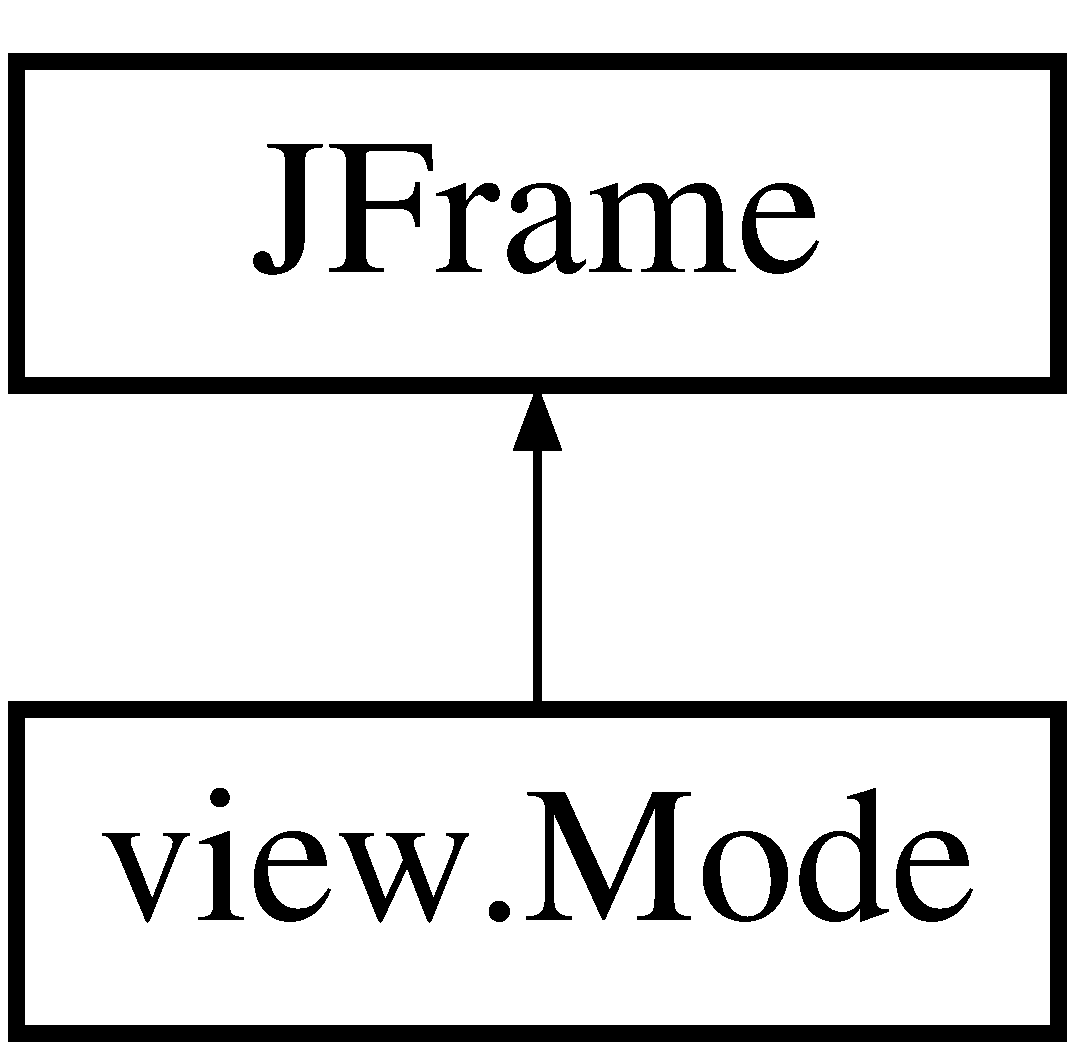
\includegraphics[height=2.000000cm]{classview_1_1_mode}
\end{center}
\end{figure}
\subsection*{Public Member Functions}
\begin{DoxyCompactItemize}
\item 
\hyperlink{classview_1_1_mode_a55b668b8551b43596ab48afb749faec0}{Mode} ()
\begin{DoxyCompactList}\small\item\em Constructor for the player. \end{DoxyCompactList}\item 
void \hyperlink{classview_1_1_mode_a133b1b524c5ac2bb62da0f7f892c006d}{add\+Button} (J\+Button x)
\begin{DoxyCompactList}\small\item\em adds buttons to a panel \end{DoxyCompactList}\item 
void \hyperlink{classview_1_1_mode_a0f731453457f37dd1f3b16994a398c3e}{add\+Listener} (Action\+Listener button\+Listener)
\begin{DoxyCompactList}\small\item\em adds action listener to the buttons \end{DoxyCompactList}\item 
J\+Button \hyperlink{classview_1_1_mode_ad97ed0dc0beeb1f54affe3355846bf6a}{get\+Single} ()
\begin{DoxyCompactList}\small\item\em gets the button for single mode \end{DoxyCompactList}\end{DoxyCompactItemize}
\subsection*{Private Attributes}
\begin{DoxyCompactItemize}
\item 
J\+Button \hyperlink{classview_1_1_mode_a79eea473b39369327297c8788dd071c2}{single} = new J\+Button(\char`\"{}Single \hyperlink{classmodel_1_1_player}{Player} \hyperlink{classview_1_1_mode}{Mode}\char`\"{})
\item 
J\+Button \hyperlink{classview_1_1_mode_a015d017e7fa759ee77d191c4d03ee531}{s\+Obstacle} = new J\+Button(\char`\"{}Advanced Single \hyperlink{classmodel_1_1_player}{Player} \hyperlink{classview_1_1_mode}{Mode}\char`\"{})
\item 
J\+Panel \hyperlink{classview_1_1_mode_ab457e88b13dca6e72659a05f9d6d7853}{button\+Panel}
\end{DoxyCompactItemize}


\subsection{Constructor \& Destructor Documentation}
\hypertarget{classview_1_1_mode_a55b668b8551b43596ab48afb749faec0}{}\label{classview_1_1_mode_a55b668b8551b43596ab48afb749faec0} 
\index{view\+::\+Mode@{view\+::\+Mode}!Mode@{Mode}}
\index{Mode@{Mode}!view\+::\+Mode@{view\+::\+Mode}}
\subsubsection{\texorpdfstring{Mode()}{Mode()}}
{\footnotesize\ttfamily view.\+Mode.\+Mode (\begin{DoxyParamCaption}{ }\end{DoxyParamCaption})}



Constructor for the player. 

sets the size and header for the window, and adds buttons to the window Setups for the frame

Setups for the buttons on the panel

Add the panel to the frame/window for display

\subsection{Member Function Documentation}
\hypertarget{classview_1_1_mode_a133b1b524c5ac2bb62da0f7f892c006d}{}\label{classview_1_1_mode_a133b1b524c5ac2bb62da0f7f892c006d} 
\index{view\+::\+Mode@{view\+::\+Mode}!add\+Button@{add\+Button}}
\index{add\+Button@{add\+Button}!view\+::\+Mode@{view\+::\+Mode}}
\subsubsection{\texorpdfstring{add\+Button()}{addButton()}}
{\footnotesize\ttfamily void view.\+Mode.\+add\+Button (\begin{DoxyParamCaption}\item[{J\+Button}]{x }\end{DoxyParamCaption})}



adds buttons to a panel 

makes buttons align in the panel \hypertarget{classview_1_1_mode_a0f731453457f37dd1f3b16994a398c3e}{}\label{classview_1_1_mode_a0f731453457f37dd1f3b16994a398c3e} 
\index{view\+::\+Mode@{view\+::\+Mode}!add\+Listener@{add\+Listener}}
\index{add\+Listener@{add\+Listener}!view\+::\+Mode@{view\+::\+Mode}}
\subsubsection{\texorpdfstring{add\+Listener()}{addListener()}}
{\footnotesize\ttfamily void view.\+Mode.\+add\+Listener (\begin{DoxyParamCaption}\item[{Action\+Listener}]{button\+Listener }\end{DoxyParamCaption})}



adds action listener to the buttons 


\begin{DoxyParams}{Parameters}
{\em button\+Listener} & is the action listener \\
\hline
\end{DoxyParams}
\hypertarget{classview_1_1_mode_ad97ed0dc0beeb1f54affe3355846bf6a}{}\label{classview_1_1_mode_ad97ed0dc0beeb1f54affe3355846bf6a} 
\index{view\+::\+Mode@{view\+::\+Mode}!get\+Single@{get\+Single}}
\index{get\+Single@{get\+Single}!view\+::\+Mode@{view\+::\+Mode}}
\subsubsection{\texorpdfstring{get\+Single()}{getSingle()}}
{\footnotesize\ttfamily J\+Button view.\+Mode.\+get\+Single (\begin{DoxyParamCaption}{ }\end{DoxyParamCaption})}



gets the button for single mode 

\begin{DoxyReturn}{Returns}
single 
\end{DoxyReturn}


\subsection{Member Data Documentation}
\hypertarget{classview_1_1_mode_ab457e88b13dca6e72659a05f9d6d7853}{}\label{classview_1_1_mode_ab457e88b13dca6e72659a05f9d6d7853} 
\index{view\+::\+Mode@{view\+::\+Mode}!button\+Panel@{button\+Panel}}
\index{button\+Panel@{button\+Panel}!view\+::\+Mode@{view\+::\+Mode}}
\subsubsection{\texorpdfstring{button\+Panel}{buttonPanel}}
{\footnotesize\ttfamily J\+Panel view.\+Mode.\+button\+Panel\hspace{0.3cm}{\ttfamily [private]}}

\hypertarget{classview_1_1_mode_a79eea473b39369327297c8788dd071c2}{}\label{classview_1_1_mode_a79eea473b39369327297c8788dd071c2} 
\index{view\+::\+Mode@{view\+::\+Mode}!single@{single}}
\index{single@{single}!view\+::\+Mode@{view\+::\+Mode}}
\subsubsection{\texorpdfstring{single}{single}}
{\footnotesize\ttfamily J\+Button view.\+Mode.\+single = new J\+Button(\char`\"{}Single \hyperlink{classmodel_1_1_player}{Player} \hyperlink{classview_1_1_mode}{Mode}\char`\"{})\hspace{0.3cm}{\ttfamily [private]}}

Variable declarations for the buttons
\begin{DoxyItemize}
\item easy single mode
\item single mode with obstacles
\item a panel that contains the buttons 
\end{DoxyItemize}\hypertarget{classview_1_1_mode_a015d017e7fa759ee77d191c4d03ee531}{}\label{classview_1_1_mode_a015d017e7fa759ee77d191c4d03ee531} 
\index{view\+::\+Mode@{view\+::\+Mode}!s\+Obstacle@{s\+Obstacle}}
\index{s\+Obstacle@{s\+Obstacle}!view\+::\+Mode@{view\+::\+Mode}}
\subsubsection{\texorpdfstring{s\+Obstacle}{sObstacle}}
{\footnotesize\ttfamily J\+Button view.\+Mode.\+s\+Obstacle = new J\+Button(\char`\"{}Advanced Single \hyperlink{classmodel_1_1_player}{Player} \hyperlink{classview_1_1_mode}{Mode}\char`\"{})\hspace{0.3cm}{\ttfamily [private]}}



The documentation for this class was generated from the following file\+:\begin{DoxyCompactItemize}
\item 
src/view/\hyperlink{_mode_8java}{Mode.\+java}\end{DoxyCompactItemize}

\hypertarget{classmodel_1_1_paddle}{}\section{model.\+Paddle Class Reference}
\label{classmodel_1_1_paddle}\index{model.\+Paddle@{model.\+Paddle}}
\subsection*{Public Member Functions}
\begin{DoxyCompactItemize}
\item 
\hyperlink{classmodel_1_1_paddle_a31a91190f01435357b55a3d6dc5171f9}{Paddle} ()
\begin{DoxyCompactList}\small\item\em Constructor for a paddle. \end{DoxyCompactList}\item 
void \hyperlink{classmodel_1_1_paddle_a717fb74f04387abc1b3633574ba555d0}{set\+PositionX} (int x)
\begin{DoxyCompactList}\small\item\em sets the x-\/position of the paddle. \end{DoxyCompactList}\item 
void \hyperlink{classmodel_1_1_paddle_a10161bfb478bcdeaf8fbfdac544c10f8}{set\+PositionY} (int y)
\begin{DoxyCompactList}\small\item\em sets the y-\/position of the paddle. \end{DoxyCompactList}\item 
int \hyperlink{classmodel_1_1_paddle_ae5abcff6c1e4f424284a42265b3eb8fd}{get\+PositionX} ()
\begin{DoxyCompactList}\small\item\em returns the x position of the paddle. \end{DoxyCompactList}\item 
int \hyperlink{classmodel_1_1_paddle_aaf41497a40221df4d394f5dea3937498}{get\+PositionY} ()
\begin{DoxyCompactList}\small\item\em returns the y position of the paddle. \end{DoxyCompactList}\item 
int \hyperlink{classmodel_1_1_paddle_a47751a93c5d4bdcf59ecf16b86c435b1}{get\+Width} ()
\begin{DoxyCompactList}\small\item\em returns the width of the paddle. \end{DoxyCompactList}\item 
int \hyperlink{classmodel_1_1_paddle_a6a997888d6e6fa0586357382b6ef3040}{get\+Height} ()
\begin{DoxyCompactList}\small\item\em returns the height of the paddle. \end{DoxyCompactList}\item 
int \hyperlink{classmodel_1_1_paddle_af9f7a4aa1023dfe606d977b3bafcb4fa}{get\+Inset} ()
\begin{DoxyCompactList}\small\item\em returns the inset between the paddle and the screen. \end{DoxyCompactList}\end{DoxyCompactItemize}
\subsection*{Private Attributes}
\begin{DoxyCompactItemize}
\item 
int \hyperlink{classmodel_1_1_paddle_a18c9d408e60c6651a135f1d86d566a10}{positionX}
\item 
int \hyperlink{classmodel_1_1_paddle_a2eafef3f566f1c9c029c4055865cb8be}{positionY}
\item 
final int \hyperlink{classmodel_1_1_paddle_a2e269d6e61b7b809c3b90c2007994fcf}{H\+E\+I\+G\+HT} = 10
\item 
final int \hyperlink{classmodel_1_1_paddle_a960e83432472e421bd4c5fb3c594e93f}{W\+I\+D\+TH} = 80
\item 
final int \hyperlink{classmodel_1_1_paddle_a4bb13cdef375eba471c680ddc87407ba}{I\+N\+S\+ET} = 10
\item 
int \hyperlink{classmodel_1_1_paddle_a016b48ba6ccdf1cdfc0c11601a6b2a8e}{speed}
\end{DoxyCompactItemize}


\subsection{Constructor \& Destructor Documentation}
\hypertarget{classmodel_1_1_paddle_a31a91190f01435357b55a3d6dc5171f9}{}\label{classmodel_1_1_paddle_a31a91190f01435357b55a3d6dc5171f9} 
\index{model\+::\+Paddle@{model\+::\+Paddle}!Paddle@{Paddle}}
\index{Paddle@{Paddle}!model\+::\+Paddle@{model\+::\+Paddle}}
\subsubsection{\texorpdfstring{Paddle()}{Paddle()}}
{\footnotesize\ttfamily model.\+Paddle.\+Paddle (\begin{DoxyParamCaption}{ }\end{DoxyParamCaption})}



Constructor for a paddle. 

Constructor initialize the starting position of a paddle. 

\subsection{Member Function Documentation}
\hypertarget{classmodel_1_1_paddle_a6a997888d6e6fa0586357382b6ef3040}{}\label{classmodel_1_1_paddle_a6a997888d6e6fa0586357382b6ef3040} 
\index{model\+::\+Paddle@{model\+::\+Paddle}!get\+Height@{get\+Height}}
\index{get\+Height@{get\+Height}!model\+::\+Paddle@{model\+::\+Paddle}}
\subsubsection{\texorpdfstring{get\+Height()}{getHeight()}}
{\footnotesize\ttfamily int model.\+Paddle.\+get\+Height (\begin{DoxyParamCaption}{ }\end{DoxyParamCaption})}



returns the height of the paddle. 

\begin{DoxyReturn}{Returns}
H\+E\+I\+G\+HT 
\end{DoxyReturn}
\hypertarget{classmodel_1_1_paddle_af9f7a4aa1023dfe606d977b3bafcb4fa}{}\label{classmodel_1_1_paddle_af9f7a4aa1023dfe606d977b3bafcb4fa} 
\index{model\+::\+Paddle@{model\+::\+Paddle}!get\+Inset@{get\+Inset}}
\index{get\+Inset@{get\+Inset}!model\+::\+Paddle@{model\+::\+Paddle}}
\subsubsection{\texorpdfstring{get\+Inset()}{getInset()}}
{\footnotesize\ttfamily int model.\+Paddle.\+get\+Inset (\begin{DoxyParamCaption}{ }\end{DoxyParamCaption})}



returns the inset between the paddle and the screen. 

\begin{DoxyReturn}{Returns}
I\+N\+S\+ET 
\end{DoxyReturn}
\hypertarget{classmodel_1_1_paddle_ae5abcff6c1e4f424284a42265b3eb8fd}{}\label{classmodel_1_1_paddle_ae5abcff6c1e4f424284a42265b3eb8fd} 
\index{model\+::\+Paddle@{model\+::\+Paddle}!get\+PositionX@{get\+PositionX}}
\index{get\+PositionX@{get\+PositionX}!model\+::\+Paddle@{model\+::\+Paddle}}
\subsubsection{\texorpdfstring{get\+Position\+X()}{getPositionX()}}
{\footnotesize\ttfamily int model.\+Paddle.\+get\+PositionX (\begin{DoxyParamCaption}{ }\end{DoxyParamCaption})}



returns the x position of the paddle. 

\begin{DoxyReturn}{Returns}
positionX 
\end{DoxyReturn}
\hypertarget{classmodel_1_1_paddle_aaf41497a40221df4d394f5dea3937498}{}\label{classmodel_1_1_paddle_aaf41497a40221df4d394f5dea3937498} 
\index{model\+::\+Paddle@{model\+::\+Paddle}!get\+PositionY@{get\+PositionY}}
\index{get\+PositionY@{get\+PositionY}!model\+::\+Paddle@{model\+::\+Paddle}}
\subsubsection{\texorpdfstring{get\+Position\+Y()}{getPositionY()}}
{\footnotesize\ttfamily int model.\+Paddle.\+get\+PositionY (\begin{DoxyParamCaption}{ }\end{DoxyParamCaption})}



returns the y position of the paddle. 

\begin{DoxyReturn}{Returns}
positionY 
\end{DoxyReturn}
\hypertarget{classmodel_1_1_paddle_a47751a93c5d4bdcf59ecf16b86c435b1}{}\label{classmodel_1_1_paddle_a47751a93c5d4bdcf59ecf16b86c435b1} 
\index{model\+::\+Paddle@{model\+::\+Paddle}!get\+Width@{get\+Width}}
\index{get\+Width@{get\+Width}!model\+::\+Paddle@{model\+::\+Paddle}}
\subsubsection{\texorpdfstring{get\+Width()}{getWidth()}}
{\footnotesize\ttfamily int model.\+Paddle.\+get\+Width (\begin{DoxyParamCaption}{ }\end{DoxyParamCaption})}



returns the width of the paddle. 

\begin{DoxyReturn}{Returns}
W\+I\+D\+TH 
\end{DoxyReturn}
\hypertarget{classmodel_1_1_paddle_a717fb74f04387abc1b3633574ba555d0}{}\label{classmodel_1_1_paddle_a717fb74f04387abc1b3633574ba555d0} 
\index{model\+::\+Paddle@{model\+::\+Paddle}!set\+PositionX@{set\+PositionX}}
\index{set\+PositionX@{set\+PositionX}!model\+::\+Paddle@{model\+::\+Paddle}}
\subsubsection{\texorpdfstring{set\+Position\+X()}{setPositionX()}}
{\footnotesize\ttfamily void model.\+Paddle.\+set\+PositionX (\begin{DoxyParamCaption}\item[{int}]{x }\end{DoxyParamCaption})}



sets the x-\/position of the paddle. 


\begin{DoxyParams}{Parameters}
{\em x} & is the x position of the paddle. \\
\hline
\end{DoxyParams}

\begin{DoxyExceptions}{Exceptions}
{\em Arithmetic\+Exception} & x-\/position could not be set out of the game frame. \\
\hline
\end{DoxyExceptions}
\hypertarget{classmodel_1_1_paddle_a10161bfb478bcdeaf8fbfdac544c10f8}{}\label{classmodel_1_1_paddle_a10161bfb478bcdeaf8fbfdac544c10f8} 
\index{model\+::\+Paddle@{model\+::\+Paddle}!set\+PositionY@{set\+PositionY}}
\index{set\+PositionY@{set\+PositionY}!model\+::\+Paddle@{model\+::\+Paddle}}
\subsubsection{\texorpdfstring{set\+Position\+Y()}{setPositionY()}}
{\footnotesize\ttfamily void model.\+Paddle.\+set\+PositionY (\begin{DoxyParamCaption}\item[{int}]{y }\end{DoxyParamCaption})}



sets the y-\/position of the paddle. 


\begin{DoxyParams}{Parameters}
{\em y} & is the y position of the paddle. \\
\hline
\end{DoxyParams}

\begin{DoxyExceptions}{Exceptions}
{\em Arithmetic\+Exception} & y-\/position could not be set out of the game frame. \\
\hline
\end{DoxyExceptions}


\subsection{Member Data Documentation}
\hypertarget{classmodel_1_1_paddle_a2e269d6e61b7b809c3b90c2007994fcf}{}\label{classmodel_1_1_paddle_a2e269d6e61b7b809c3b90c2007994fcf} 
\index{model\+::\+Paddle@{model\+::\+Paddle}!H\+E\+I\+G\+HT@{H\+E\+I\+G\+HT}}
\index{H\+E\+I\+G\+HT@{H\+E\+I\+G\+HT}!model\+::\+Paddle@{model\+::\+Paddle}}
\subsubsection{\texorpdfstring{H\+E\+I\+G\+HT}{HEIGHT}}
{\footnotesize\ttfamily final int model.\+Paddle.\+H\+E\+I\+G\+HT = 10\hspace{0.3cm}{\ttfamily [private]}}

The property of a paddle
\begin{DoxyItemize}
\item the length of a paddle
\item the width of a paddle
\item the inset between a paddle and the screen frame 
\end{DoxyItemize}\hypertarget{classmodel_1_1_paddle_a4bb13cdef375eba471c680ddc87407ba}{}\label{classmodel_1_1_paddle_a4bb13cdef375eba471c680ddc87407ba} 
\index{model\+::\+Paddle@{model\+::\+Paddle}!I\+N\+S\+ET@{I\+N\+S\+ET}}
\index{I\+N\+S\+ET@{I\+N\+S\+ET}!model\+::\+Paddle@{model\+::\+Paddle}}
\subsubsection{\texorpdfstring{I\+N\+S\+ET}{INSET}}
{\footnotesize\ttfamily final int model.\+Paddle.\+I\+N\+S\+ET = 10\hspace{0.3cm}{\ttfamily [private]}}

\hypertarget{classmodel_1_1_paddle_a18c9d408e60c6651a135f1d86d566a10}{}\label{classmodel_1_1_paddle_a18c9d408e60c6651a135f1d86d566a10} 
\index{model\+::\+Paddle@{model\+::\+Paddle}!positionX@{positionX}}
\index{positionX@{positionX}!model\+::\+Paddle@{model\+::\+Paddle}}
\subsubsection{\texorpdfstring{positionX}{positionX}}
{\footnotesize\ttfamily int model.\+Paddle.\+positionX\hspace{0.3cm}{\ttfamily [private]}}

The position of a paddle
\begin{DoxyItemize}
\item horizontal position x
\item vertical position y 
\end{DoxyItemize}\hypertarget{classmodel_1_1_paddle_a2eafef3f566f1c9c029c4055865cb8be}{}\label{classmodel_1_1_paddle_a2eafef3f566f1c9c029c4055865cb8be} 
\index{model\+::\+Paddle@{model\+::\+Paddle}!positionY@{positionY}}
\index{positionY@{positionY}!model\+::\+Paddle@{model\+::\+Paddle}}
\subsubsection{\texorpdfstring{positionY}{positionY}}
{\footnotesize\ttfamily int model.\+Paddle.\+positionY\hspace{0.3cm}{\ttfamily [private]}}

\hypertarget{classmodel_1_1_paddle_a016b48ba6ccdf1cdfc0c11601a6b2a8e}{}\label{classmodel_1_1_paddle_a016b48ba6ccdf1cdfc0c11601a6b2a8e} 
\index{model\+::\+Paddle@{model\+::\+Paddle}!speed@{speed}}
\index{speed@{speed}!model\+::\+Paddle@{model\+::\+Paddle}}
\subsubsection{\texorpdfstring{speed}{speed}}
{\footnotesize\ttfamily int model.\+Paddle.\+speed\hspace{0.3cm}{\ttfamily [private]}}

\hypertarget{classmodel_1_1_paddle_a960e83432472e421bd4c5fb3c594e93f}{}\label{classmodel_1_1_paddle_a960e83432472e421bd4c5fb3c594e93f} 
\index{model\+::\+Paddle@{model\+::\+Paddle}!W\+I\+D\+TH@{W\+I\+D\+TH}}
\index{W\+I\+D\+TH@{W\+I\+D\+TH}!model\+::\+Paddle@{model\+::\+Paddle}}
\subsubsection{\texorpdfstring{W\+I\+D\+TH}{WIDTH}}
{\footnotesize\ttfamily final int model.\+Paddle.\+W\+I\+D\+TH = 80\hspace{0.3cm}{\ttfamily [private]}}



The documentation for this class was generated from the following file\+:\begin{DoxyCompactItemize}
\item 
src/model/\hyperlink{_paddle_8java}{Paddle.\+java}\end{DoxyCompactItemize}

\hypertarget{classmodel_1_1_player}{}\section{model.\+Player Class Reference}
\label{classmodel_1_1_player}\index{model.\+Player@{model.\+Player}}
\subsection*{Public Member Functions}
\begin{DoxyCompactItemize}
\item 
\hyperlink{classmodel_1_1_player_a6922d8b0b084510c84540a3497504ed3}{Player} ()
\begin{DoxyCompactList}\small\item\em Constructor for the player. \end{DoxyCompactList}\item 
void \hyperlink{classmodel_1_1_player_a5551dad23bcab60638b37c8f54dd6796}{decrement\+Life} ()
\begin{DoxyCompactList}\small\item\em loses score if the ball touches his/her border. \end{DoxyCompactList}\item 
int \hyperlink{classmodel_1_1_player_a9e027a7ee08d451cde3e6743e2ef1d6d}{get\+Score} ()
\begin{DoxyCompactList}\small\item\em gets the score of a player \end{DoxyCompactList}\item 
void \hyperlink{classmodel_1_1_player_acb5f4cdd639aa3e68a5003ec81bdd47c}{set\+Score} (int x)
\item 
boolean \hyperlink{classmodel_1_1_player_a1027595469ab5de940ba2f6cbb29e5ef}{check\+Loss} ()
\begin{DoxyCompactList}\small\item\em checks whether the player loses the game or not \end{DoxyCompactList}\item 
void \hyperlink{classmodel_1_1_player_a1ce780b4bc3a1564934975b18e68df8c}{reset\+Score} ()
\end{DoxyCompactItemize}
\subsection*{Private Attributes}
\begin{DoxyCompactItemize}
\item 
final int \hyperlink{classmodel_1_1_player_a59153913ee338710aa1a33b68e5d0dbd}{L\+I\+FE} = 3
\item 
final int \hyperlink{classmodel_1_1_player_ad422bd3896f6c86c74fe49be0cae6759}{N\+O\+L\+I\+FE} = 0
\item 
int \hyperlink{classmodel_1_1_player_ad6d852aea99befddd30bb094222123d2}{score}
\end{DoxyCompactItemize}


\subsection{Constructor \& Destructor Documentation}
\hypertarget{classmodel_1_1_player_a6922d8b0b084510c84540a3497504ed3}{}\label{classmodel_1_1_player_a6922d8b0b084510c84540a3497504ed3} 
\index{model\+::\+Player@{model\+::\+Player}!Player@{Player}}
\index{Player@{Player}!model\+::\+Player@{model\+::\+Player}}
\subsubsection{\texorpdfstring{Player()}{Player()}}
{\footnotesize\ttfamily model.\+Player.\+Player (\begin{DoxyParamCaption}{ }\end{DoxyParamCaption})}



Constructor for the player. 

sets the current life is the full life (3). 

\subsection{Member Function Documentation}
\hypertarget{classmodel_1_1_player_a1027595469ab5de940ba2f6cbb29e5ef}{}\label{classmodel_1_1_player_a1027595469ab5de940ba2f6cbb29e5ef} 
\index{model\+::\+Player@{model\+::\+Player}!check\+Loss@{check\+Loss}}
\index{check\+Loss@{check\+Loss}!model\+::\+Player@{model\+::\+Player}}
\subsubsection{\texorpdfstring{check\+Loss()}{checkLoss()}}
{\footnotesize\ttfamily boolean model.\+Player.\+check\+Loss (\begin{DoxyParamCaption}{ }\end{DoxyParamCaption})}



checks whether the player loses the game or not 

\begin{DoxyReturn}{Returns}
a boolean that is used to indicate whether the player is losing or not 
\end{DoxyReturn}
\hypertarget{classmodel_1_1_player_a5551dad23bcab60638b37c8f54dd6796}{}\label{classmodel_1_1_player_a5551dad23bcab60638b37c8f54dd6796} 
\index{model\+::\+Player@{model\+::\+Player}!decrement\+Life@{decrement\+Life}}
\index{decrement\+Life@{decrement\+Life}!model\+::\+Player@{model\+::\+Player}}
\subsubsection{\texorpdfstring{decrement\+Life()}{decrementLife()}}
{\footnotesize\ttfamily void model.\+Player.\+decrement\+Life (\begin{DoxyParamCaption}{ }\end{DoxyParamCaption})}



loses score if the ball touches his/her border. 

decreases the number of life by 1. \hypertarget{classmodel_1_1_player_a9e027a7ee08d451cde3e6743e2ef1d6d}{}\label{classmodel_1_1_player_a9e027a7ee08d451cde3e6743e2ef1d6d} 
\index{model\+::\+Player@{model\+::\+Player}!get\+Score@{get\+Score}}
\index{get\+Score@{get\+Score}!model\+::\+Player@{model\+::\+Player}}
\subsubsection{\texorpdfstring{get\+Score()}{getScore()}}
{\footnotesize\ttfamily int model.\+Player.\+get\+Score (\begin{DoxyParamCaption}{ }\end{DoxyParamCaption})}



gets the score of a player 

\begin{DoxyReturn}{Returns}
player\+Score returns the score of the player . 
\end{DoxyReturn}
\hypertarget{classmodel_1_1_player_a1ce780b4bc3a1564934975b18e68df8c}{}\label{classmodel_1_1_player_a1ce780b4bc3a1564934975b18e68df8c} 
\index{model\+::\+Player@{model\+::\+Player}!reset\+Score@{reset\+Score}}
\index{reset\+Score@{reset\+Score}!model\+::\+Player@{model\+::\+Player}}
\subsubsection{\texorpdfstring{reset\+Score()}{resetScore()}}
{\footnotesize\ttfamily void model.\+Player.\+reset\+Score (\begin{DoxyParamCaption}{ }\end{DoxyParamCaption})}

\hypertarget{classmodel_1_1_player_acb5f4cdd639aa3e68a5003ec81bdd47c}{}\label{classmodel_1_1_player_acb5f4cdd639aa3e68a5003ec81bdd47c} 
\index{model\+::\+Player@{model\+::\+Player}!set\+Score@{set\+Score}}
\index{set\+Score@{set\+Score}!model\+::\+Player@{model\+::\+Player}}
\subsubsection{\texorpdfstring{set\+Score()}{setScore()}}
{\footnotesize\ttfamily void model.\+Player.\+set\+Score (\begin{DoxyParamCaption}\item[{int}]{x }\end{DoxyParamCaption})}



\subsection{Member Data Documentation}
\hypertarget{classmodel_1_1_player_a59153913ee338710aa1a33b68e5d0dbd}{}\label{classmodel_1_1_player_a59153913ee338710aa1a33b68e5d0dbd} 
\index{model\+::\+Player@{model\+::\+Player}!L\+I\+FE@{L\+I\+FE}}
\index{L\+I\+FE@{L\+I\+FE}!model\+::\+Player@{model\+::\+Player}}
\subsubsection{\texorpdfstring{L\+I\+FE}{LIFE}}
{\footnotesize\ttfamily final int model.\+Player.\+L\+I\+FE = 3\hspace{0.3cm}{\ttfamily [private]}}

Defines constant number of life of a player
\begin{DoxyItemize}
\item the player has 3 lives in total
\item the player loses if the number of life is 0 
\end{DoxyItemize}\hypertarget{classmodel_1_1_player_ad422bd3896f6c86c74fe49be0cae6759}{}\label{classmodel_1_1_player_ad422bd3896f6c86c74fe49be0cae6759} 
\index{model\+::\+Player@{model\+::\+Player}!N\+O\+L\+I\+FE@{N\+O\+L\+I\+FE}}
\index{N\+O\+L\+I\+FE@{N\+O\+L\+I\+FE}!model\+::\+Player@{model\+::\+Player}}
\subsubsection{\texorpdfstring{N\+O\+L\+I\+FE}{NOLIFE}}
{\footnotesize\ttfamily final int model.\+Player.\+N\+O\+L\+I\+FE = 0\hspace{0.3cm}{\ttfamily [private]}}

\hypertarget{classmodel_1_1_player_ad6d852aea99befddd30bb094222123d2}{}\label{classmodel_1_1_player_ad6d852aea99befddd30bb094222123d2} 
\index{model\+::\+Player@{model\+::\+Player}!score@{score}}
\index{score@{score}!model\+::\+Player@{model\+::\+Player}}
\subsubsection{\texorpdfstring{score}{score}}
{\footnotesize\ttfamily int model.\+Player.\+score\hspace{0.3cm}{\ttfamily [private]}}

Defines the current number of life of the player. 

The documentation for this class was generated from the following file\+:\begin{DoxyCompactItemize}
\item 
src/model/\hyperlink{_player_8java}{Player.\+java}\end{DoxyCompactItemize}

\hypertarget{classstart_game_1_1_pong_game}{}\section{start\+Game.\+Pong\+Game Class Reference}
\label{classstart_game_1_1_pong_game}\index{start\+Game.\+Pong\+Game@{start\+Game.\+Pong\+Game}}
\subsection*{Static Public Member Functions}
\begin{DoxyCompactItemize}
\item 
static void \hyperlink{classstart_game_1_1_pong_game_ad6566aa79da5e43aa9fda10658f8374e}{main} (String\mbox{[}$\,$\mbox{]} args)
\begin{DoxyCompactList}\small\item\em This is the main function for starting the program. \end{DoxyCompactList}\end{DoxyCompactItemize}


\subsection{Member Function Documentation}
\hypertarget{classstart_game_1_1_pong_game_ad6566aa79da5e43aa9fda10658f8374e}{}\label{classstart_game_1_1_pong_game_ad6566aa79da5e43aa9fda10658f8374e} 
\index{start\+Game\+::\+Pong\+Game@{start\+Game\+::\+Pong\+Game}!main@{main}}
\index{main@{main}!start\+Game\+::\+Pong\+Game@{start\+Game\+::\+Pong\+Game}}
\subsubsection{\texorpdfstring{main()}{main()}}
{\footnotesize\ttfamily static void start\+Game.\+Pong\+Game.\+main (\begin{DoxyParamCaption}\item[{String \mbox{[}$\,$\mbox{]}}]{args }\end{DoxyParamCaption})\hspace{0.3cm}{\ttfamily [static]}}



This is the main function for starting the program. 

\begin{DoxyAuthor}{Author}
Pongthusiastics 
\end{DoxyAuthor}

\begin{DoxyParams}{Parameters}
{\em args} & is the input for the main function \\
\hline
\end{DoxyParams}
\begin{DoxyDate}{Date}
13/11/2016 
\end{DoxyDate}
Initialize the model, view, and controller for the game

Invoke the game display from the controller

The documentation for this class was generated from the following file\+:\begin{DoxyCompactItemize}
\item 
src/start\+Game/\hyperlink{_pong_game_8java}{Pong\+Game.\+java}\end{DoxyCompactItemize}

\hypertarget{classview_1_1_pong_game_display}{}\section{view.\+Pong\+Game\+Display Class Reference}
\label{classview_1_1_pong_game_display}\index{view.\+Pong\+Game\+Display@{view.\+Pong\+Game\+Display}}
Inheritance diagram for view.\+Pong\+Game\+Display\+:\begin{figure}[H]
\begin{center}
\leavevmode
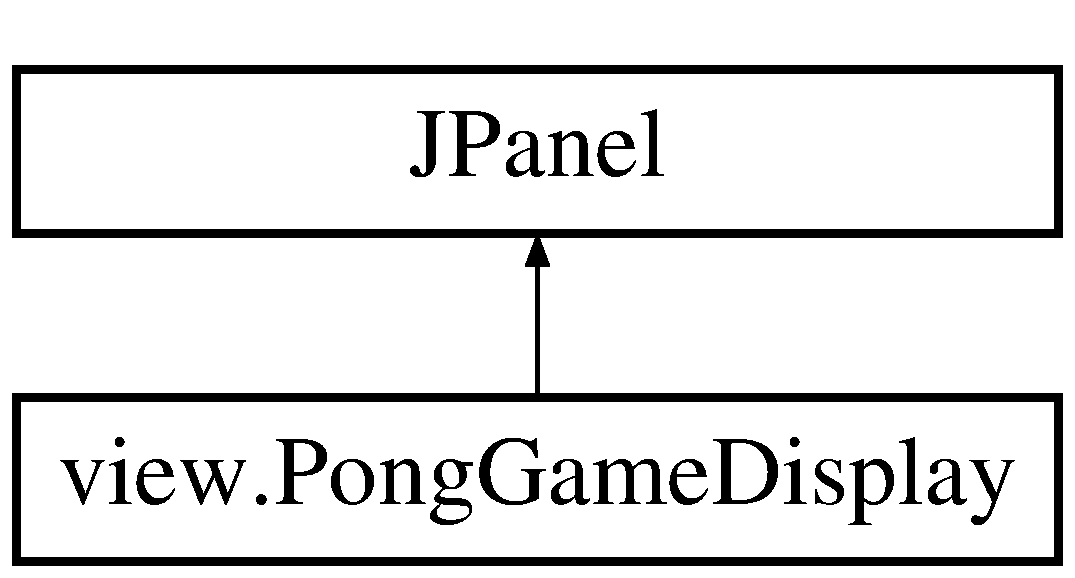
\includegraphics[height=2.000000cm]{classview_1_1_pong_game_display}
\end{center}
\end{figure}
\subsection*{Public Member Functions}
\begin{DoxyCompactItemize}
\item 
\hyperlink{classview_1_1_pong_game_display_a1d578a032b81c4025ba91e6366672e07}{Pong\+Game\+Display} ()
\begin{DoxyCompactList}\small\item\em Constructor for \hyperlink{classview_1_1_pong_game_display}{Pong\+Game\+Display}. \end{DoxyCompactList}\item 
void \hyperlink{classview_1_1_pong_game_display_ac6afa3842b0a26be46dd0b7d202d887d}{set\+Ball} (int x, int y)
\begin{DoxyCompactList}\small\item\em sets the positions of the ball \end{DoxyCompactList}\item 
void \hyperlink{classview_1_1_pong_game_display_aa2f0ba3a3f8bc84bd079302904a57133}{set\+Bottom\+Paddle} (int x, int y)
\item 
void \hyperlink{classview_1_1_pong_game_display_a175282d960f6beec7819bd373f09f170}{set\+Top\+Paddle} (int x, int y)
\item 
void \hyperlink{classview_1_1_pong_game_display_adb358611d0a270aaf5954141ec8d35c0}{set\+Bomb} (int x, int y)
\begin{DoxyCompactList}\small\item\em sets the positions of the bomb \end{DoxyCompactList}\item 
void \hyperlink{classview_1_1_pong_game_display_a67b7b51feffc6573e92ac9c979ade0e2}{time\+For\+Bomb} ()
\begin{DoxyCompactList}\small\item\em defines the game mode contains a bomb \end{DoxyCompactList}\item 
void \hyperlink{classview_1_1_pong_game_display_a51b69bc0f6f840b4c736049115e0f449}{no\+Bomb} ()
\begin{DoxyCompactList}\small\item\em defines the game mode does not contain a bomb \end{DoxyCompactList}\item 
void \hyperlink{classview_1_1_pong_game_display_a295d4a14e718454eb223a5bb06141d53}{set\+Ball\+Size} (int s)
\begin{DoxyCompactList}\small\item\em sets the size of the ball \end{DoxyCompactList}\item 
void \hyperlink{classview_1_1_pong_game_display_aeaaff1c8033efd2d7f3242ab3b6c7e9e}{set\+Bottom} (int x)
\begin{DoxyCompactList}\small\item\em sets x-\/position for the player paddle \end{DoxyCompactList}\item 
void \hyperlink{classview_1_1_pong_game_display_a8b9caa56b471453556b7380ee6d37340}{set\+Top} (int x)
\begin{DoxyCompactList}\small\item\em sets x-\/position for the ai paddle \end{DoxyCompactList}\item 
int \hyperlink{classview_1_1_pong_game_display_ab5d2d9429f7d666fea097c2ea3118893}{get\+BottomX} ()
\begin{DoxyCompactList}\small\item\em gets the x-\/position of the player paddle \end{DoxyCompactList}\item 
int \hyperlink{classview_1_1_pong_game_display_afa4d22c9959dc02057a1b56fef3f33cd}{get\+BottomY} ()
\begin{DoxyCompactList}\small\item\em gets the y-\/position of the player paddle \end{DoxyCompactList}\item 
void \hyperlink{classview_1_1_pong_game_display_a04bcc8b60d85f38178d2cd817e3fbd39}{set\+Top\+Score} (int s)
\begin{DoxyCompactList}\small\item\em sets the score for ai \end{DoxyCompactList}\item 
void \hyperlink{classview_1_1_pong_game_display_aa1ef677f1bae92a51750732099b1609a}{set\+Bottom\+Score} (int s)
\begin{DoxyCompactList}\small\item\em sets the score for player \end{DoxyCompactList}\item 
int \hyperlink{classview_1_1_pong_game_display_a83584a112f5bd8877e1bbb1d74dfa080}{get\+BallX} ()
\begin{DoxyCompactList}\small\item\em gets the x-\/position of the ball \end{DoxyCompactList}\item 
int \hyperlink{classview_1_1_pong_game_display_a940198a68c987548b182d18069ba5885}{get\+BallY} ()
\begin{DoxyCompactList}\small\item\em gets the y-\/position of the ball \end{DoxyCompactList}\item 
void \hyperlink{classview_1_1_pong_game_display_ac42d38f9ed29e2ab2bec6c7da46f1c0e}{set\+Paddle\+Width} (int w)
\begin{DoxyCompactList}\small\item\em sets the width of the paddle \end{DoxyCompactList}\item 
void \hyperlink{classview_1_1_pong_game_display_a5c855e1e459838b82e976cd957da5cc5}{set\+Paddle\+Height} (int h)
\begin{DoxyCompactList}\small\item\em sets the height of the paddle \end{DoxyCompactList}\item 
void \hyperlink{classview_1_1_pong_game_display_ac40ce3811b6118c530980d38aa48ec64}{set\+Inset} (int i)
\begin{DoxyCompactList}\small\item\em sets the distance between frame and the paddle \end{DoxyCompactList}\item 
void \hyperlink{classview_1_1_pong_game_display_a0fedbf41897932915b12f67542cb7695}{set\+Advance} ()
\begin{DoxyCompactList}\small\item\em sets the game mode to be advanced \end{DoxyCompactList}\end{DoxyCompactItemize}
\subsection*{Protected Member Functions}
\begin{DoxyCompactItemize}
\item 
void \hyperlink{classview_1_1_pong_game_display_a0e3a18dfc9bbd76c97439a618a3330ac}{paint\+Component} (Graphics g)
\begin{DoxyCompactList}\small\item\em draws shapes on the screen \end{DoxyCompactList}\end{DoxyCompactItemize}
\subsection*{Private Attributes}
\begin{DoxyCompactItemize}
\item 
int \hyperlink{classview_1_1_pong_game_display_aacbf5c26433ea74107021b461af657c1}{frame\+Width}
\item 
int \hyperlink{classview_1_1_pong_game_display_a1263ea81d63ff3e12b37fee42225a22e}{frame\+Height}
\item 
int \hyperlink{classview_1_1_pong_game_display_a14bdd6ada555582531723e7c11784251}{score\+Top}
\item 
int \hyperlink{classview_1_1_pong_game_display_aa1f518edcfa598a7ba036567eadf3ae0}{ballX}
\item 
int \hyperlink{classview_1_1_pong_game_display_ac37e1767ccd91ae204de6b0afc5aefaa}{bombX}
\item 
int \hyperlink{classview_1_1_pong_game_display_a195949e482e01530f0c8c876bbf88e6a}{bottom\+PadX}
\item 
int \hyperlink{classview_1_1_pong_game_display_a808ad12c167de880ca74e5ad56ea5f43}{top\+PadX}
\item 
boolean \hyperlink{classview_1_1_pong_game_display_aeb378cbf5a0a37e9105c9748910f3513}{first}
\item 
int \hyperlink{classview_1_1_pong_game_display_ae26155e2cdf4f47b164377b7ee3ba3e4}{ball\+Size}
\item 
int \hyperlink{classview_1_1_pong_game_display_a9617cc99b5e08dc62ac3272a0934d576}{padW}
\item 
int \hyperlink{classview_1_1_pong_game_display_ac202bb5082c22fb3f40ddff2ccc797b5}{inset}
\item 
int \hyperlink{classview_1_1_pong_game_display_a38f4635d73ef3c3986ad8a351b6f7a69}{game\+Mode}
\item 
final int \hyperlink{classview_1_1_pong_game_display_a8d4dbbd4e9ba52b12ba951899c7fe02d}{S\+I\+N\+G\+LE} =0
\item 
final int \hyperlink{classview_1_1_pong_game_display_a3aa7541f41ee227f6f7c3acf0bd35871}{A\+D\+V\+A\+N\+CE} =1
\item 
boolean \hyperlink{classview_1_1_pong_game_display_a4acf14f2571c372dd4737fac2b8d7412}{start\+Bomb}
\end{DoxyCompactItemize}


\subsection{Constructor \& Destructor Documentation}
\hypertarget{classview_1_1_pong_game_display_a1d578a032b81c4025ba91e6366672e07}{}\label{classview_1_1_pong_game_display_a1d578a032b81c4025ba91e6366672e07} 
\index{view\+::\+Pong\+Game\+Display@{view\+::\+Pong\+Game\+Display}!Pong\+Game\+Display@{Pong\+Game\+Display}}
\index{Pong\+Game\+Display@{Pong\+Game\+Display}!view\+::\+Pong\+Game\+Display@{view\+::\+Pong\+Game\+Display}}
\subsubsection{\texorpdfstring{Pong\+Game\+Display()}{PongGameDisplay()}}
{\footnotesize\ttfamily view.\+Pong\+Game\+Display.\+Pong\+Game\+Display (\begin{DoxyParamCaption}{ }\end{DoxyParamCaption})}



Constructor for \hyperlink{classview_1_1_pong_game_display}{Pong\+Game\+Display}. 

Constructor by default set the game to single mode 

\subsection{Member Function Documentation}
\hypertarget{classview_1_1_pong_game_display_a83584a112f5bd8877e1bbb1d74dfa080}{}\label{classview_1_1_pong_game_display_a83584a112f5bd8877e1bbb1d74dfa080} 
\index{view\+::\+Pong\+Game\+Display@{view\+::\+Pong\+Game\+Display}!get\+BallX@{get\+BallX}}
\index{get\+BallX@{get\+BallX}!view\+::\+Pong\+Game\+Display@{view\+::\+Pong\+Game\+Display}}
\subsubsection{\texorpdfstring{get\+Ball\+X()}{getBallX()}}
{\footnotesize\ttfamily int view.\+Pong\+Game\+Display.\+get\+BallX (\begin{DoxyParamCaption}{ }\end{DoxyParamCaption})}



gets the x-\/position of the ball 

\begin{DoxyReturn}{Returns}
ballX 
\end{DoxyReturn}
\hypertarget{classview_1_1_pong_game_display_a940198a68c987548b182d18069ba5885}{}\label{classview_1_1_pong_game_display_a940198a68c987548b182d18069ba5885} 
\index{view\+::\+Pong\+Game\+Display@{view\+::\+Pong\+Game\+Display}!get\+BallY@{get\+BallY}}
\index{get\+BallY@{get\+BallY}!view\+::\+Pong\+Game\+Display@{view\+::\+Pong\+Game\+Display}}
\subsubsection{\texorpdfstring{get\+Ball\+Y()}{getBallY()}}
{\footnotesize\ttfamily int view.\+Pong\+Game\+Display.\+get\+BallY (\begin{DoxyParamCaption}{ }\end{DoxyParamCaption})}



gets the y-\/position of the ball 

\begin{DoxyReturn}{Returns}
ballY 
\end{DoxyReturn}
\hypertarget{classview_1_1_pong_game_display_ab5d2d9429f7d666fea097c2ea3118893}{}\label{classview_1_1_pong_game_display_ab5d2d9429f7d666fea097c2ea3118893} 
\index{view\+::\+Pong\+Game\+Display@{view\+::\+Pong\+Game\+Display}!get\+BottomX@{get\+BottomX}}
\index{get\+BottomX@{get\+BottomX}!view\+::\+Pong\+Game\+Display@{view\+::\+Pong\+Game\+Display}}
\subsubsection{\texorpdfstring{get\+Bottom\+X()}{getBottomX()}}
{\footnotesize\ttfamily int view.\+Pong\+Game\+Display.\+get\+BottomX (\begin{DoxyParamCaption}{ }\end{DoxyParamCaption})}



gets the x-\/position of the player paddle 

\begin{DoxyReturn}{Returns}
bottom\+PadX 
\end{DoxyReturn}
\hypertarget{classview_1_1_pong_game_display_afa4d22c9959dc02057a1b56fef3f33cd}{}\label{classview_1_1_pong_game_display_afa4d22c9959dc02057a1b56fef3f33cd} 
\index{view\+::\+Pong\+Game\+Display@{view\+::\+Pong\+Game\+Display}!get\+BottomY@{get\+BottomY}}
\index{get\+BottomY@{get\+BottomY}!view\+::\+Pong\+Game\+Display@{view\+::\+Pong\+Game\+Display}}
\subsubsection{\texorpdfstring{get\+Bottom\+Y()}{getBottomY()}}
{\footnotesize\ttfamily int view.\+Pong\+Game\+Display.\+get\+BottomY (\begin{DoxyParamCaption}{ }\end{DoxyParamCaption})}



gets the y-\/position of the player paddle 

\begin{DoxyReturn}{Returns}
bottom\+PadY 
\end{DoxyReturn}
\hypertarget{classview_1_1_pong_game_display_a51b69bc0f6f840b4c736049115e0f449}{}\label{classview_1_1_pong_game_display_a51b69bc0f6f840b4c736049115e0f449} 
\index{view\+::\+Pong\+Game\+Display@{view\+::\+Pong\+Game\+Display}!no\+Bomb@{no\+Bomb}}
\index{no\+Bomb@{no\+Bomb}!view\+::\+Pong\+Game\+Display@{view\+::\+Pong\+Game\+Display}}
\subsubsection{\texorpdfstring{no\+Bomb()}{noBomb()}}
{\footnotesize\ttfamily void view.\+Pong\+Game\+Display.\+no\+Bomb (\begin{DoxyParamCaption}{ }\end{DoxyParamCaption})}



defines the game mode does not contain a bomb 

set the flag for the advance to be false \hypertarget{classview_1_1_pong_game_display_a0e3a18dfc9bbd76c97439a618a3330ac}{}\label{classview_1_1_pong_game_display_a0e3a18dfc9bbd76c97439a618a3330ac} 
\index{view\+::\+Pong\+Game\+Display@{view\+::\+Pong\+Game\+Display}!paint\+Component@{paint\+Component}}
\index{paint\+Component@{paint\+Component}!view\+::\+Pong\+Game\+Display@{view\+::\+Pong\+Game\+Display}}
\subsubsection{\texorpdfstring{paint\+Component()}{paintComponent()}}
{\footnotesize\ttfamily void view.\+Pong\+Game\+Display.\+paint\+Component (\begin{DoxyParamCaption}\item[{Graphics}]{g }\end{DoxyParamCaption})\hspace{0.3cm}{\ttfamily [protected]}}



draws shapes on the screen 

when the game is started, by default draws the ball and paddles in the middle, otherwise, draws objects by passed in values. Initial positioning
\begin{DoxyItemize}
\item ball at the center of the screen
\item paddle in the middle of the frame width
\end{DoxyItemize}

Draw rectangles by passed in values

Draw the ball by passed in values

Draw the bomb if the mode is the advance mode

Draw scores on the screen by passed in values\hypertarget{classview_1_1_pong_game_display_a0fedbf41897932915b12f67542cb7695}{}\label{classview_1_1_pong_game_display_a0fedbf41897932915b12f67542cb7695} 
\index{view\+::\+Pong\+Game\+Display@{view\+::\+Pong\+Game\+Display}!set\+Advance@{set\+Advance}}
\index{set\+Advance@{set\+Advance}!view\+::\+Pong\+Game\+Display@{view\+::\+Pong\+Game\+Display}}
\subsubsection{\texorpdfstring{set\+Advance()}{setAdvance()}}
{\footnotesize\ttfamily void view.\+Pong\+Game\+Display.\+set\+Advance (\begin{DoxyParamCaption}{ }\end{DoxyParamCaption})}



sets the game mode to be advanced 

set the flag to advance \hypertarget{classview_1_1_pong_game_display_ac6afa3842b0a26be46dd0b7d202d887d}{}\label{classview_1_1_pong_game_display_ac6afa3842b0a26be46dd0b7d202d887d} 
\index{view\+::\+Pong\+Game\+Display@{view\+::\+Pong\+Game\+Display}!set\+Ball@{set\+Ball}}
\index{set\+Ball@{set\+Ball}!view\+::\+Pong\+Game\+Display@{view\+::\+Pong\+Game\+Display}}
\subsubsection{\texorpdfstring{set\+Ball()}{setBall()}}
{\footnotesize\ttfamily void view.\+Pong\+Game\+Display.\+set\+Ball (\begin{DoxyParamCaption}\item[{int}]{x,  }\item[{int}]{y }\end{DoxyParamCaption})}



sets the positions of the ball 


\begin{DoxyParams}{Parameters}
{\em x} & is the x-\/position of the ball \\
\hline
{\em y} & is the y-\/position of the ball \\
\hline
\end{DoxyParams}
\hypertarget{classview_1_1_pong_game_display_a295d4a14e718454eb223a5bb06141d53}{}\label{classview_1_1_pong_game_display_a295d4a14e718454eb223a5bb06141d53} 
\index{view\+::\+Pong\+Game\+Display@{view\+::\+Pong\+Game\+Display}!set\+Ball\+Size@{set\+Ball\+Size}}
\index{set\+Ball\+Size@{set\+Ball\+Size}!view\+::\+Pong\+Game\+Display@{view\+::\+Pong\+Game\+Display}}
\subsubsection{\texorpdfstring{set\+Ball\+Size()}{setBallSize()}}
{\footnotesize\ttfamily void view.\+Pong\+Game\+Display.\+set\+Ball\+Size (\begin{DoxyParamCaption}\item[{int}]{s }\end{DoxyParamCaption})}



sets the size of the ball 


\begin{DoxyParams}{Parameters}
{\em s} & is the ball size \\
\hline
\end{DoxyParams}
\hypertarget{classview_1_1_pong_game_display_adb358611d0a270aaf5954141ec8d35c0}{}\label{classview_1_1_pong_game_display_adb358611d0a270aaf5954141ec8d35c0} 
\index{view\+::\+Pong\+Game\+Display@{view\+::\+Pong\+Game\+Display}!set\+Bomb@{set\+Bomb}}
\index{set\+Bomb@{set\+Bomb}!view\+::\+Pong\+Game\+Display@{view\+::\+Pong\+Game\+Display}}
\subsubsection{\texorpdfstring{set\+Bomb()}{setBomb()}}
{\footnotesize\ttfamily void view.\+Pong\+Game\+Display.\+set\+Bomb (\begin{DoxyParamCaption}\item[{int}]{x,  }\item[{int}]{y }\end{DoxyParamCaption})}



sets the positions of the bomb 


\begin{DoxyParams}{Parameters}
{\em x} & is the x-\/position of the bomb \\
\hline
{\em y} & is the y-\/position of the bomb \\
\hline
\end{DoxyParams}
\hypertarget{classview_1_1_pong_game_display_aeaaff1c8033efd2d7f3242ab3b6c7e9e}{}\label{classview_1_1_pong_game_display_aeaaff1c8033efd2d7f3242ab3b6c7e9e} 
\index{view\+::\+Pong\+Game\+Display@{view\+::\+Pong\+Game\+Display}!set\+Bottom@{set\+Bottom}}
\index{set\+Bottom@{set\+Bottom}!view\+::\+Pong\+Game\+Display@{view\+::\+Pong\+Game\+Display}}
\subsubsection{\texorpdfstring{set\+Bottom()}{setBottom()}}
{\footnotesize\ttfamily void view.\+Pong\+Game\+Display.\+set\+Bottom (\begin{DoxyParamCaption}\item[{int}]{x }\end{DoxyParamCaption})}



sets x-\/position for the player paddle 


\begin{DoxyParams}{Parameters}
{\em s} & is the x-\/position \\
\hline
\end{DoxyParams}
\hypertarget{classview_1_1_pong_game_display_aa2f0ba3a3f8bc84bd079302904a57133}{}\label{classview_1_1_pong_game_display_aa2f0ba3a3f8bc84bd079302904a57133} 
\index{view\+::\+Pong\+Game\+Display@{view\+::\+Pong\+Game\+Display}!set\+Bottom\+Paddle@{set\+Bottom\+Paddle}}
\index{set\+Bottom\+Paddle@{set\+Bottom\+Paddle}!view\+::\+Pong\+Game\+Display@{view\+::\+Pong\+Game\+Display}}
\subsubsection{\texorpdfstring{set\+Bottom\+Paddle()}{setBottomPaddle()}}
{\footnotesize\ttfamily void view.\+Pong\+Game\+Display.\+set\+Bottom\+Paddle (\begin{DoxyParamCaption}\item[{int}]{x,  }\item[{int}]{y }\end{DoxyParamCaption})}

\hypertarget{classview_1_1_pong_game_display_aa1ef677f1bae92a51750732099b1609a}{}\label{classview_1_1_pong_game_display_aa1ef677f1bae92a51750732099b1609a} 
\index{view\+::\+Pong\+Game\+Display@{view\+::\+Pong\+Game\+Display}!set\+Bottom\+Score@{set\+Bottom\+Score}}
\index{set\+Bottom\+Score@{set\+Bottom\+Score}!view\+::\+Pong\+Game\+Display@{view\+::\+Pong\+Game\+Display}}
\subsubsection{\texorpdfstring{set\+Bottom\+Score()}{setBottomScore()}}
{\footnotesize\ttfamily void view.\+Pong\+Game\+Display.\+set\+Bottom\+Score (\begin{DoxyParamCaption}\item[{int}]{s }\end{DoxyParamCaption})}



sets the score for player 


\begin{DoxyParams}{Parameters}
{\em s} & is the score \\
\hline
\end{DoxyParams}
\hypertarget{classview_1_1_pong_game_display_ac40ce3811b6118c530980d38aa48ec64}{}\label{classview_1_1_pong_game_display_ac40ce3811b6118c530980d38aa48ec64} 
\index{view\+::\+Pong\+Game\+Display@{view\+::\+Pong\+Game\+Display}!set\+Inset@{set\+Inset}}
\index{set\+Inset@{set\+Inset}!view\+::\+Pong\+Game\+Display@{view\+::\+Pong\+Game\+Display}}
\subsubsection{\texorpdfstring{set\+Inset()}{setInset()}}
{\footnotesize\ttfamily void view.\+Pong\+Game\+Display.\+set\+Inset (\begin{DoxyParamCaption}\item[{int}]{i }\end{DoxyParamCaption})}



sets the distance between frame and the paddle 


\begin{DoxyParams}{Parameters}
{\em i} & is the inset \\
\hline
\end{DoxyParams}
\hypertarget{classview_1_1_pong_game_display_a5c855e1e459838b82e976cd957da5cc5}{}\label{classview_1_1_pong_game_display_a5c855e1e459838b82e976cd957da5cc5} 
\index{view\+::\+Pong\+Game\+Display@{view\+::\+Pong\+Game\+Display}!set\+Paddle\+Height@{set\+Paddle\+Height}}
\index{set\+Paddle\+Height@{set\+Paddle\+Height}!view\+::\+Pong\+Game\+Display@{view\+::\+Pong\+Game\+Display}}
\subsubsection{\texorpdfstring{set\+Paddle\+Height()}{setPaddleHeight()}}
{\footnotesize\ttfamily void view.\+Pong\+Game\+Display.\+set\+Paddle\+Height (\begin{DoxyParamCaption}\item[{int}]{h }\end{DoxyParamCaption})}



sets the height of the paddle 


\begin{DoxyParams}{Parameters}
{\em h} & is the height \\
\hline
\end{DoxyParams}
\hypertarget{classview_1_1_pong_game_display_ac42d38f9ed29e2ab2bec6c7da46f1c0e}{}\label{classview_1_1_pong_game_display_ac42d38f9ed29e2ab2bec6c7da46f1c0e} 
\index{view\+::\+Pong\+Game\+Display@{view\+::\+Pong\+Game\+Display}!set\+Paddle\+Width@{set\+Paddle\+Width}}
\index{set\+Paddle\+Width@{set\+Paddle\+Width}!view\+::\+Pong\+Game\+Display@{view\+::\+Pong\+Game\+Display}}
\subsubsection{\texorpdfstring{set\+Paddle\+Width()}{setPaddleWidth()}}
{\footnotesize\ttfamily void view.\+Pong\+Game\+Display.\+set\+Paddle\+Width (\begin{DoxyParamCaption}\item[{int}]{w }\end{DoxyParamCaption})}



sets the width of the paddle 


\begin{DoxyParams}{Parameters}
{\em w} & is the width \\
\hline
\end{DoxyParams}
\hypertarget{classview_1_1_pong_game_display_a8b9caa56b471453556b7380ee6d37340}{}\label{classview_1_1_pong_game_display_a8b9caa56b471453556b7380ee6d37340} 
\index{view\+::\+Pong\+Game\+Display@{view\+::\+Pong\+Game\+Display}!set\+Top@{set\+Top}}
\index{set\+Top@{set\+Top}!view\+::\+Pong\+Game\+Display@{view\+::\+Pong\+Game\+Display}}
\subsubsection{\texorpdfstring{set\+Top()}{setTop()}}
{\footnotesize\ttfamily void view.\+Pong\+Game\+Display.\+set\+Top (\begin{DoxyParamCaption}\item[{int}]{x }\end{DoxyParamCaption})}



sets x-\/position for the ai paddle 


\begin{DoxyParams}{Parameters}
{\em s} & is the x-\/position \\
\hline
\end{DoxyParams}
\hypertarget{classview_1_1_pong_game_display_a175282d960f6beec7819bd373f09f170}{}\label{classview_1_1_pong_game_display_a175282d960f6beec7819bd373f09f170} 
\index{view\+::\+Pong\+Game\+Display@{view\+::\+Pong\+Game\+Display}!set\+Top\+Paddle@{set\+Top\+Paddle}}
\index{set\+Top\+Paddle@{set\+Top\+Paddle}!view\+::\+Pong\+Game\+Display@{view\+::\+Pong\+Game\+Display}}
\subsubsection{\texorpdfstring{set\+Top\+Paddle()}{setTopPaddle()}}
{\footnotesize\ttfamily void view.\+Pong\+Game\+Display.\+set\+Top\+Paddle (\begin{DoxyParamCaption}\item[{int}]{x,  }\item[{int}]{y }\end{DoxyParamCaption})}

\hypertarget{classview_1_1_pong_game_display_a04bcc8b60d85f38178d2cd817e3fbd39}{}\label{classview_1_1_pong_game_display_a04bcc8b60d85f38178d2cd817e3fbd39} 
\index{view\+::\+Pong\+Game\+Display@{view\+::\+Pong\+Game\+Display}!set\+Top\+Score@{set\+Top\+Score}}
\index{set\+Top\+Score@{set\+Top\+Score}!view\+::\+Pong\+Game\+Display@{view\+::\+Pong\+Game\+Display}}
\subsubsection{\texorpdfstring{set\+Top\+Score()}{setTopScore()}}
{\footnotesize\ttfamily void view.\+Pong\+Game\+Display.\+set\+Top\+Score (\begin{DoxyParamCaption}\item[{int}]{s }\end{DoxyParamCaption})}



sets the score for ai 


\begin{DoxyParams}{Parameters}
{\em s} & is the score \\
\hline
\end{DoxyParams}
\hypertarget{classview_1_1_pong_game_display_a67b7b51feffc6573e92ac9c979ade0e2}{}\label{classview_1_1_pong_game_display_a67b7b51feffc6573e92ac9c979ade0e2} 
\index{view\+::\+Pong\+Game\+Display@{view\+::\+Pong\+Game\+Display}!time\+For\+Bomb@{time\+For\+Bomb}}
\index{time\+For\+Bomb@{time\+For\+Bomb}!view\+::\+Pong\+Game\+Display@{view\+::\+Pong\+Game\+Display}}
\subsubsection{\texorpdfstring{time\+For\+Bomb()}{timeForBomb()}}
{\footnotesize\ttfamily void view.\+Pong\+Game\+Display.\+time\+For\+Bomb (\begin{DoxyParamCaption}{ }\end{DoxyParamCaption})}



defines the game mode contains a bomb 

set the flag for the advance to be true 

\subsection{Member Data Documentation}
\hypertarget{classview_1_1_pong_game_display_a3aa7541f41ee227f6f7c3acf0bd35871}{}\label{classview_1_1_pong_game_display_a3aa7541f41ee227f6f7c3acf0bd35871} 
\index{view\+::\+Pong\+Game\+Display@{view\+::\+Pong\+Game\+Display}!A\+D\+V\+A\+N\+CE@{A\+D\+V\+A\+N\+CE}}
\index{A\+D\+V\+A\+N\+CE@{A\+D\+V\+A\+N\+CE}!view\+::\+Pong\+Game\+Display@{view\+::\+Pong\+Game\+Display}}
\subsubsection{\texorpdfstring{A\+D\+V\+A\+N\+CE}{ADVANCE}}
{\footnotesize\ttfamily final int view.\+Pong\+Game\+Display.\+A\+D\+V\+A\+N\+CE =1\hspace{0.3cm}{\ttfamily [private]}}

\hypertarget{classview_1_1_pong_game_display_ae26155e2cdf4f47b164377b7ee3ba3e4}{}\label{classview_1_1_pong_game_display_ae26155e2cdf4f47b164377b7ee3ba3e4} 
\index{view\+::\+Pong\+Game\+Display@{view\+::\+Pong\+Game\+Display}!ball\+Size@{ball\+Size}}
\index{ball\+Size@{ball\+Size}!view\+::\+Pong\+Game\+Display@{view\+::\+Pong\+Game\+Display}}
\subsubsection{\texorpdfstring{ball\+Size}{ballSize}}
{\footnotesize\ttfamily int view.\+Pong\+Game\+Display.\+ball\+Size\hspace{0.3cm}{\ttfamily [private]}}

\hypertarget{classview_1_1_pong_game_display_aa1f518edcfa598a7ba036567eadf3ae0}{}\label{classview_1_1_pong_game_display_aa1f518edcfa598a7ba036567eadf3ae0} 
\index{view\+::\+Pong\+Game\+Display@{view\+::\+Pong\+Game\+Display}!ballX@{ballX}}
\index{ballX@{ballX}!view\+::\+Pong\+Game\+Display@{view\+::\+Pong\+Game\+Display}}
\subsubsection{\texorpdfstring{ballX}{ballX}}
{\footnotesize\ttfamily int view.\+Pong\+Game\+Display.\+ballX\hspace{0.3cm}{\ttfamily [private]}}

\hypertarget{classview_1_1_pong_game_display_ac37e1767ccd91ae204de6b0afc5aefaa}{}\label{classview_1_1_pong_game_display_ac37e1767ccd91ae204de6b0afc5aefaa} 
\index{view\+::\+Pong\+Game\+Display@{view\+::\+Pong\+Game\+Display}!bombX@{bombX}}
\index{bombX@{bombX}!view\+::\+Pong\+Game\+Display@{view\+::\+Pong\+Game\+Display}}
\subsubsection{\texorpdfstring{bombX}{bombX}}
{\footnotesize\ttfamily int view.\+Pong\+Game\+Display.\+bombX\hspace{0.3cm}{\ttfamily [private]}}

\hypertarget{classview_1_1_pong_game_display_a195949e482e01530f0c8c876bbf88e6a}{}\label{classview_1_1_pong_game_display_a195949e482e01530f0c8c876bbf88e6a} 
\index{view\+::\+Pong\+Game\+Display@{view\+::\+Pong\+Game\+Display}!bottom\+PadX@{bottom\+PadX}}
\index{bottom\+PadX@{bottom\+PadX}!view\+::\+Pong\+Game\+Display@{view\+::\+Pong\+Game\+Display}}
\subsubsection{\texorpdfstring{bottom\+PadX}{bottomPadX}}
{\footnotesize\ttfamily int view.\+Pong\+Game\+Display.\+bottom\+PadX\hspace{0.3cm}{\ttfamily [private]}}

\hypertarget{classview_1_1_pong_game_display_aeb378cbf5a0a37e9105c9748910f3513}{}\label{classview_1_1_pong_game_display_aeb378cbf5a0a37e9105c9748910f3513} 
\index{view\+::\+Pong\+Game\+Display@{view\+::\+Pong\+Game\+Display}!first@{first}}
\index{first@{first}!view\+::\+Pong\+Game\+Display@{view\+::\+Pong\+Game\+Display}}
\subsubsection{\texorpdfstring{first}{first}}
{\footnotesize\ttfamily boolean view.\+Pong\+Game\+Display.\+first\hspace{0.3cm}{\ttfamily [private]}}

\hypertarget{classview_1_1_pong_game_display_a1263ea81d63ff3e12b37fee42225a22e}{}\label{classview_1_1_pong_game_display_a1263ea81d63ff3e12b37fee42225a22e} 
\index{view\+::\+Pong\+Game\+Display@{view\+::\+Pong\+Game\+Display}!frame\+Height@{frame\+Height}}
\index{frame\+Height@{frame\+Height}!view\+::\+Pong\+Game\+Display@{view\+::\+Pong\+Game\+Display}}
\subsubsection{\texorpdfstring{frame\+Height}{frameHeight}}
{\footnotesize\ttfamily int view.\+Pong\+Game\+Display.\+frame\+Height\hspace{0.3cm}{\ttfamily [private]}}

\hypertarget{classview_1_1_pong_game_display_aacbf5c26433ea74107021b461af657c1}{}\label{classview_1_1_pong_game_display_aacbf5c26433ea74107021b461af657c1} 
\index{view\+::\+Pong\+Game\+Display@{view\+::\+Pong\+Game\+Display}!frame\+Width@{frame\+Width}}
\index{frame\+Width@{frame\+Width}!view\+::\+Pong\+Game\+Display@{view\+::\+Pong\+Game\+Display}}
\subsubsection{\texorpdfstring{frame\+Width}{frameWidth}}
{\footnotesize\ttfamily int view.\+Pong\+Game\+Display.\+frame\+Width\hspace{0.3cm}{\ttfamily [private]}}

Variable declarations for the display
\begin{DoxyItemize}
\item frame dimension
\item ball information
\item bomb information
\item player scores
\item paddle information 
\end{DoxyItemize}\hypertarget{classview_1_1_pong_game_display_a38f4635d73ef3c3986ad8a351b6f7a69}{}\label{classview_1_1_pong_game_display_a38f4635d73ef3c3986ad8a351b6f7a69} 
\index{view\+::\+Pong\+Game\+Display@{view\+::\+Pong\+Game\+Display}!game\+Mode@{game\+Mode}}
\index{game\+Mode@{game\+Mode}!view\+::\+Pong\+Game\+Display@{view\+::\+Pong\+Game\+Display}}
\subsubsection{\texorpdfstring{game\+Mode}{gameMode}}
{\footnotesize\ttfamily int view.\+Pong\+Game\+Display.\+game\+Mode\hspace{0.3cm}{\ttfamily [private]}}

\hypertarget{classview_1_1_pong_game_display_ac202bb5082c22fb3f40ddff2ccc797b5}{}\label{classview_1_1_pong_game_display_ac202bb5082c22fb3f40ddff2ccc797b5} 
\index{view\+::\+Pong\+Game\+Display@{view\+::\+Pong\+Game\+Display}!inset@{inset}}
\index{inset@{inset}!view\+::\+Pong\+Game\+Display@{view\+::\+Pong\+Game\+Display}}
\subsubsection{\texorpdfstring{inset}{inset}}
{\footnotesize\ttfamily int view.\+Pong\+Game\+Display.\+inset\hspace{0.3cm}{\ttfamily [private]}}

\hypertarget{classview_1_1_pong_game_display_a9617cc99b5e08dc62ac3272a0934d576}{}\label{classview_1_1_pong_game_display_a9617cc99b5e08dc62ac3272a0934d576} 
\index{view\+::\+Pong\+Game\+Display@{view\+::\+Pong\+Game\+Display}!padW@{padW}}
\index{padW@{padW}!view\+::\+Pong\+Game\+Display@{view\+::\+Pong\+Game\+Display}}
\subsubsection{\texorpdfstring{padW}{padW}}
{\footnotesize\ttfamily int view.\+Pong\+Game\+Display.\+padW\hspace{0.3cm}{\ttfamily [private]}}

\hypertarget{classview_1_1_pong_game_display_a14bdd6ada555582531723e7c11784251}{}\label{classview_1_1_pong_game_display_a14bdd6ada555582531723e7c11784251} 
\index{view\+::\+Pong\+Game\+Display@{view\+::\+Pong\+Game\+Display}!score\+Top@{score\+Top}}
\index{score\+Top@{score\+Top}!view\+::\+Pong\+Game\+Display@{view\+::\+Pong\+Game\+Display}}
\subsubsection{\texorpdfstring{score\+Top}{scoreTop}}
{\footnotesize\ttfamily int view.\+Pong\+Game\+Display.\+score\+Top\hspace{0.3cm}{\ttfamily [private]}}

\hypertarget{classview_1_1_pong_game_display_a8d4dbbd4e9ba52b12ba951899c7fe02d}{}\label{classview_1_1_pong_game_display_a8d4dbbd4e9ba52b12ba951899c7fe02d} 
\index{view\+::\+Pong\+Game\+Display@{view\+::\+Pong\+Game\+Display}!S\+I\+N\+G\+LE@{S\+I\+N\+G\+LE}}
\index{S\+I\+N\+G\+LE@{S\+I\+N\+G\+LE}!view\+::\+Pong\+Game\+Display@{view\+::\+Pong\+Game\+Display}}
\subsubsection{\texorpdfstring{S\+I\+N\+G\+LE}{SINGLE}}
{\footnotesize\ttfamily final int view.\+Pong\+Game\+Display.\+S\+I\+N\+G\+LE =0\hspace{0.3cm}{\ttfamily [private]}}

\hypertarget{classview_1_1_pong_game_display_a4acf14f2571c372dd4737fac2b8d7412}{}\label{classview_1_1_pong_game_display_a4acf14f2571c372dd4737fac2b8d7412} 
\index{view\+::\+Pong\+Game\+Display@{view\+::\+Pong\+Game\+Display}!start\+Bomb@{start\+Bomb}}
\index{start\+Bomb@{start\+Bomb}!view\+::\+Pong\+Game\+Display@{view\+::\+Pong\+Game\+Display}}
\subsubsection{\texorpdfstring{start\+Bomb}{startBomb}}
{\footnotesize\ttfamily boolean view.\+Pong\+Game\+Display.\+start\+Bomb\hspace{0.3cm}{\ttfamily [private]}}

\hypertarget{classview_1_1_pong_game_display_a808ad12c167de880ca74e5ad56ea5f43}{}\label{classview_1_1_pong_game_display_a808ad12c167de880ca74e5ad56ea5f43} 
\index{view\+::\+Pong\+Game\+Display@{view\+::\+Pong\+Game\+Display}!top\+PadX@{top\+PadX}}
\index{top\+PadX@{top\+PadX}!view\+::\+Pong\+Game\+Display@{view\+::\+Pong\+Game\+Display}}
\subsubsection{\texorpdfstring{top\+PadX}{topPadX}}
{\footnotesize\ttfamily int view.\+Pong\+Game\+Display.\+top\+PadX\hspace{0.3cm}{\ttfamily [private]}}



The documentation for this class was generated from the following file\+:\begin{DoxyCompactItemize}
\item 
src/view/\hyperlink{_pong_game_display_8java}{Pong\+Game\+Display.\+java}\end{DoxyCompactItemize}

\hypertarget{classview_1_1_tutorial}{}\section{view.\+Tutorial Class Reference}
\label{classview_1_1_tutorial}\index{view.\+Tutorial@{view.\+Tutorial}}
Inheritance diagram for view.\+Tutorial\+:\begin{figure}[H]
\begin{center}
\leavevmode
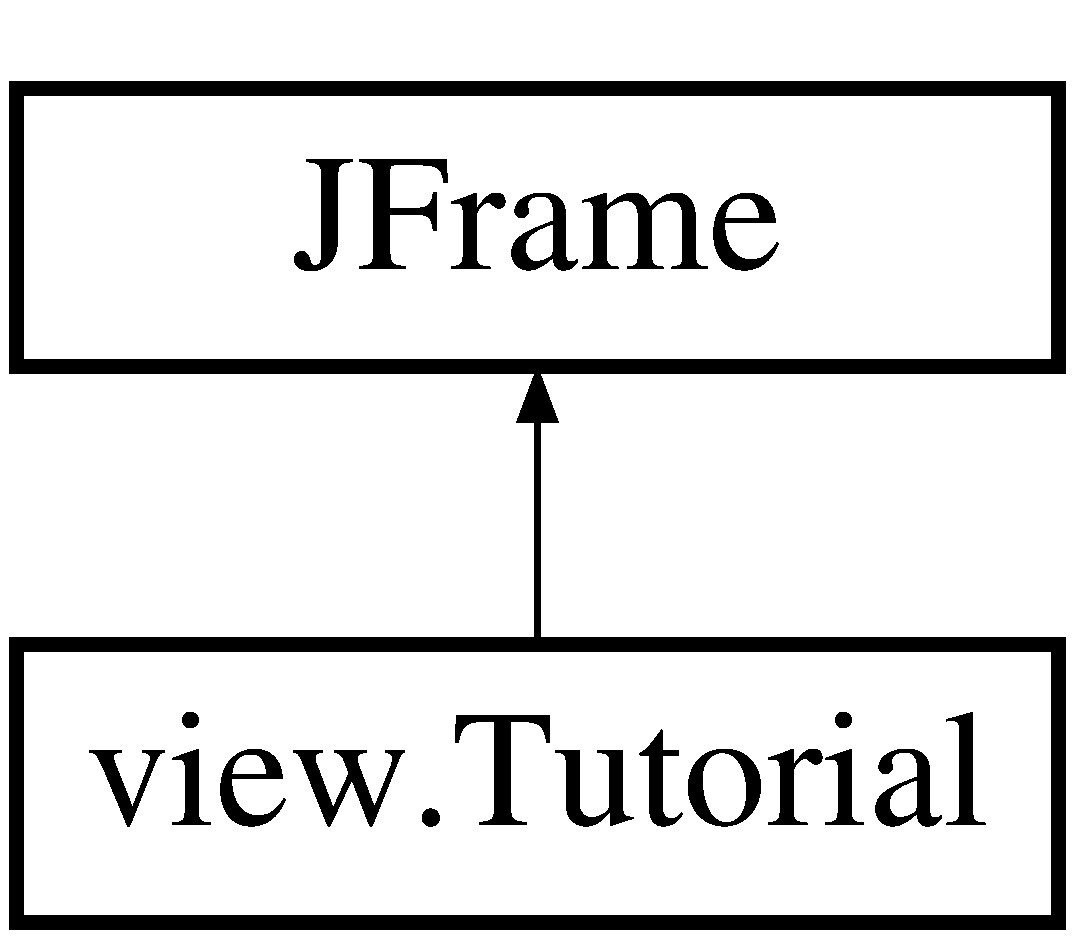
\includegraphics[height=2.000000cm]{classview_1_1_tutorial}
\end{center}
\end{figure}
\subsection*{Public Member Functions}
\begin{DoxyCompactItemize}
\item 
\hyperlink{classview_1_1_tutorial_a0b4dd05d8cf555062780668eb39b9c10}{Tutorial} (Image\+Icon img)
\begin{DoxyCompactList}\small\item\em Constructor for the tutorial page. \end{DoxyCompactList}\item 
J\+Button \hyperlink{classview_1_1_tutorial_a612e0c4badab0a67e6e79364552b452b}{get\+Back} ()
\begin{DoxyCompactList}\small\item\em gets the button to exit the page \end{DoxyCompactList}\item 
void \hyperlink{classview_1_1_tutorial_ab7c6fa062c2541f1b02f1c31f8043811}{add\+Listener} (Action\+Listener listener)
\begin{DoxyCompactList}\small\item\em adds action listener to the button \end{DoxyCompactList}\end{DoxyCompactItemize}
\subsection*{Private Attributes}
\begin{DoxyCompactItemize}
\item 
J\+Button \hyperlink{classview_1_1_tutorial_a9b4a9e5388de99525cc3a982a606ea84}{back}
\end{DoxyCompactItemize}


\subsection{Constructor \& Destructor Documentation}
\hypertarget{classview_1_1_tutorial_a0b4dd05d8cf555062780668eb39b9c10}{}\label{classview_1_1_tutorial_a0b4dd05d8cf555062780668eb39b9c10} 
\index{view\+::\+Tutorial@{view\+::\+Tutorial}!Tutorial@{Tutorial}}
\index{Tutorial@{Tutorial}!view\+::\+Tutorial@{view\+::\+Tutorial}}
\subsubsection{\texorpdfstring{Tutorial()}{Tutorial()}}
{\footnotesize\ttfamily view.\+Tutorial.\+Tutorial (\begin{DoxyParamCaption}\item[{Image\+Icon}]{img }\end{DoxyParamCaption})}



Constructor for the tutorial page. 


\begin{DoxyParams}{Parameters}
{\em img} & is the image for display \\
\hline
\end{DoxyParams}
Setups for the window

Add the image to the window

\subsection{Member Function Documentation}
\hypertarget{classview_1_1_tutorial_ab7c6fa062c2541f1b02f1c31f8043811}{}\label{classview_1_1_tutorial_ab7c6fa062c2541f1b02f1c31f8043811} 
\index{view\+::\+Tutorial@{view\+::\+Tutorial}!add\+Listener@{add\+Listener}}
\index{add\+Listener@{add\+Listener}!view\+::\+Tutorial@{view\+::\+Tutorial}}
\subsubsection{\texorpdfstring{add\+Listener()}{addListener()}}
{\footnotesize\ttfamily void view.\+Tutorial.\+add\+Listener (\begin{DoxyParamCaption}\item[{Action\+Listener}]{listener }\end{DoxyParamCaption})}



adds action listener to the button 


\begin{DoxyParams}{Parameters}
{\em listener} & is the action listener \\
\hline
\end{DoxyParams}
\hypertarget{classview_1_1_tutorial_a612e0c4badab0a67e6e79364552b452b}{}\label{classview_1_1_tutorial_a612e0c4badab0a67e6e79364552b452b} 
\index{view\+::\+Tutorial@{view\+::\+Tutorial}!get\+Back@{get\+Back}}
\index{get\+Back@{get\+Back}!view\+::\+Tutorial@{view\+::\+Tutorial}}
\subsubsection{\texorpdfstring{get\+Back()}{getBack()}}
{\footnotesize\ttfamily J\+Button view.\+Tutorial.\+get\+Back (\begin{DoxyParamCaption}{ }\end{DoxyParamCaption})}



gets the button to exit the page 

\begin{DoxyReturn}{Returns}
back is the button for going back to welcome page 
\end{DoxyReturn}


\subsection{Member Data Documentation}
\hypertarget{classview_1_1_tutorial_a9b4a9e5388de99525cc3a982a606ea84}{}\label{classview_1_1_tutorial_a9b4a9e5388de99525cc3a982a606ea84} 
\index{view\+::\+Tutorial@{view\+::\+Tutorial}!back@{back}}
\index{back@{back}!view\+::\+Tutorial@{view\+::\+Tutorial}}
\subsubsection{\texorpdfstring{back}{back}}
{\footnotesize\ttfamily J\+Button view.\+Tutorial.\+back\hspace{0.3cm}{\ttfamily [private]}}

Variable declaration for the back button 

The documentation for this class was generated from the following file\+:\begin{DoxyCompactItemize}
\item 
src/view/\hyperlink{_tutorial_8java}{Tutorial.\+java}\end{DoxyCompactItemize}

\hypertarget{classview_1_1_welcome}{}\section{view.\+Welcome Class Reference}
\label{classview_1_1_welcome}\index{view.\+Welcome@{view.\+Welcome}}
Inheritance diagram for view.\+Welcome\+:\begin{figure}[H]
\begin{center}
\leavevmode
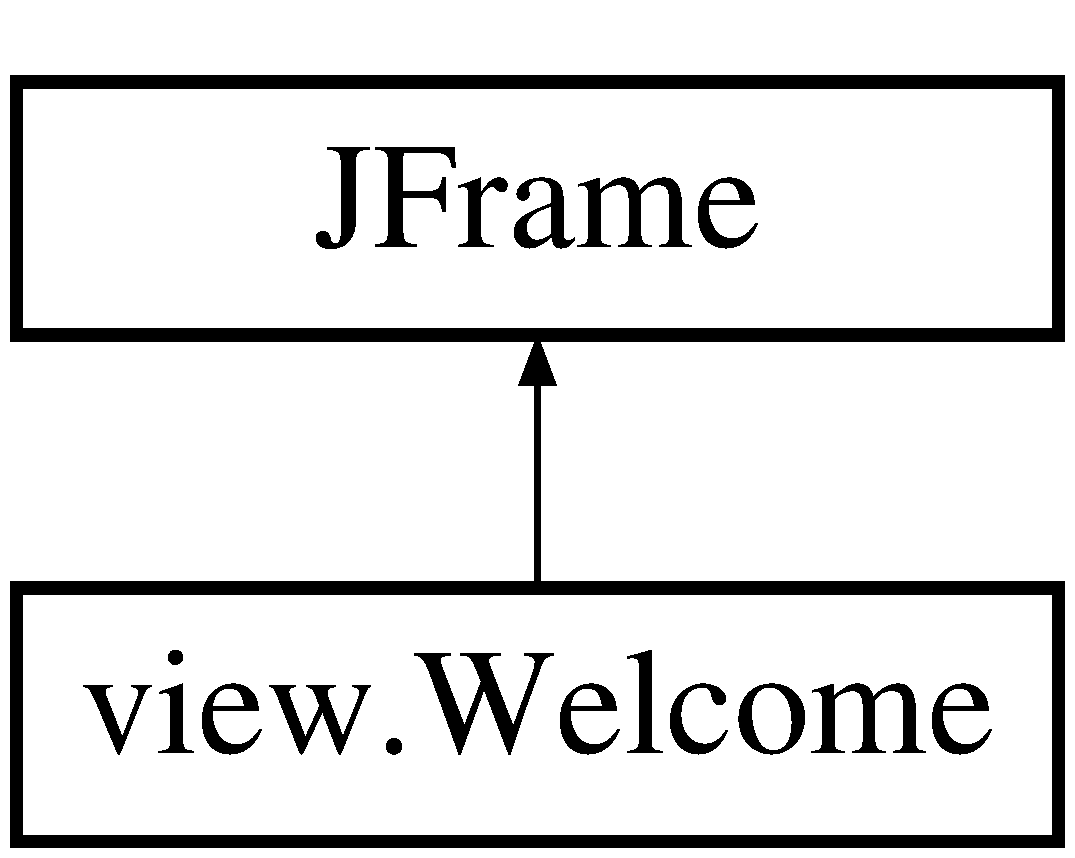
\includegraphics[height=2.000000cm]{classview_1_1_welcome}
\end{center}
\end{figure}
\subsection*{Public Member Functions}
\begin{DoxyCompactItemize}
\item 
\hyperlink{classview_1_1_welcome_ac0d0158b691ccb4dbca2c78145e4a522}{Welcome} ()
\begin{DoxyCompactList}\small\item\em Constructor for welcome page. \end{DoxyCompactList}\item 
J\+Button \hyperlink{classview_1_1_welcome_a8375f9965fb6662e612ea02af51a51a9}{get\+Start} ()
\begin{DoxyCompactList}\small\item\em gets the start button \end{DoxyCompactList}\item 
J\+Button \hyperlink{classview_1_1_welcome_a4a6c30be81cc7a3b081d3e97a4c84356}{load} ()
\begin{DoxyCompactList}\small\item\em gets the load button \end{DoxyCompactList}\item 
J\+Button \hyperlink{classview_1_1_welcome_a5d23e93f1a81a2520d5635ed7d8d5920}{high\+Scores} ()
\begin{DoxyCompactList}\small\item\em gets the button to display high score \end{DoxyCompactList}\item 
J\+Button \hyperlink{classview_1_1_welcome_aaf45e35ac75c1b6f8badd358dd2c2a08}{tutorial} ()
\begin{DoxyCompactList}\small\item\em gets the button to display instructions \end{DoxyCompactList}\item 
J\+Button \hyperlink{classview_1_1_welcome_a78b2940bddd27a89b9462192cbdeaa65}{exit} ()
\begin{DoxyCompactList}\small\item\em gets the button to exit the program \end{DoxyCompactList}\item 
void \hyperlink{classview_1_1_welcome_ac3a30d95eef91daa1df45ccc57d05740}{add\+Button} (J\+Button x)
\begin{DoxyCompactList}\small\item\em adds buttons to a panel \end{DoxyCompactList}\item 
void \hyperlink{classview_1_1_welcome_a0c375320c2042a198ef09c6b8f489ccf}{add\+Listener} (Action\+Listener button\+Listener)
\begin{DoxyCompactList}\small\item\em adds action listener to the buttons \end{DoxyCompactList}\end{DoxyCompactItemize}
\subsection*{Private Attributes}
\begin{DoxyCompactItemize}
\item 
J\+Button \hyperlink{classview_1_1_welcome_a3dfa36fd5db2280f2a2638bacf2d4155}{start} = new J\+Button(\char`\"{}Start New Game\char`\"{})
\item 
J\+Button \hyperlink{classview_1_1_welcome_a91a24fdd828b87e1307d4af30693401e}{load} = new J\+Button(\char`\"{}Load Game\char`\"{})
\item 
J\+Button \hyperlink{classview_1_1_welcome_a824f339b982b2e96f4c6b86287154c5a}{high\+Scores} = new J\+Button(\char`\"{}High Scores\char`\"{})
\item 
J\+Button \hyperlink{classview_1_1_welcome_a8fae2e33d73c97d4bbcc331f050bd68c}{tutorial} = new J\+Button(\char`\"{}Tutorial\char`\"{})
\item 
J\+Button \hyperlink{classview_1_1_welcome_a5a1ae16f7fb3b7f271353133e58bda15}{exit} = new J\+Button(\char`\"{}Exit\char`\"{})
\item 
J\+Panel \hyperlink{classview_1_1_welcome_a846eb5f76566811de2fb852412fb56dc}{button\+Panel}
\end{DoxyCompactItemize}


\subsection{Constructor \& Destructor Documentation}
\hypertarget{classview_1_1_welcome_ac0d0158b691ccb4dbca2c78145e4a522}{}\label{classview_1_1_welcome_ac0d0158b691ccb4dbca2c78145e4a522} 
\index{view\+::\+Welcome@{view\+::\+Welcome}!Welcome@{Welcome}}
\index{Welcome@{Welcome}!view\+::\+Welcome@{view\+::\+Welcome}}
\subsubsection{\texorpdfstring{Welcome()}{Welcome()}}
{\footnotesize\ttfamily view.\+Welcome.\+Welcome (\begin{DoxyParamCaption}{ }\end{DoxyParamCaption})}



Constructor for welcome page. 

sets the header and size of window, and add buttons to it. 
\begin{DoxyItemize}
\item Set the header of the window
\item Set the size of the window
\end{DoxyItemize}

Add buttons on the window

\subsection{Member Function Documentation}
\hypertarget{classview_1_1_welcome_ac3a30d95eef91daa1df45ccc57d05740}{}\label{classview_1_1_welcome_ac3a30d95eef91daa1df45ccc57d05740} 
\index{view\+::\+Welcome@{view\+::\+Welcome}!add\+Button@{add\+Button}}
\index{add\+Button@{add\+Button}!view\+::\+Welcome@{view\+::\+Welcome}}
\subsubsection{\texorpdfstring{add\+Button()}{addButton()}}
{\footnotesize\ttfamily void view.\+Welcome.\+add\+Button (\begin{DoxyParamCaption}\item[{J\+Button}]{x }\end{DoxyParamCaption})}



adds buttons to a panel 

makes buttons align in the panel \hypertarget{classview_1_1_welcome_a0c375320c2042a198ef09c6b8f489ccf}{}\label{classview_1_1_welcome_a0c375320c2042a198ef09c6b8f489ccf} 
\index{view\+::\+Welcome@{view\+::\+Welcome}!add\+Listener@{add\+Listener}}
\index{add\+Listener@{add\+Listener}!view\+::\+Welcome@{view\+::\+Welcome}}
\subsubsection{\texorpdfstring{add\+Listener()}{addListener()}}
{\footnotesize\ttfamily void view.\+Welcome.\+add\+Listener (\begin{DoxyParamCaption}\item[{Action\+Listener}]{button\+Listener }\end{DoxyParamCaption})}



adds action listener to the buttons 


\begin{DoxyParams}{Parameters}
{\em button\+Listener} & is the action listener \\
\hline
\end{DoxyParams}
\hypertarget{classview_1_1_welcome_a78b2940bddd27a89b9462192cbdeaa65}{}\label{classview_1_1_welcome_a78b2940bddd27a89b9462192cbdeaa65} 
\index{view\+::\+Welcome@{view\+::\+Welcome}!exit@{exit}}
\index{exit@{exit}!view\+::\+Welcome@{view\+::\+Welcome}}
\subsubsection{\texorpdfstring{exit()}{exit()}}
{\footnotesize\ttfamily J\+Button view.\+Welcome.\+exit (\begin{DoxyParamCaption}{ }\end{DoxyParamCaption})}



gets the button to exit the program 

\begin{DoxyReturn}{Returns}
exit 
\end{DoxyReturn}
\hypertarget{classview_1_1_welcome_a8375f9965fb6662e612ea02af51a51a9}{}\label{classview_1_1_welcome_a8375f9965fb6662e612ea02af51a51a9} 
\index{view\+::\+Welcome@{view\+::\+Welcome}!get\+Start@{get\+Start}}
\index{get\+Start@{get\+Start}!view\+::\+Welcome@{view\+::\+Welcome}}
\subsubsection{\texorpdfstring{get\+Start()}{getStart()}}
{\footnotesize\ttfamily J\+Button view.\+Welcome.\+get\+Start (\begin{DoxyParamCaption}{ }\end{DoxyParamCaption})}



gets the start button 

\begin{DoxyReturn}{Returns}
start indicates to start a new game 
\end{DoxyReturn}
\hypertarget{classview_1_1_welcome_a5d23e93f1a81a2520d5635ed7d8d5920}{}\label{classview_1_1_welcome_a5d23e93f1a81a2520d5635ed7d8d5920} 
\index{view\+::\+Welcome@{view\+::\+Welcome}!high\+Scores@{high\+Scores}}
\index{high\+Scores@{high\+Scores}!view\+::\+Welcome@{view\+::\+Welcome}}
\subsubsection{\texorpdfstring{high\+Scores()}{highScores()}}
{\footnotesize\ttfamily J\+Button view.\+Welcome.\+high\+Scores (\begin{DoxyParamCaption}{ }\end{DoxyParamCaption})}



gets the button to display high score 

\begin{DoxyReturn}{Returns}
high\+Scores 
\end{DoxyReturn}
\hypertarget{classview_1_1_welcome_a4a6c30be81cc7a3b081d3e97a4c84356}{}\label{classview_1_1_welcome_a4a6c30be81cc7a3b081d3e97a4c84356} 
\index{view\+::\+Welcome@{view\+::\+Welcome}!load@{load}}
\index{load@{load}!view\+::\+Welcome@{view\+::\+Welcome}}
\subsubsection{\texorpdfstring{load()}{load()}}
{\footnotesize\ttfamily J\+Button view.\+Welcome.\+load (\begin{DoxyParamCaption}{ }\end{DoxyParamCaption})}



gets the load button 

\begin{DoxyReturn}{Returns}
load indicates to load a new game 
\end{DoxyReturn}
\hypertarget{classview_1_1_welcome_aaf45e35ac75c1b6f8badd358dd2c2a08}{}\label{classview_1_1_welcome_aaf45e35ac75c1b6f8badd358dd2c2a08} 
\index{view\+::\+Welcome@{view\+::\+Welcome}!tutorial@{tutorial}}
\index{tutorial@{tutorial}!view\+::\+Welcome@{view\+::\+Welcome}}
\subsubsection{\texorpdfstring{tutorial()}{tutorial()}}
{\footnotesize\ttfamily J\+Button view.\+Welcome.\+tutorial (\begin{DoxyParamCaption}{ }\end{DoxyParamCaption})}



gets the button to display instructions 

\begin{DoxyReturn}{Returns}
tutorial 
\end{DoxyReturn}


\subsection{Member Data Documentation}
\hypertarget{classview_1_1_welcome_a846eb5f76566811de2fb852412fb56dc}{}\label{classview_1_1_welcome_a846eb5f76566811de2fb852412fb56dc} 
\index{view\+::\+Welcome@{view\+::\+Welcome}!button\+Panel@{button\+Panel}}
\index{button\+Panel@{button\+Panel}!view\+::\+Welcome@{view\+::\+Welcome}}
\subsubsection{\texorpdfstring{button\+Panel}{buttonPanel}}
{\footnotesize\ttfamily J\+Panel view.\+Welcome.\+button\+Panel\hspace{0.3cm}{\ttfamily [private]}}

Define a panel for the arrangement of buttons \hypertarget{classview_1_1_welcome_a5a1ae16f7fb3b7f271353133e58bda15}{}\label{classview_1_1_welcome_a5a1ae16f7fb3b7f271353133e58bda15} 
\index{view\+::\+Welcome@{view\+::\+Welcome}!exit@{exit}}
\index{exit@{exit}!view\+::\+Welcome@{view\+::\+Welcome}}
\subsubsection{\texorpdfstring{exit}{exit}}
{\footnotesize\ttfamily J\+Button view.\+Welcome.\+exit = new J\+Button(\char`\"{}Exit\char`\"{})\hspace{0.3cm}{\ttfamily [private]}}

\hypertarget{classview_1_1_welcome_a824f339b982b2e96f4c6b86287154c5a}{}\label{classview_1_1_welcome_a824f339b982b2e96f4c6b86287154c5a} 
\index{view\+::\+Welcome@{view\+::\+Welcome}!high\+Scores@{high\+Scores}}
\index{high\+Scores@{high\+Scores}!view\+::\+Welcome@{view\+::\+Welcome}}
\subsubsection{\texorpdfstring{high\+Scores}{highScores}}
{\footnotesize\ttfamily J\+Button view.\+Welcome.\+high\+Scores = new J\+Button(\char`\"{}High Scores\char`\"{})\hspace{0.3cm}{\ttfamily [private]}}

\hypertarget{classview_1_1_welcome_a91a24fdd828b87e1307d4af30693401e}{}\label{classview_1_1_welcome_a91a24fdd828b87e1307d4af30693401e} 
\index{view\+::\+Welcome@{view\+::\+Welcome}!load@{load}}
\index{load@{load}!view\+::\+Welcome@{view\+::\+Welcome}}
\subsubsection{\texorpdfstring{load}{load}}
{\footnotesize\ttfamily J\+Button view.\+Welcome.\+load = new J\+Button(\char`\"{}Load Game\char`\"{})\hspace{0.3cm}{\ttfamily [private]}}

\hypertarget{classview_1_1_welcome_a3dfa36fd5db2280f2a2638bacf2d4155}{}\label{classview_1_1_welcome_a3dfa36fd5db2280f2a2638bacf2d4155} 
\index{view\+::\+Welcome@{view\+::\+Welcome}!start@{start}}
\index{start@{start}!view\+::\+Welcome@{view\+::\+Welcome}}
\subsubsection{\texorpdfstring{start}{start}}
{\footnotesize\ttfamily J\+Button view.\+Welcome.\+start = new J\+Button(\char`\"{}Start New Game\char`\"{})\hspace{0.3cm}{\ttfamily [private]}}

Variable declarations for the page
\begin{DoxyItemize}
\item start a new game
\item load the previous game
\item display high score
\item tutorial
\item exit the game 
\end{DoxyItemize}\hypertarget{classview_1_1_welcome_a8fae2e33d73c97d4bbcc331f050bd68c}{}\label{classview_1_1_welcome_a8fae2e33d73c97d4bbcc331f050bd68c} 
\index{view\+::\+Welcome@{view\+::\+Welcome}!tutorial@{tutorial}}
\index{tutorial@{tutorial}!view\+::\+Welcome@{view\+::\+Welcome}}
\subsubsection{\texorpdfstring{tutorial}{tutorial}}
{\footnotesize\ttfamily J\+Button view.\+Welcome.\+tutorial = new J\+Button(\char`\"{}Tutorial\char`\"{})\hspace{0.3cm}{\ttfamily [private]}}



The documentation for this class was generated from the following file\+:\begin{DoxyCompactItemize}
\item 
src/view/\hyperlink{_welcome_8java}{Welcome.\+java}\end{DoxyCompactItemize}

\chapter{File Documentation}
\hypertarget{_ball_8java}{}\section{src/model/\+Ball.java File Reference}
\label{_ball_8java}\index{src/model/\+Ball.\+java@{src/model/\+Ball.\+java}}


This class represents a ball on the pong game.  


\subsection*{Classes}
\begin{DoxyCompactItemize}
\item 
class \hyperlink{classmodel_1_1_ball}{model.\+Ball}
\end{DoxyCompactItemize}
\subsection*{Packages}
\begin{DoxyCompactItemize}
\item 
package \hyperlink{namespacemodel}{model}
\end{DoxyCompactItemize}


\subsection{Detailed Description}
This class represents a ball on the pong game. 

Ball \begin{DoxyAuthor}{Author}
Pongthusiastics 
\end{DoxyAuthor}
\begin{DoxyDate}{Date}
13/11/2016
\end{DoxyDate}
This class saves the information of a ball, including its position, size and the speed. 
\hypertarget{_game_model_8java}{}\section{src/model/\+Game\+Model.java File Reference}
\label{_game_model_8java}\index{src/model/\+Game\+Model.\+java@{src/model/\+Game\+Model.\+java}}


This class represents a ball on the pong game.  


\subsection*{Classes}
\begin{DoxyCompactItemize}
\item 
class \hyperlink{classmodel_1_1_game_model}{model.\+Game\+Model}
\end{DoxyCompactItemize}
\subsection*{Packages}
\begin{DoxyCompactItemize}
\item 
package \hyperlink{namespacemodel}{model}
\end{DoxyCompactItemize}


\subsection{Detailed Description}
This class represents a ball on the pong game. 

Game\+Model \begin{DoxyAuthor}{Author}
Pongthusiastics 
\end{DoxyAuthor}
\begin{DoxyDate}{Date}
13/11/2016
\end{DoxyDate}
This class saves the information of a ball, including its position, size and the speed. 
\hypertarget{_paddle_8java}{}\section{src/model/\+Paddle.java File Reference}
\label{_paddle_8java}\index{src/model/\+Paddle.\+java@{src/model/\+Paddle.\+java}}


This class defines a paddle.  


\subsection*{Classes}
\begin{DoxyCompactItemize}
\item 
class \hyperlink{classmodel_1_1_paddle}{model.\+Paddle}
\end{DoxyCompactItemize}
\subsection*{Packages}
\begin{DoxyCompactItemize}
\item 
package \hyperlink{namespacemodel}{model}
\end{DoxyCompactItemize}


\subsection{Detailed Description}
This class defines a paddle. 

Paddle \begin{DoxyAuthor}{Author}
Pongthusiastics 
\end{DoxyAuthor}
\begin{DoxyDate}{Date}
13/11/2016
\end{DoxyDate}
This class saves the information of a paddle, including its position, height, width, and inset between the paddle and the screen. 
\hypertarget{_player_8java}{}\section{src/model/\+Player.java File Reference}
\label{_player_8java}\index{src/model/\+Player.\+java@{src/model/\+Player.\+java}}


This class represents a player for the game.  


\subsection*{Classes}
\begin{DoxyCompactItemize}
\item 
class \hyperlink{classmodel_1_1_player}{model.\+Player}
\end{DoxyCompactItemize}
\subsection*{Packages}
\begin{DoxyCompactItemize}
\item 
package \hyperlink{namespacemodel}{model}
\end{DoxyCompactItemize}


\subsection{Detailed Description}
This class represents a player for the game. 

Player \begin{DoxyAuthor}{Author}
Pongthusiastics 
\end{DoxyAuthor}
\begin{DoxyDate}{Date}
13/11/2016
\end{DoxyDate}
This class contains the information for a player, including number of life and his/her current score. 
\hypertarget{_game_controller_8java}{}\section{src/start\+Game/\+Game\+Controller.java File Reference}
\label{_game_controller_8java}\index{src/start\+Game/\+Game\+Controller.\+java@{src/start\+Game/\+Game\+Controller.\+java}}


This class is the controller for the game.  


\subsection*{Classes}
\begin{DoxyCompactItemize}
\item 
class \hyperlink{classstart_game_1_1_game_controller}{start\+Game.\+Game\+Controller}
\item 
class {\bfseries start\+Game.\+Game\+Controller.\+Welcomepage\+Listener}
\begin{DoxyCompactList}\small\item\em action listener for the welcome page \end{DoxyCompactList}\item 
class {\bfseries start\+Game.\+Game\+Controller.\+Mode\+Listener}
\begin{DoxyCompactList}\small\item\em action listener for the game mode page \end{DoxyCompactList}\item 
class {\bfseries start\+Game.\+Game\+Controller.\+Tutorial\+Listener}
\begin{DoxyCompactList}\small\item\em action listener for the tutorial page \end{DoxyCompactList}\item 
class {\bfseries start\+Game.\+Game\+Controller.\+Game\+Listener}
\begin{DoxyCompactList}\small\item\em action listener for the game page \end{DoxyCompactList}\end{DoxyCompactItemize}
\subsection*{Packages}
\begin{DoxyCompactItemize}
\item 
package \hyperlink{namespacestart_game}{start\+Game}
\end{DoxyCompactItemize}


\subsection{Detailed Description}
This class is the controller for the game. 

Game\+Controller \begin{DoxyAuthor}{Author}
Pongthusiastics 
\end{DoxyAuthor}
\begin{DoxyDate}{Date}
13/11/2016
\end{DoxyDate}
This class cooperates with model and view and give direction to the game. 
\hypertarget{_pong_game_8java}{}\section{src/start\+Game/\+Pong\+Game.java File Reference}
\label{_pong_game_8java}\index{src/start\+Game/\+Pong\+Game.\+java@{src/start\+Game/\+Pong\+Game.\+java}}


This class starts the game.  


\subsection*{Classes}
\begin{DoxyCompactItemize}
\item 
class \hyperlink{classstart_game_1_1_pong_game}{start\+Game.\+Pong\+Game}
\end{DoxyCompactItemize}
\subsection*{Packages}
\begin{DoxyCompactItemize}
\item 
package \hyperlink{namespacestart_game}{start\+Game}
\end{DoxyCompactItemize}


\subsection{Detailed Description}
This class starts the game. 

Pong\+Game \begin{DoxyAuthor}{Author}
Pongthusiastics 
\end{DoxyAuthor}
\begin{DoxyDate}{Date}
13/11/2016
\end{DoxyDate}
This class instantiates a model, view, and controller using the M\+VC model, and starts the game. 
\begin{DoxyCode}
GameView \hyperlink{namespaceview}{view} = \textcolor{keyword}{new} GameView();
GameModel \hyperlink{namespacemodel}{model} = \textcolor{keyword}{new} GameModel();
GameController controller = \textcolor{keyword}{new} GameController(view, model);
controller.display();
\end{DoxyCode}
 
\hypertarget{_game_view_8java}{}\section{src/view/\+Game\+View.java File Reference}
\label{_game_view_8java}\index{src/view/\+Game\+View.\+java@{src/view/\+Game\+View.\+java}}


This class is the main view model.  


\subsection*{Classes}
\begin{DoxyCompactItemize}
\item 
class \hyperlink{classview_1_1_game_view}{view.\+Game\+View}
\end{DoxyCompactItemize}
\subsection*{Packages}
\begin{DoxyCompactItemize}
\item 
package \hyperlink{namespaceview}{view}
\end{DoxyCompactItemize}


\subsection{Detailed Description}
This class is the main view model. 

Game\+View \begin{DoxyAuthor}{Author}
Pongthusiastics 
\end{DoxyAuthor}
\begin{DoxyDate}{Date}
13/11/2016
\end{DoxyDate}
This class import all different windows for display. 
\hypertarget{_mode_8java}{}\section{src/view/\+Mode.java File Reference}
\label{_mode_8java}\index{src/view/\+Mode.\+java@{src/view/\+Mode.\+java}}


This class create the game mode window.  


\subsection*{Classes}
\begin{DoxyCompactItemize}
\item 
class \hyperlink{classview_1_1_mode}{view.\+Mode}
\end{DoxyCompactItemize}
\subsection*{Packages}
\begin{DoxyCompactItemize}
\item 
package \hyperlink{namespaceview}{view}
\end{DoxyCompactItemize}


\subsection{Detailed Description}
This class create the game mode window. 

Mode \begin{DoxyAuthor}{Author}
Pongthusiastics 
\end{DoxyAuthor}
\begin{DoxyDate}{Date}
13/11/2016
\end{DoxyDate}
This class create a frame and buttons for different game level 
\hypertarget{_pong_game_display_8java}{}\section{src/view/\+Pong\+Game\+Display.java File Reference}
\label{_pong_game_display_8java}\index{src/view/\+Pong\+Game\+Display.\+java@{src/view/\+Pong\+Game\+Display.\+java}}


This class construct the view of the pong game.  


\subsection*{Classes}
\begin{DoxyCompactItemize}
\item 
class \hyperlink{classview_1_1_pong_game_display}{view.\+Pong\+Game\+Display}
\end{DoxyCompactItemize}
\subsection*{Packages}
\begin{DoxyCompactItemize}
\item 
package \hyperlink{namespaceview}{view}
\end{DoxyCompactItemize}


\subsection{Detailed Description}
This class construct the view of the pong game. 

Pong\+Game\+Display \begin{DoxyAuthor}{Author}
Pongthusiastics 
\end{DoxyAuthor}
\begin{DoxyDate}{Date}
13/11/2016
\end{DoxyDate}
This class gets data from controller and display them on the screen 
\hypertarget{_tutorial_8java}{}\section{src/view/\+Tutorial.java File Reference}
\label{_tutorial_8java}\index{src/view/\+Tutorial.\+java@{src/view/\+Tutorial.\+java}}


This class create the tutorial window.  


\subsection*{Classes}
\begin{DoxyCompactItemize}
\item 
class \hyperlink{classview_1_1_tutorial}{view.\+Tutorial}
\end{DoxyCompactItemize}
\subsection*{Packages}
\begin{DoxyCompactItemize}
\item 
package \hyperlink{namespaceview}{view}
\end{DoxyCompactItemize}


\subsection{Detailed Description}
This class create the tutorial window. 

Tutorial \begin{DoxyAuthor}{Author}
Pongthusiastics 
\end{DoxyAuthor}
\begin{DoxyDate}{Date}
13/11/2016
\end{DoxyDate}
This class display instruction for the game 
\hypertarget{_welcome_8java}{}\section{src/view/\+Welcome.java File Reference}
\label{_welcome_8java}\index{src/view/\+Welcome.\+java@{src/view/\+Welcome.\+java}}


This class creates the display for welcome page.  


\subsection*{Classes}
\begin{DoxyCompactItemize}
\item 
class \hyperlink{classview_1_1_welcome}{view.\+Welcome}
\end{DoxyCompactItemize}
\subsection*{Packages}
\begin{DoxyCompactItemize}
\item 
package \hyperlink{namespaceview}{view}
\end{DoxyCompactItemize}


\subsection{Detailed Description}
This class creates the display for welcome page. 

Welcome \begin{DoxyAuthor}{Author}
Pongthusiastics 
\end{DoxyAuthor}
\begin{DoxyDate}{Date}
13/11/2016
\end{DoxyDate}
This class defines buttons for options in the welcome page. 
%--- End generated contents ---

% Index
\backmatter
\newpage
\phantomsection
\clearemptydoublepage
\addcontentsline{toc}{chapter}{Index}
\printindex

\end{document}
